%Tipo de Documento
\documentclass[11pt]{book}
%Permitir Incorporar Imagenes
\usepackage{graphicx}
%Idioma del Documento					
\usepackage[spanish, es-nodecimaldot,es-tabla]{babel}
%Utilizar toda la pagina
\usepackage{fullpage}
\setlength{\parindent}{0.5cm}

%Permite inserta hipervinculos
\usepackage{hyperref}

%Permite insertar cajas de colores
\usepackage{tcolorbox}


\usepackage{amssymb,amsmath}
\usepackage{mathtools}
\usepackage{float}
\usepackage{xfrac}
\usepackage{enumerate}
\usepackage{caption}
\usepackage{subcaption}
\usepackage[version=4]{mhchem}

\begin{document}

\begin{titlepage}
    \begin{center}
        \vspace*{1cm}
            
        \Huge
        \textbf{Apuntes de Operaciones Unitarias II}
            
        \vspace{4.5cm}
        
        \LARGE    
        \textbf{José T. Rebolledo Oyarce}
            
        \vfill
            
        \vspace{1.5cm}
        
        \begin{figure}[h]
        	
\includegraphics[width=0.35\textwidth]{img/LogoUC.jpg}
        	\centering
		\end{figure}            
            
        \Large
        Departamento de Ingeniería Química y Bioprocesos\\
        Pontificia Universidad Católica de Chile\\
        Chile\\
            
    \end{center}
\end{titlepage}

\tableofcontents

\chapter{Termodinámica de las Operaciones de Separación}

\section{Introducción}

Para diseñar y simular diferentes procesos de separación es fundamental tener claro las propiedades termodinámicas que afectan a los diferentes sistemas, como por ejemplo, estimar la energía requerida, calcular los equilibrios de fase y dimensionamiento de equipos. 

En este capítulo se busca hacer una pequeña revisión de los métodos para calcular los volumenes molares o densidad, entalpía, entropía, exergía (disponibilidad), fugacidad, coeficientes de actividad, y las razones de equilibrios de fase en el caso ideal y no ideal para mezclas líquido y vapor en función de la temperatura, presión y composición. Estas propiedades termodinámicas se utilizan para determinar composiciones en equilibrio de fase y para hacer balances de energía, balances de entropía y balances de exergía para determinar la eficiencia energética. 

Cuando se desea diseñar y analizar una operación de separación es deseable utilizar datos experimentales de las propiedades termodinámicas, pero cuando estos datos no están disponibles es posible hacer aproximaciones de estas propiedades utilizando diferentes métodos más o menos precisos. Si queremos saber conocer alguna propiedad termodinámica, una de las fuentes más completa para compuestos puros y mezclas de electrolitos y no electrolitos, incluido el exceso de volumen, el exceso de entalpía, los coeficientes de actividad a dilución infinita, los azeótropos y el equilibrio vapor-líquido, líquido-líquido y sólido-líquido, es el Banco de Datos de Dortmund (\href{http://www.sharelatex.com}{DDB}).

\section{Equilibrio de Fase}

Muchas separaciones están determinadas por el grado en que las especies se dividen entre dos o más fases en equilibrio a una temperatura (T) y presión (P). La distribución se determina mediante la aplicación de la \textbf{energía libre de Gibbs}, G. Para cada fase de un sistema multifásico y multicomponente, la energía libre de Gibbs es:

\begin{equation}
    \label{eq:EnergiaLibreGibbs_1}
    G = G(T,P,N_1,N_2, ..., N_C)
\end{equation}

donde $T$ es la temperatura, $P$ es la presión y $N_i$ son los moles de la especie $i$. En equilibrio, el total de G en todas las fases es un mínimo. La energía libre de Gibbs es también el punto de partida para la derivación de las ecuaciones más comunes para equilibrio de fase. De la termodinámica clásica, el diferencial total de G es:

\begin{equation}
    \label{eq:EnergiaLibreGibbs_2}
    dG = -S dT + V dP + \sum_{i = 1}^{C} \mu_i dN_i
\end{equation}

donde $S$ es la entropía, $V$ es el volumen, y $\mu_i$ es el \textbf{potencial químico} o energía libre de Gibbs molar parcial de la especie $i$. Para un sistema cerrado de dos o más componentes en equilibrio, donde cada fase es un sistema abierto capaz de transferir masa con la otra fase,

\begin{equation}
    \label{eq:EnergiaLibreGibbs_3}
    dG_{sistema} = \sum_{p = 1}^{N_P} \left[ \sum_{i = 1}^{C} \mu_i^{(p)} dN_i^{(p)} \right]
\end{equation}

donde el superíndice $(p)$ se refiere a cada una de las fases $N_P$. La conservación de moles de las especies, en ausencia de reacción química, requiere que:

\begin{equation}
    \label{eq:EnergiaLibreGibbs_4}
    dN_i^{(1)} = - \sum_{p = 2}^{N_P} dN_i^{(p)}
\end{equation}

que, tras sustituir en la ecuación \ref{eq:EnergiaLibreGibbs_3}, da:

\begin{equation}
    \label{eq:EnergiaLibreGibbs_5}
    \sum_{p = 2}^{N_P} \left[ \sum_{i = 1}^{C} \left( \mu_i^{(p)} -\mu_i^{(1)} \right) dN_i^{(p)} \right] = 0
\end{equation}

Con $dN_i^{(1)}$ eliminado en la ecuación \ref{eq:EnergiaLibreGibbs_5}, cada término $dN_i^{(p)}$ puede variarse independientemente de cualquier otro término $dN_i^{(p)}$. Pero esto requiere que cada coeficiente de $dN_i^{(p)}$ en la ecuación \ref{eq:EnergiaLibreGibbs_5} sea cero. Por lo tanto,

\begin{equation}
    \label{eq:EnergiaLibreGibbs_6}
    \mu_i^{(1)} = \mu_i^{(2)} = \mu_i^{(3)} = ... = \mu_i^{(N_P)}
\end{equation}

Así, el potencial químico de una especie en un sistema multicomponente es identico en todas las fases en el equilibrio. Esta ecuación es la base para el desarrollo de todos los cálculos de equilibrio de fase. 


\subsection{Fugacidades y Coeficientes de Actividad}

Como el potencial químico no es una cantidad absoluta y los valores numéricos son difíciles de relacionar con cantidades físicas más fáciles de entender. Además, el potencial químico se acerca a un valor negativo infinito cuando la presión se acerca a cero. Por tanto, el potencial químico no es una propiedad favorecida para los cálculos de equilibrio de fase. En cambio, la fugacidad, inventada por G. N. Lewis en 1901, se emplea como sustituto.

La fugacidad parcial de una especie $i$ en una mezcla es como una pseudo presión, definida en términos del potencial quimico, tal que,

\begin{equation}
    \label{eq:PotencialQuimico_Fugacidad_1}
    \overline{f}_i = \mathcal{K} \exp \left( \frac{\mu_i}{RT} \right)
\end{equation}

donde $\mathcal{K}$ es la constante dependiente de la temperatura. Independientemente del valor de $\mathcal{K}$, Prausnitz, Lichtenthaler y de Azevedo muestran que ecuación \ref{eq:EnergiaLibreGibbs_6} se puede reemplazar con

\begin{equation}
    \label{eq:PotencialQuimico_Fugacidad_2}
    \overline{f}_i^{(1)} = \overline{f}_i^{(2)} = \overline{f}_i^{(3)} = ... = \overline{f}_i^{(N_P)}
\end{equation}

donde $\overline{f}_i$ es la fugacidad parcial de la especie $i$. Así, en equilibrio, una especie dada tiene la misma fugacidad parcial en cada fase. Esta igualdad, junto con la igualdad de temperaturas y presiones de fase,

\begin{equation}
    \label{eq:PotencialQuimico_Fugacidad_3}
    T^{(1)} = T^{(2)} = T^{(3)} = ... = T^{(N_P)}
\end{equation}
\begin{equation}
    \label{eq:PotencialQuimico_Fugacidad_4}
    P^{(1)} = P^{(2)} = P^{(3)} = ... = T^{(N_P)}
\end{equation}

constituye las condiciones bien aceptadas para el equilibrio de fases. Para un compuesto puro, la fugacidad parcial, $\overline{f}_i$, se convierte en la fugacidad del compuesto puro, $f_i$. Para un gas ideal puro, la fugacidad es igual a la presión total, y para un componente en una mezcla de gas ideal, la fugacidad parcial es igual a su presión parcial, $p_i = y_i P$, tal que la suma de las presiones parciales es igual a la presión parcial del sistema (\textbf{Ley de Dalton}):

\vspace{0.3cm}
\begin{tcolorbox}[colback=blue!5!white,colframe=blue!70!black,title=Ley de Dalton]
\centering
$P = \sum_{i = 1}^{C} p_i = \sum_{i = 1}^{C} y_i P$
\end{tcolorbox}
\vspace{0.25cm}

Debido a la estrecha relación entre fugacidad y presión, es conveniente definir un coeficiente de fugacidad de especie pura, $\phi_i$, como

\begin{equation}
    \label{eq:PotencialQuimico_Fugacidad_5}
    \phi_i = \frac{f_i}{P}
\end{equation}

el cual toma el valor de $1.0$ para un gas ideal. Para una mezcla, los coeficientes parciales de fugacidad para las fases líquida y gas son,

\begin{equation}
    \label{eq:PotencialQuimico_Fugacidad_6}
    \overline{\phi}_{iV} \equiv \frac{\overline{f}_{iV}}{y_i P}
\end{equation}
\begin{equation}
    \label{eq:PotencialQuimico_Fugacidad_7}
    \overline{\phi}_{iL} \equiv \frac{\overline{f}_{iL}}{x_i P}
\end{equation}

En el caso de un gas ideal, tenemos que $\overline{\phi}_{iV} \rightarrow 1.0$ y $\overline{\phi}_{iL} \rightarrow P_i^S/P$, donde $P_i^{S}$ es la presión de vapor.

A una temperatura dada, la relación entre la fugacidad parcial de un componente y su fugacidad en un estado estándar, $f_i^o$, se denomina actividad, $a_i$. Si el estado estándar se selecciona como especie pura a la misma presión y condición de fase que la mezcla, entonces

\begin{equation}
    \label{eq:PotencialQuimico_Fugacidad_8}
    a_i \equiv \frac{\overline{f}_i}{f_i^o}
\end{equation}

Dado que en el equilibrio de fase, el valor de $f_i^o$ es el mismo para cada
fase, la sustitución de \ref{eq:PotencialQuimico_Fugacidad_8} en \ref{eq:PotencialQuimico_Fugacidad_2} da otra condición alternativa para los equilibrios de fase,

\begin{equation}
    \label{eq:PotencialQuimico_Fugacidad_9}
    a_i^{(1)} = a_i^{(2)} = a_i^{(3)} = ... = a_i^{(N_P)}
\end{equation}

Para una solución ideal, $a_{iV} = y_i$ y $a_{iL} = x_i$.

Para representar la salida de actividades de las fracciones molares cuando las soluciones no son ideales, los coeficientes de actividad basados en concentraciones en fracciones molares se definen por

\begin{equation}
    \label{eq:PotencialQuimico_Fugacidad_10}
    \gamma_{iV} \equiv \frac{a_{iV}}{y_i}
\end{equation}
\begin{equation}
    \label{eq:PotencialQuimico_Fugacidad_11}
    \gamma_{iL} \equiv \frac{a_{iL}}{x_i}
\end{equation}

Para una solución ideal, $\gamma_{iV} = 1.0$ y $\gamma_{iL} = 1.0$.

\subsection{Definición de Valores K}

Una relación de equilibrio de fase es la razón de fracciones molares de una especie en dos fases en equilibrio. Para los sistemas de vapor-líquido, la relación se llama \textbf{valor K} o \textbf{relación de equilibrio de vapor-líquido}:

\begin{equation}
    \label{eq:DefinicionValoresK_1}
    K_i \equiv \frac{y_i}{x_i}
\end{equation}

Para el caso líquido-líquido, la razón es la \textbf{relación de distribución}, \textbf{coeficiente de partición} o \textbf{razón de equilibrio líquido-líquido}:

\begin{equation}
    \label{eq:DefinicionValoresK_2}
    K_{D_i} \equiv \frac{x_i^{(1)}}{x_i^{(2)}}
\end{equation}

Para los cálculos de la etapa de equilibrio, los factores de separación se definen formando relaciones de equilibrio. Para el caso de vapor-líquido, la volatilidad relativa $\alpha_{i,i}$ entre los componentes $i$ y $j$ viene dada por

\begin{equation}
    \label{eq:DefinicionValoresK_3}
    \alpha_{i,j} \equiv \frac{K_i}{K_j}
\end{equation}

Si este valor es gran, el proceso de separación es sencillo, pero si el valor es menor a $1.0$ el proceso de separación se vuelve impracticable.

Similarmente, en el caso líquido-líquido, la \textbf{selectividad relativa} $\beta_{i,j}$ es

\begin{equation}
    \label{eq:DefinicionValoresK_4}
    \beta_{i,j} \equiv \frac{K_{D_i}}{K_{D_j}}
\end{equation}

\subsection{Formulación Rigurosa de los Valores K}

Para el equilibrio vapor-líquido, la ecuación \ref{eq:PotencialQuimico_Fugacidad_2} se convierte, para cada componente, en

\begin{equation}
    \label{eq:DefinicionValoresK_5}
    \overline{f}_{iV} = \overline{f}_{iL} 
\end{equation}

Para formar una razón de equilibrio, las fugacidades parciales se reemplazan comúnmente por expresiones que involucran fracciones molares. Con ello,

\begin{equation}
    \label{eq:DefinicionValoresK_6}
    \overline{f}_{iL} = \gamma_{iL} x_i f_{iL}^o
\end{equation}

o,

\begin{equation}
    \label{eq:DefinicionValoresK_7}
    \overline{f}_{iL} = \overline{\phi}_{iL} x_i P
\end{equation}

y

\begin{equation}
    \label{eq:DefinicionValoresK_8}
    \overline{f}_{iV} = \overline{\phi}_{iV} y_i P
\end{equation}

Si las ecuaciones \ref{eq:DefinicionValoresK_7} y \ref{eq:DefinicionValoresK_8} se usa en conjunto con la ecuación \ref{eq:DefinicionValoresK_1}, sigue una \textbf{formulación de ecuación de estado} (EOS) del valor K, donde los coeficientes de fugacidad parcial se obtienen de un EOS, como se describe más adelante en este capítulo.

\begin{equation}
    \label{eq:DefinicionValoresK_9}
    K_i = \frac{\overline{\phi}_{iL}}{\overline{\phi}_{iV}}
\end{equation}

Si se utilizan las ecuaciones \ref{eq:DefinicionValoresK_6} y \ref{eq:DefinicionValoresK_8}, se obtiene un \textbf{coeficiente de actividad} o una \textbf{formulación gamma-phi} del valor K:

\begin{equation}
    \label{eq:DefinicionValoresK_10}
    K_i = \frac{\gamma_{iL} f_{iL}^o}{\overline{\phi}_{iV} P} = \frac{\gamma_{iL} \phi_{iL}}{\overline{\phi}_{iV}}
\end{equation}

Si la EOS de un gas ideal, $P v = RT$ se aplica - donde $v$ es el volumen molar y $R$ es la constante ideal de los gases - y el líquido y vapor forman una solución ideal, entonces $\gamma_{iL} = 1.0$, $\phi_{iL} = P_i^S/P$, y $\overline{\phi}_{iV} = 1.0$, donde $P_i^S$ es la presión de vapor del compuesto $i$. Si estos valores se sustituyen en la ecuación \ref{eq:DefinicionValoresK_10}, el resultado es la \textbf{Ley de Raoult} o la expresión \textbf{ideal de valor K}:

\begin{equation}
    \label{eq:DefinicionValoresK_11}
    K_i = \frac{P_i^S}{P}
\end{equation}

Si, sin embargo, la fase líquida es una solución no ideal, $\phi_{iL} \neq 1.0$ y la ecuación \ref{eq:DefinicionValoresK_11} se convierte en la expresión \textbf{Ley Modificada de Raoult de valor K}:

\begin{equation}
    \label{eq:DefinicionValoresK_12}
    K_i = \frac{\gamma_{iL} P_i^S}{P}
\end{equation}

Para presiones moderadas, se introduce la \textbf{corrección de Poynting} en la ecuación \ref{eq:DefinicionValoresK_10} aproximando el coeficiente de fugacidad del líquido de componente puro en \ref{eq:DefinicionValoresK_10} por:

\begin{equation}
    \label{eq:DefinicionValoresK_13}
    \phi_{iL} = \phi_{iV}^S \frac{P_i^S}{P} \exp \left( \frac{1}{RT} \int_{P_i^S}^P v_{iL} dP \right)
\end{equation}

donde $\phi_{iV}^S$ es el coeficiente de fugacidad para el compuesto gaseoso puro a la presión de saturación. El término exponencial es la correción de Poynting. Si el volumen molar líquido, $v$, es razonablemente constante en el rango de presión, la integral en la ecuación \ref{eq:DefinicionValoresK_11} se convierte en $v_{iL} (P - P_i^S)$. Para presiones moderadas a altas, se utilizan  EOS para estimar el valor de $\overline{\phi}_{iV}$ en la ecuación \ref{eq:DefinicionValoresK_10}.

Para una especie de gas de bajo peso molecular, cuya temperatura en el punto crítico, $T_c$, es menor que la temperatura del sistema, la forma de la \textbf{Ley de Henry} para el valor K es conveniente, siempre que se disponga de $H_i$, el coeficiente de la ley de Henry. Depende de la composición, la temperatura y la presión. A presiones bajas a moderadas, reemplaza la presión de vapor en la ecuación \ref{eq:DefinicionValoresK_10} para dar

\begin{equation}
    \label{eq:DefinicionValoresK_14}
    K_i = \frac{H_i}{P}
\end{equation}

En la práctica, la elección de la formulación de valor K es un compromiso entre precisión, complejidad, conveniencia y experiencia pasada.

Para un equilibrio líquido-líquido, la ecuación \ref{eq:PotencialQuimico_Fugacidad_2} se convierte en:

\begin{equation}
    \label{eq_Equilibrio_LiqLiq_1}
    \overline{f}_{iL}^{(1)} = \overline{f}_{iL}^{(2)}
\end{equation}

donde los superíndices (1) y (2) hacen referencia las fases líquidas inmiscibles. Una formulación rigurosa para el coeficiente de distribución se obtiene mediante la combinación de la ecuación \ref{eq:DefinicionValoresK_6} con la ecuación \ref{eq:DefinicionValoresK_2} para obtener una expresión que involucra sólo coeficientes de actividad:

\begin{equation}
    \label{eq_Equilibrio_LiqLiq_2}
    K_{D_i} = \frac{x_i^{(1)}}{x_i^{(2)}} = \frac{\gamma_{iL}^{(2)} f_{iL}^{o (2)}}{\gamma_{iL}^{(1)} f_{iL}^{o (1)}} = \frac{\gamma_{iL}^{(2)}}{\gamma_{iL}^{(1)}}
\end{equation}

Para un equilibrio vapor-sólido, si la fase sólida consta de solo uno de los componentes de la fase de vapor, la combinación de las ecuaciones \ref{eq:PotencialQuimico_Fugacidad_2} y \ref{eq:DefinicionValoresK_8} da

\begin{equation}
    \label{eq:Equilibrio_SolGas_1}
    f_{iS} = \overline{\phi}_{iV} y_i P 
\end{equation}

A presiones bajas, $\overline{\phi}_{iV} = 1.0$ y la fugacidad del sólido se aproxima por su presión de vapor. Por tanto, para la fracción molar en fase vapor del componente que forma la fase sólida:

\begin{equation}
    \label{eq:Equilibrio_SolGas_2}
    y_i = \frac{(P_i^S)_{solido}}{P}
\end{equation}

Para un equilibrio líquido-sólido, si la fase sólida es un compuesto puro, la combinación de las ecuaciones \ref{eq:PotencialQuimico_Fugacidad_2} y \ref{eq:DefinicionValoresK_6} da:

\begin{equation}
    \label{eq:Equilibrio_SolLiq_1}
    f_{iS} = \gamma_{iL} x_i f_{iL}^o
\end{equation}

A baja presión, la fugacidad de un sólido se aproxima por la presión de vapor para dar, para un componente en la fase sólida,

\begin{equation}
    \label{eq:Equilibrio_SolLiq_2}
    x_i = \frac{(P_i^S)_{solido}}{\gamma_{iL} (P_i^S)_{solido}}
\end{equation}


\subsection{Modelo Ideal de Soluciones Líquido y Gas}

La termodinámica clásica proporciona un medio para obtener propiedades termodinámicas de fluidos de manera consistente a partir de modelos $P – v – T$ EOS. El modelo más simple se aplica cuando las fases líquida y de vapor son soluciones ideales (todos los coeficientes de actividad son iguales a $1.0$) y el vapor es un gas ideal. Luego, las propiedades termodinámicas de las mezclas se pueden calcular a partir de las propiedades de los componentes puros de cada especie usando las ecuaciones que se dan en el Cuadro \ref{table:1}. Estas ecuaciones ideales se aplican sólo a presiones bajas, no muy por encima de la ambiente, para componentes de estructura molecular similar.

\begin{table}
\centering
\caption{Propiedades Termodinámicas para Mezclas Ideales}
\label{table:1}
\begin{tabular}{l} 
 \hline
\textbf{Gas Ideal y Soluciones gaseosa ideales:} \\

(1) $v_V = \frac{V}{\sum_{i = 1}^{C} N_i} = \frac{M}{\rho_V} = \frac{RT}{P}$, \hspace{0.75cm} $M = \sum_{i = 1}^{C} y_i M_i$ \\

\\

(2) $h_V = \sum_{i = 1}^{C} y_i \int_{T_o}^{T} (C_P^o)_{iV} dT = \sum_{i = 1}^{C} y_i h_{iV}^o$ \\

\\

(3) $s_V = \sum_{i = 1}^{C} y_i \int_{T_o}^{T} \frac{(C_p^o)_{iV}}{T}dT -R \ln \left( \frac{P}{P_o} \right) - R \sum_{i = 1}^{C} y_i \ln y_i$ \\

donde el primer término es $s_V^o$ \\

\\

\textbf{Soluciones Ideales Líquidas:} \\

(4) $v_L = \frac{V}{\sum_{i = 1}^{C} N_i} = \frac{M}{\rho_L} = \sum_{i = 1}^{C} x_i v_{iL}$ \hspace{0.75cm} $M = \sum_{i = 1}^{C} x_i M_i$ \\

\\

(5) $h_L = \sum_{i = 1}^{C} x_i \left( h_{iV}^o - \Delta H_i^{vap} \right)$ \\

\\

(6) $s_L = \sum_{i = 1}^{C} x_i \left[ \int_{T_o}^{T} \frac{(C_P^o)_{iV}}{T} dT - \frac{\Delta H_i^{vap}}{T} \right] - R \ln \left( \frac{P}{P_o} \right) - R \sum_{i = 1}^{C} x_i \ln x_i $ \\

\\

\textbf{Equilibrio Vapor-Líquido:} \\

(7) $K_i = \frac{P_i^S}{P}$

\end{tabular}
\end{table}

El volumen molar del vapor, $v_V$, y la densidad de masa, $\rho_V$, se calculan a partir de (1), la ley de los gases ideales del Cuadro \ref{table:1}. Requiere sólo el peso molecular de la mezcla, $M$, y la constante de gas, $R$. Supone que se aplican la ley de Dalton de presiones parciales aditivas y la ley de Amagat de volúmenes aditivos.

La entalpía de vapor molar, $h_V$, se calcula a partir de (2) en el Cuadro \ref{table:1} mediante la integración de una ecuación dependiente de la temperatura para la capacidad calorífica a presión cero a presión constante, $C_{P_V}^o$, partiendo de una temperatura de referencia, $T_o$, hasta la temperatura de interés, y luego sumando las entalpías de vapor de las especies resultantes en una base de fracción molar. Típicamente, $T_o$ se toma como 25 $^o$C, aunque 0 K también es común. La presión no tiene ningún efecto sobre la entalpía de un gas ideal. Se han utilizado varias ecuaciones empíricas para correlacionar el efecto de la temperatura sobre la capacidad calorífica del vapor a presión cero. Un ejemplo es el polinomio de cuarto grado:

\begin{equation}
    \label{eq:CapacidadCalorifica_1}
    C_{P_V}^o = \left[ a_o + a_1 T + a_2 T^2 + a_3 T^3 + a_4 T^4 \right] R
\end{equation}

donde las constantes, $a$, depende de la especie. Como $C_P = dh/dT$, la ecuación \ref{eq:CapacidadCalorifica_1} se puede integrar para cada especie para dar la entalpía molar de la especie de gas ideal:

\begin{equation}
    \label{eq:CapacidadCalorifica_2}
    h_V^o = \int_{T_o}^{T} C_{P_V}^o dT = \sum_{k = 1}^{5} \frac{a_{k-1} (T^k - T^k_o) R}{k}
\end{equation}

La entropía de vapor molar,$s_V$, se calcula a partir de (3) en el Cuadro \ref{table:1} integrando $C_{P_V}^o$ de $T_o$ a $T$ para cada especie; sumando por fracción molar; añadir un término para el efecto de la presión referido a una presión de referencia, $P_o$, que generalmente se considera 1 atm (101,3 kPa); y agregar un término para el cambio de entropía de la mezcla. A diferencia de la entalpía de vapor ideal, la entropía de vapor ideal incluye términos para los efectos de la presión y la mezcla. La presión de referencia no es cero, porque la entropía es infinita a presión cero. Si se utiliza la ecuación \ref{eq:CapacidadCalorifica_1} para la capacidad calorífica,

\begin{equation}
    \label{eq:CapacidadCalorifica_3}
    \int_{T_o}^T \left( \frac{C_{P_V}^o}{T} dT \right) = \left[ a_o \ln \left( \frac{T}{T_o} \right) + \sum_{k=1}^{4} \frac{a_k (T^k - T_o^k)}{k} \right] R
\end{equation}

El volumen molar del líquido, $v_L$, y la densidad de masa, $\rho_L$, se calculan a partir de las especies puras usando (4) en el Cuadro \ref{table:1} y asumiendo volúmenes molares aditivos (no densidades). El efecto de la temperatura sobre la densidad del líquido de componentes puros desde el punto de congelación hasta la región casi crítica a la presión de saturación está bien correlacionado por la ecuación de Rackett:

\begin{equation}
    \label{eq:CapacidadCalorifica_4}
    \rho_L = \frac{A}{B^{(1-T/T_c)^{2/7}}}
\end{equation}

donde $A$ y $B$ son constantes y $T_c$ es la temperatura crítica de la especie. Estos tres parámetros se puede estimar utilizando diferentes datos experimentales.

La presión de vapor de una especie líquida, $P^S$, está bien representada sobre temperaturas desde debajo del punto de ebullición normal hasta la región crítica mediante una ecuación de Antoine extendida:

\begin{equation}
    \label{eq:CapacidadCalorifica_5}
    \ln P^S = k_1 + k_2/(k_3 + T) + k_4 T + k_5 \ln T + k_6 T^{k_7}
\end{equation}

donde los valores $k$ corresponden a constantes que se puede estimar utilizando datos experimentales. A bajas presiones, la entalpía molar de vaporización viene dada en términos de presión de vapor:

\begin{equation}
    \label{eq:CapacidadCalorifica_6}
    \Delta H^{vap} = RT^2 \left( \frac{d \ln P^S}{dT} \right)
\end{equation}

Si se usa la ecuación \ref{eq:CapacidadCalorifica_4} para la presión de vapor, la ecuación \ref{eq:CapacidadCalorifica_5} se convierte en

\begin{equation}
    \label{eq:CapacidadCalorifica_7}
    \Delta H^{vap} = RT^2 \left( - \frac{k_2}{(k_3 + T)^2} + k_4 + \frac{k_5}{T} + k_7 k_6 T^{k_7-1} \right)
\end{equation}

La entalpía molar, $h_L$, de una mezcla de líquido ideal se obtiene restando la entalpía molar de vaporización de la entalpía molar de vapor ideal para cada especie, como se indica en \ref{eq:CapacidadCalorifica_2}, y sumando, como se muestra en (5) en Cuadro \ref{table:1}. La entropía molar, $s_L$, de la mezcla de líquido ideal, dada por (6), se obtiene de manera similar de la entropía de gas ideal restando la entropía molar de vaporización, $\Delta H_{vap}/T$.

La ecuación final de el Cuadro \ref{table:1} da la expresión para el valor K ideal, que es la ley de Raoult,

\begin{equation}
    \label{eq:CapacidadCalorifica_8}
    p_i = x_i P_i^S
\end{equation}

y la Ley de Dalton

\begin{equation}
    \label{eq:CapacidadCalorifica_9}
    p_i = y_i P
\end{equation}

Combinando las ecuaciónes \ref{eq:CapacidadCalorifica_8} y \ref{eq:CapacidadCalorifica_9} nos da el valor K de la ley de Raoult: 

\begin{equation}
    \label{eq:CapacidadCalorifica_10}
    K_i \equiv \frac{y_i}{x_i} = \frac{P_i^S}{P}
\end{equation}

donde la ecuación extendida de Antoine, \ref{eq:CapacidadCalorifica_5}, se usa para estimar la presión de vapor. El valor K ideal es independiente de la composición, pero depende exponencialmente de la temperatura debido a la presión de vapor e inversamente proporcional a la presión.


\chapter{Destilación}

\section{Introdución}

Dentro de las operaciones unitarias de separación de mezclas, la operación de destilación es la más icónica de la industria. Considerada como una de las primeras operaciones unitarias utilizada y siendo la operación que empleaba la primera persona considerada ingeniero/a químico (Tapputi-Belatekallim). Tapputi-Belatekallim era una fabricante de perfumes de la corte real de Babilonia en el 1200 AC y empleaba la destilación para obtener alcoholes de alta calidad para sus perfumes. Con el pasar de los años, la destilación es una pieza clava de una gran cantidad de industrias, por ejemplo, en la industria de refinación de petróleo.

Debido a lo anteriormente mencionado se ha promovido la investigación continua sobre las técnicas de destilación. En términos de ingeniería, las columnas de destilación deben diseñarse con un rango de capacidad mayor que cualquier otro tipo de equipo de procesamiento, con columnas individuales de 0.3 a 10 m de diámetro y de 3 a 75 m de altura. Se requiere que los diseñadores logren la calidad de producto deseada a un costo mínimo y también que proporcionen una pureza constante del producto, incluso aunque pueda haber variaciones en la composición del alimento. Una unidad de destilación debe considerarse junto con su sistema de control asociado, y a menudo se opera en asociación con varias otras unidades separadas.

\section{Destilación Flash o Instantánea}

Este tipo de destilación consiste en vaporizar una fracción de una mezcla de tal manera que el vapor que se forma esté en equilibrio con el líquido y posteriormente, se puede separar los compuestos en dos fases claramente marcadas. En la Figura \ref{fig:DestilacionFlash_1} es posible apreciar los componentes de una destilación flash.

\begin{figure}[H]
    \centering
    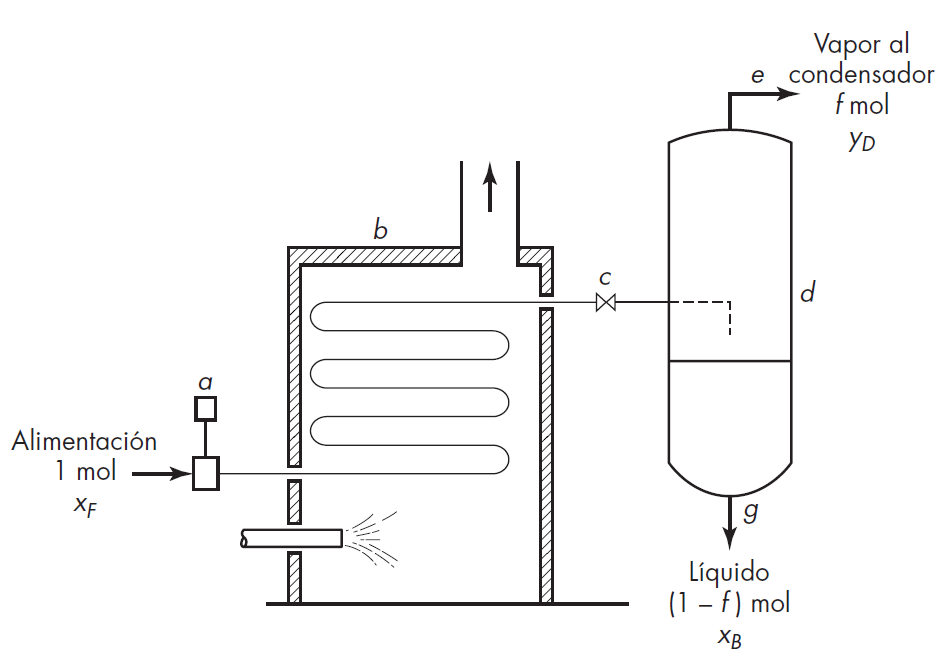
\includegraphics[width = 0.65\linewidth]{img/destilacion/DestilacionFlash_1.PNG}
    \caption{Planta de destilación flash o instantánea.}
    \label{fig:DestilacionFlash_1}
\end{figure}

La alimentación se hace circular por medio de la bomba $a$, a través del calentador $b$, y se reduce la presión en la válvula $c$. Una mezcla íntima de vapor y líquido entra en el separador $d$, en el que permanece el tiempo suficiente para permitir que se separen las corrientes de vapor y líquido. Debido al gran contacto existente entre el líquido y el vapor antes de su separación, las corrientes que se separan están en equilibrio. El vapor sale a través de la línea $e$ y el líquido a través de la línea $g$.

La destilación instantánea (destilación flash) se usa de manera extensa en la refinación del petróleo, en la cual sus fracciones se calientan en destiladores de tubos y el fluido calentado se evapora instantáneamente (flash) en corrientes de vapor y corrientes de líquido residuales, cada una de las cuales contiene muchos componentes.

\subsection{Destilación flash de mezclas binarias}

Supongamos que una mezcla de F moles de dos componentes (A y C) entra como alimentación al equipo presentado en la Figura \ref{fig:DestilacionFlash_1}. Adicioanlmente, definimos como $x_F$ la fracción molar del compuesto más volátil de la mezcla. Y llamamos al flujo molar de vapor en la zona superior $V$ y el flujo de cola de la zona inferior $B$, Tenemos que podemos plantear los siguientes balances:

Balance Global de Materia:
\begin{equation}
    \label{eq:Destilacion_0}
    F = V + B
\end{equation}

Balance de Materia del compuesto más volátil:
\begin{equation*}
    Fx_D = Vy_D + Bx_B
\end{equation*}

en donde $y_D$ y $x_B$ se definen como la fracción molar del compuesto más volátil en la zona superior e inferior, respectivamente. Si en la ecuación anterior definimos lo siguiente:

\begin{equation*}
    f = V/F
\end{equation*}

Entonces nuestra ecuación de Balance de Materia del compuesto más volátil nos queda de la siguiente manera:

\begin{equation}
    \label{eq:Destilacion_1}
    x_F = f y_D + (1-f) x_B
\end{equation}

En la ecuación \ref{eq:Destilacion_1} podemos apreciar que tenemos dos incognitas en el sistema $y_D$ y $x_B$. Entonces ahora debemos encontrar una forma que permita relacionar la concentración del compuesto volátil en el líquido y en el gas.

Para ello, si suponemos que el sistema en el equipo cuenta con el tiempo suficiente para alcanzar el equilibrio, tenemos que podemos aplicar las ecuaciones de equilibrio del Capítulo 1:

\begin{equation}
    \label{eq:Destilacion_2}
    \overline{f}_{iV} = \overline{f}_{iL}
\end{equation}

En forma rigurosa esta relación de equilibrio es la siguiente entre ambas fases es:

\begin{equation}
    \label{eq:Destilacion_3}
    K_i = \frac{\gamma_{iL} \phi_{iL}}{\overline{\phi}_{iV}}
\end{equation}

Si la solución que estamos destilando asumimos que se comporta como una solución ideal, es decir, $\gamma_{iL} = 1.0$, $\phi_{iL} = P_i^S$ y $\overline{\phi}_{iV} = 1.0$, tenemos que la ecuación \ref{eq:Destilacion_3} queda de la siguiente manera para el compuesto $i$:

\begin{equation}
    \label{eq:Destilacion_4}
    K_i = \frac{P_i^S}{P}
\end{equation}

donde $P$ es la presión del sistema y $P_i^S$ es la presión de vapor de $i$. Ahora si hacemos la relación entre los dos compuestos (el compuesto más volátil con el menos volátil), tenemos la siguiente relación llamada \textbf{volatilidad relativa}:

\begin{equation}
    \label{eq:Destilacion_5}
    \alpha_{AC} = \frac{y_{A,eq}/x_{A,eq}}{y_{C,eq}/x_{C,eq}} = \frac{K_A}{K_C}
\end{equation}

Y si asumimos una mezcla ideal, tenemos que la volatilidad relativa es igual a la razón entre presiones de vapor de los compuestos, es decir:

\begin{equation*}
    \alpha_{AC} = \frac{P_A^S}{P_C^S}
\end{equation*}

Con las diferentes formas de la formulación de la volatilidad relativa y considerando que en mezcla binarias se cumple lo siguiente:

\begin{equation*}
    x_C = 1 - x_A \hspace{0.75cm} \textrm{y} \hspace{0.75cm} y_C = 1-y_A
\end{equation*}

Tenemos que la ecuación \ref{eq:Destilacion_5} se puede reescribir de la siguiente forma:

\begin{equation}
    \label{eq:Destilacion_6}
    \alpha_{AC} = \frac{y_{A,eq}/x_{A,eq}}{(1-y_{A,eq})/(1-x_{A,eq})}
\end{equation}

y si reordenamos, podemos obtener una expresión útil para relacionar directamente la composición del vapor con la composición del liquido en un sistema binario:

\begin{equation}
    \label{eq:Destilacion_7}
    y_{A, eq} = \frac{\alpha_{AC} y_{A, eq}}{1 + (\alpha - 1)x_{A, eq}}
\end{equation}

Entonces utilizando las ecuaciones \ref{eq:Destilacion_1} y \ref{eq:Destilacion_7} es posible resolver el sistema de destilación flash que alcanza el equilibrio. Con respecto al parámetro $f$ generalmente no se fija directamente, sino que depende de la entalpía de la corriente que ingresa ($H_F$) y las entalpías de las corrientes que salen del sistema liquida ($H_x$) y vapor ($H_y$):

\begin{equation}
    \label{eq:Destilacion_8}
    H_F = f H_y + (1-f) H_x
\end{equation}

\section{Destilación Diferencial o Destilación Rayleigh}

Una modificación de la destilación flash consiste en la presentada en la Figura \ref{fig:DestiladorRayleigh} que fue utilizada por primera vez por Lord Rayleigh en 1902. En este tipo de destilación como se puede apreciar no existe el proceso de reflujo, es decir, no se devuelve una parte del proceso de destilado al sistema. En cualquier instante, se supone que el vapor que sale del destilador con la composición $y_D$ está en equilibrio con el líquido (residuo) de la bombona o alambique, que se supone que está perfectamente mezclado. En el condensador el vapor de pasa a líquido de manera completa (condensador total) y por tanto, $y_D$ = $xD$. Se supone que la bombona de destilación es la única etapa de equilibrio porque no hay bandejas encima de la bombona. Este aparato es útil para separar mezclas de punto de ebullición amplio.


\begin{figure}[H]
    \centering
    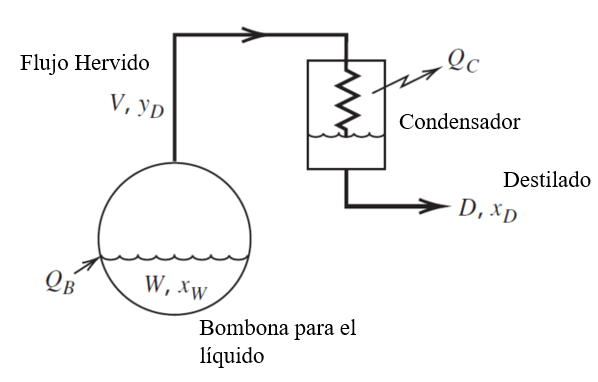
\includegraphics[width = 0.5\linewidth]{img/destilacion/Destilacion_Rayleigh.PNG}
    \caption{Destilador Rayleigh}
    \label{fig:DestiladorRayleigh}
\end{figure}

En la Figura \ref{fig:DestiladorRayleigh} podemos apreciar la siguiente nomenclatura:

\hspace{0.1cm}

\begin{tabular}{c c l}
     $D$ &=&  velocidad de destilado instantáneo, mol/h \\
    $Q_B$ &=&  tasa de entrada de calor a la bombona \\
    $Q_C$ &=&  tasa de salida de calor del condensador \\
    $V$ &=& tasa de vapor instantánea que va abandonando la bombona, mol/h \\ 
    $y$ &=& $y_D = x_D =$ fracción molar en destilado instantáneo dejando la olla inmóvil \\
    $W$ &=& moles de líquido (residuo) que quedan en la bombona \\
    $x$ &=& $x_W =$ fracción molar en el líquido (residuo)
\end{tabular}

Para cualquier componente de la mezcla, la tasa instantánea de salida $= D y_D$ es igual a la:

\begin{equation}
    \left. \begin{matrix}
        \textrm{Tasa instantánea de} \\
        \textrm{agotamiento en la bombona}
    \end{matrix} \right\}
     = - \frac{d}{dt} \left( W x_W \right) = -W \frac{dx_W}{dt} - x_W \frac{dW}{dt} 
\end{equation}

donde la tasa de destilado y, por lo tanto, la tasa de agotamiento de líquido en la bombona, dependen de la tasa de entrada de calor, $Q_B$, a la bombona. Reordenando la expresión anterior, el balance de un componente en cualquier instante es:

\begin{equation}
    \label{eq:Destilacion_9}
    \frac{d}{dt}(W x_W) = W \frac{dx_W}{dt} + x_W\frac{dW}{dt} = - Dy_D
\end{equation}

Y si multiplicamos la ecuación \ref{eq:Destilacion_9} por $dt$, obtenemos que:

\begin{equation*}
    W dx_W + x_WdW = y_D (- D dt) = y_D dW
\end{equation*}

ya que por balance total de material, $–Ddt = dW$. Separando variables e integrando de la condición de carga inicial de la bombona de $W_0$ (Moles de
Líquido en la bombona en el $t = 0$) y $x_{W_0}$ (Fraccion de moles líquido en la bombona en el $t = 0$),

\begin{equation}
    \label{eq:Destilacion_10}
    \int_{x_{W_0}}^{x_W} \frac{dx_W}{y_D-x_W} = \int_{W_0}^{W} \frac{dW}{W} = \ln \left( \frac{W}{W_0} \right)
\end{equation}
 
Esta es la ecuación de Rayleigh, que se aplicó por primera vez a la destilación por lotes de mezclas de punto de ebullición amplio como \ce{HCl-H2O}, \ce{H2SO4-H2O} y \ce{NH3-H2O}, donde una etapa es suficiente para lograr la separación deseada. Sin reflujo, se supone que $y_D$ y $x_W$ están en equilibrio, y la ecuación \ref{eq:Destilacion_10} se simplifica a:

\begin{equation}
    \label{eq:Destilacion_11}
    \int_{x_{W_0}}^{x} \frac{dx}{y-x} = \ln \left( \frac{W}{W_0} \right)
\end{equation}

La ecuación \ref{eq:Destilacion_11} se integra fácilmente cuando la presión es constante, el cambio de temperatura en la bombona destilada es relativamente pequeño (mezcla en punto de ebullición) y los valores K son independientes de la composición. Entonces $y = Kx$, donde si K es constante, La ecuación \ref{eq:Destilacion_11} se convierte en:

\begin{equation}
    \label{eq:Destilacion_12}
    \ln \left( \frac{W}{W_0} \right) = \frac{1}{K-1} \ln \left( \frac{x}{x_{W_0}} \right)
\end{equation}

Para una mezcla binaria, si la volatilidad relativa $\alpha$, en lugar de K, se asume constante, la ecuación \ref{eq:Destilacion_11} da:

\begin{equation}
    \label{eq:Destilacion_13}
    \ln \left( \frac{W_0}{W} \right) = \frac{1}{\alpha - 1} \left[ \ln \left( \frac{x_{W_0}}{x} \right) + \alpha \ln \left( \frac{1-x}{1-x_{W_0}} \right) \right]
\end{equation}

Si la relación de equilibrio $y = f(x)$ está como datos experimentales, la integración de la ecuación \ref{eq:Destilacion_11} se puede realizar gráfica o numéricamente.

\section{Columna de Destilación Contínua con Reflujo}

Los dos tipos de equipos de destilación anteriormente mencionados se utilizan esencialmente para la separación de componentes que tienen temperaturas de ebullición muy diferentes. Cuando se requiere separar compuestos con punto de ebullición (volatilidad) comparable, es necesaria la utilización de una columna de destilación contínua con reflujo tal como se muestra en la Figura \ref{fig:ColumnaDestilacion_1}

\begin{figure}[H]
    \centering
    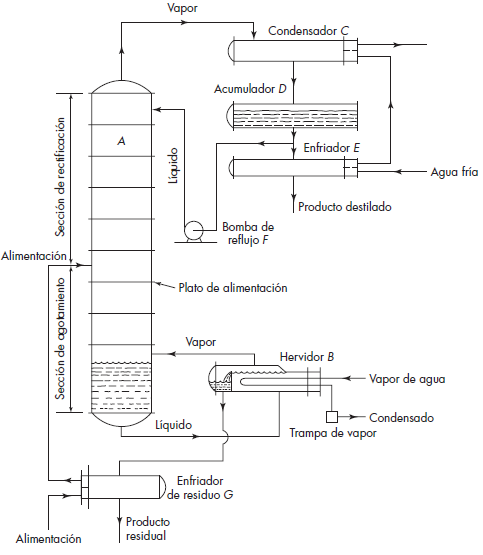
\includegraphics{img/destilacion/ColumnaDestilacion.PNG}
    \caption{Columna de Destilación continua con una sección de rectificación y agotamiento}
    \label{fig:ColumnaDestilacion_1}
\end{figure}

\subsection{Proceso de Fraccionamiento}

La torre de destilación contínua (Figura \ref{fig:ColumnaDestilacion_1}) consiste en una estructura cilíndrica divida en secciones por una serie de platos o bandejas (en ingles \textit{trays}) perforados que permite el flujo ascendentes de vapor y el flujo descendente de líquido. El vapor que se eleva por la columna, generalmente, pasa por un condensador y luego a través de un acumulador o un tambor de reflujo y un divisor de reflujo, parte del contenido se retira como el flujo Destilado (D), y el resto se devuelve a la columna com reflujo (R).

De manera paralela, en la zona inferior, el líquido que desciende, frecuentemente es calentado, ya sea a través de un flujo de vapor condensado o un flujo de aceite caliente, y el vapor que se genera por este calientamiento asciende por la torre pasando por estos platos perforados. En la Figura \ref{fig:ColumnaDestilacion_1} se muestra la disposición más comúnmente utilizada, que consta de un hervidor externo, donde el líquido del destilador pasa al hervidor y parte del flujo se evapora y se devuelve a la columna de destilación y otra parte sale como producto de cola de la columna (en ingles \textit{bottom}).

En esta columna, la alimentación se introduce en una zona intermedia de la columna y la zona superior a la alimentación se conoce como sección de rectificación o enriquemiento (\textit{rectifying section}) y la zona inferior a la alimentación se conoce como sección de agotamiento (\textit{stripping section}). La idea principal detrás de la teoría de una columan de destilación consiste en que el vapor que sale de un plato ideal estará en equilibrio con el líquido que sale, aunque en la práctica se producirá un menor grado de enriquecimiento.

En el analisis de la operación de un plato en una columna de destilación, es importante tener en cuenta que el vapor que ingresa al plato y el reflujo que fluye desde arriba hacia el plato no están en equilibrio y que las tasas adecuadas de transferencia de masa y calor son esenciales para el correcto funcionamiento del plato.

Estos platos presentes en una columna de destilación, presentan multiples perforaciones de aproximadamente 12 mm de diámetro y que si bien presentan diferentes configuraciones o modificaciones, el objetivo principal de estos platos es promover una buena mezcla de vapor y líquido con una baja caída de presión en el plato.

En cada plato, el sistema tiende a alcanzar al equilibrio porque:

\begin{itemize}
    \item Parte del componente menos volátil se condensa del vapor ascendente en el líquido aumentando así la concentración del componente más volátil (MVC) en el vapor.
    
    \item Parte del componente más volátil (MVC) se vaporiza desde el liquido en el plato, disminuyendo así la concentración del MVC en el líquido. 
\end{itemize}

\subsection{Acción de un plato ideal}

En un plato ideal de una columna de destilación, por definición, el líquido y el vapor que salen del plato se encuentran en equilibrio. Si consideramos un serie de platos ideales en donde suponenmos que se inician a enumerar los platos desde la zona superior de la columna (destilado) hasta la zona inferior (residuo o producto de cola) se obtiene el esquema presentado en la Figura \ref{fig:PlatoIdeal}. En donde los subíndices representan en todos los casos el punto de origen del flujo.

\begin{figure}
    \centering
    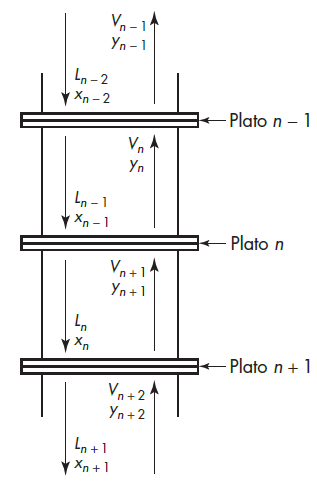
\includegraphics[width=0.4\linewidth]{img/destilacion/PlatoIdeal.PNG}
    \caption{Diagrama del balance de materia para el plato \textit{n}}
    \label{fig:PlatoIdeal}
\end{figure}

Si nos fijamos en la Figura \ref{fig:PlatoIdeal}, en el plato \textit{n} entran dos corrientes de fluido y salen otras dos. Una corriente de líquido $L_{n-1}$ mol/h, procedente del plato $n-1$ y una corriente de vapor $V_{n+1}$ mol/h, procedente del plato $n+1$, se ponen en contacto intimo debido a la presencia del plato ideal. Desde este plato ideal sale una corriente de vapor $V_n$ mol/h que asciende hacia el plato $n-1$, y una corriente de líquido $L_n$ mol/h, desciende hacia el plato $n+1$. Las corrientes de vapor se representa por la letra $V$ y las concentraciones de dichas corrientes se representan con la letra $y$ y las corrientes líquidas se representan con la letra $L$ y las concentraciones con la letra $x$.

Debido a la condición de plato ideal, tenemos que las concentraciones $x_n$ e $y_n$ están en equilibrio. Adicionalmente, por como opera la columna de destilación tenemos que a medida que ascendemos por los platos, tenemos que la concentración del compuesto más volátil va aumentando y a medida que descendemos por la columna la concentración del compuesto menos volátil también va en aumento. Este traspaso desde compuestos entre las fases ocurre debido a un proceso de vaporización y condensación de compuestos y ocurre debido a que ambas corrientes que ingresan al plato ideal están en su punto de burbuja (corriente líquida) y punto de rocío (corriente de vapor), permitiendo que la energía liberada por la condensación del compuesto menos volátil sirve para vaporizar el compuesto más volátil (En la Figura \ref{fig:DiagramaTemperaturaComposicion}) se muestra la ubicación espacial del plato ideal en un diagrama de Temperatura-Composición). Adicionalmente, como la concentración del compuesto volátil aumenta a medida que subimos por la columna de destilación, la temperatura de la corriente también disminuye (ya que se requiere menos temperatura para evaporar la corriente) y por tanto, la temperatura del plato $n$ resulta ser mayor que la del plato $n - 1$ y menor que la del plato $n + 1$.

\begin{figure}
    \centering
    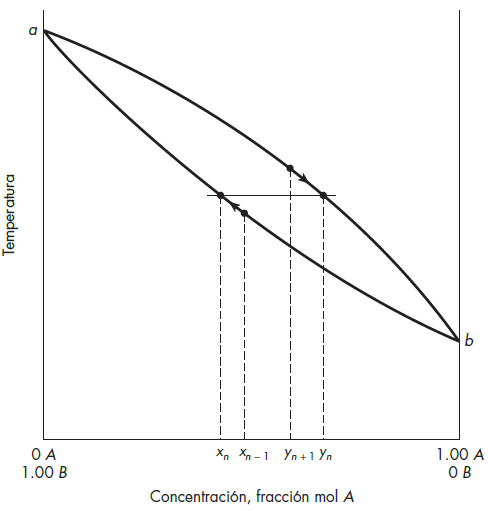
\includegraphics[width = 0.5\linewidth]{img/destilacion/DiagramaTemperaturaComposicion.PNG}
    \caption{Diagrama de la ubicación espacial de un plato ideal y los flujos de entrada}
    \label{fig:DiagramaTemperaturaComposicion}
\end{figure}

\subsection{Balance de materia en la columna de destilación fraccionada}

\subsubsection{Balances globales de materia para sistemas binarios}

La figura \ref{fig:ColumnaDestilacionPorParte} es un diagrama del balance de materia para una columna de destilación continua típica. La columna se alimenta con $F$ mol/h de concentración $x_F$ y genera $D$ mol/h del producto destilado de concentración $x_D$, y $B$ mol/h de producto residual de concentración $x_B$. 

\begin{figure}[H]
    \centering
    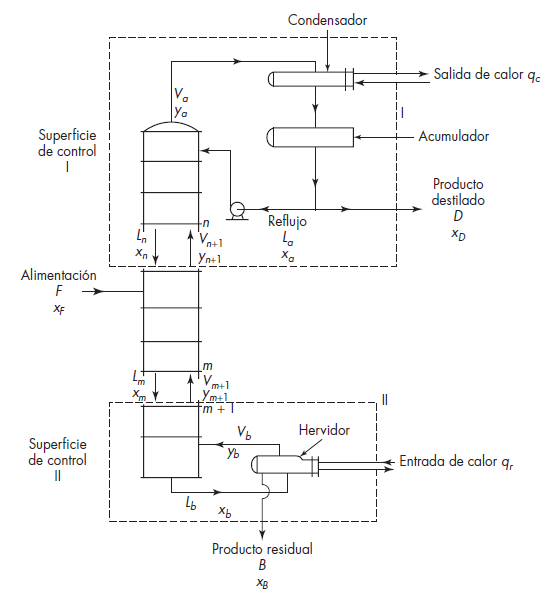
\includegraphics{img/destilacion/ColumnaDestilacionPorParte.PNG}
    \caption{Diagrama de balance de materia para una columna de fraccionamiento continuo.}
    \label{fig:ColumnaDestilacionPorParte}
\end{figure}

Con esta situación, es posible escribir dos balances globales de materia independientes:

\vspace{0.2cm}

\textbf{Balance total de materia}
\begin{equation}
    \label{eq:BalanceDestilacion_1}
    F = D + B
\end{equation}

\textbf{Balance del componente A}
\begin{equation}
    \label{eq:BalanceDestilacion_2}
    F x_F = D x_D + B x_B
\end{equation}

Sustituyendo $B$ de la ecuación \ref{eq:BalanceDestilacion_2} utilizando la ecuación \ref{eq:BalanceDestilacion_1}, se obtiene:

\begin{equation}
    \label{eq:BalanceDestilacion_3}
    \frac{D}{F} = \frac{x_F - x_B}{x_D - x_B}
\end{equation}

\subsubsection{Velocidades netas de flujo}

La magnitud $D$ es la diferencia entre las velocidades de flujo de las corrientes que entran y salen por la parte superior de la columna. Un balance de materia alrededor del condensador y del acumulador de la Figura \ref{fig:ColumnaDestilacionPorParte} conduce a:

\begin{equation}
    \label{eq:BalanceDestilacion_4}
    D = V_a - L_a
\end{equation}

Esta misma relación es aplicable a la zona encerrada en la zona superior de la Figura \ref{fig:ColumnaDestilacionPorParte}. Incluyendo a todos los platos por encima del plato $n+1$. Por lo tanto, el balance total de material en esa zona es:

\begin{equation}
    \label{eq:BalanceDestilacion_5}
    D = V_{n+1} - L_n
\end{equation}

Si nos fijamos, el flujo $D$ corresponden a la cantidad de materia que asciende por la columna y se denomina como \textit{velocidad neta de flujo}. 

De manera similar la balance total, si hacemos el balance para el compuesto A, obtenemos:

\begin{equation}
    \label{eq:BalanceDestilacion_6}
    D x_D = V_{a} y_a - L_a x_a = V_{n+1} y_{n+1} - L_n x_n
\end{equation}

De esta última ecuación, tenemos que el producto $Dx_D$ es la velocidad neta de flujo del componente A, que asciende en la sección superior de la columna y que es constante a través de esta parte del equipo.

En la zona inferior, se puede hacer de manera análoga el mismo análisis, obteniendo los siguientes balances:

\begin{equation}
    \label{eq:BalanceDestilacion_7}
    B = L_b - V_b = L_m - V_{m+1}
\end{equation}
\begin{equation}
    \label{eq:BalanceDestilacion_8}
    B x_B = L_b x_b - V_b y_b =  L_m x_m - V_{m+1} y_{m+1}
\end{equation}

Se utiliza el subíndice $m$ en lugar de $n$ para representar un plato general de la sección de agotamiento.

\subsubsection{Línea de Operación}

En una columna de destilación fraccionada, como hay dos secciones (secciones de rectificación y agotamiento), también existen dos líneas de operación: una para la sección de rectificación y otra para la sección de agotamiento. 

En la sección de rectificación o enriquecimiento, tenemos que el balance en un plato cualquiera, es el siguiente:

\textbf{Balance total en la zona de rectificación:}
\begin{align*}
    D = V_{n+1} - L_n \\
    (V_a-L_a) = V_{n+1} - L_n
\end{align*}
\begin{equation}
    \label{eq:BalanceDestilacion_9}
    L_a + V_{n+1} = L_n + V_a
\end{equation}

\textbf{Balance de materia del componente A en la zona de rectificación:}
\begin{equation}
    \label{eq:BalanceDestilacion_10}
    L_a x_a + V_{n+1} y_{n+1} = L_n x_n + V_a y_a
\end{equation}

De la ecuación \ref{eq:BalanceDestilacion_10} es posible hacer un reordenamiento de los términos, obteniendo la siguiente ecuación:

\begin{equation}
    \label{eq:BalanceDestilacion_11}
    y_{n+1} = \frac{L_n}{V_{n+1}} x_n + \frac{V_a y_a - L_a x_a}{V_{n+1}}
\end{equation}

Sin embargo, tenemos que el término $V_a y_a - L_a x_a$ es igual a $D x_D$, con ello, se obtiene lo siguiente:

\begin{equation}
    \label{eq:BalanceDestilacion_12}
    y_{n+1} = \frac{L_n}{V_{n+1}} x_n + \frac{D x_D}{V_{n+1}}
\end{equation}

De esta ecuación es posible deducir que la pendiente es la relación entre el flujo de la corriente de líquido y el de la corriente de vapor. Pero, de esta ecuación y por temas de conveniencia es posible sustituir el término de $V_{n+1}$ usando la ecuación \ref{eq:BalanceDestilacion_5}, obteniendo:

\begin{equation}
    \label{eq:BalanceDestilacion_13}
    y_{n+1} = \frac{L_n}{L_n + D} x_n + \frac{D x_D}{L_n + D}
\end{equation}

De manera análoga, en la sección de agotamiento el balance de materia del compuesto A es el siguiente:

\textbf{Balance Total de Materia en la zona de agotamiento:}
\begin{equation}
    \label{eq:BalanceDestilacion_14}
    V_{m+1} = L_{m} - B
\end{equation}

\textbf{Balance de Materia del componente A en la zona de agotamiento:}
\begin{equation}
    \label{eq:BalanceDestilacion_15}
    V_{m+1} y_{m+1} = L_{m} x_{m} - B x_{B}
\end{equation}

Reordenando la ecuación \ref{eq:BalanceDestilacion_15} es posible obtener lo siguiente:

\begin{equation}
    \label{eq:BalanceDestilacion_16}
    y_{m+1} = \frac{L_m}{V_{m+1}} x_m - \frac{B x_B}{V_{m+1}}
\end{equation}

La ecuación \ref{eq:BalanceDestilacion_16} es conocida como la \textit{línea de operación en la sección de agotamiento}. De nuevo, la pendiente es la relación entre el flujo de líquido y el flujo de vapor. Sustituyendo el término $V_{m+1}$ utilizando la ecuación \ref{eq:BalanceDestilacion_7}, se obtiene lo siguiente:

\begin{equation}
    \label{eq:BalanceDestilacion_17}
    y_{m+1} = \frac{L_m}{L_m - B} x_m - \frac{B x_B}{L_m - B}
\end{equation}

La ecuación \ref{eq:BalanceDestilacion_13} muestra que la pendiente de la línea de operación en la sección de rectificación siempre es menor que 1.0; en la sección de agotamiento, la pendiente siempre es mayor que 1.0, como se indica en la ecuación \ref{eq:BalanceDestilacion_17}.


\subsection{Método de McCabe-Thiele}

Uno de los métodos más utilizados dentro de la industria es la metodología de determinación del número de platos \textit{ideales} para una mezcla binaria y este método se llama \textit{Método McCabe-Thiele}. Para este método se utilizan las ecuaciones de las líneas de operacion de ambas secciones (ecuaciones \ref{eq:BalanceDestilacion_13} y \ref{eq:BalanceDestilacion_17}) y la curva de equilibrio en el diagrama xy. Sin embargo, en las ecuaciones \ref{eq:BalanceDestilacion_13} y \ref{eq:BalanceDestilacion_17} se observa que, a menos que $L_n$ y $L_m$ sean constantes, las líneas de operación son curvas y sólo es posible representarlas de forma gráfica si se conoce la variación de estás corrientes internas con concentración. En el caso general se necesitan balances de entalpía para determinar la posición de una línea de operación curva, pero este tema lo trataremos más adelante en este capítulo.

\subsubsection{Sobreflujo molar constante}

Uno de los fenómenos que ocurre normalmente en las columnas de destilación fraccionada, es que lo flujos molares de vapor y de líquido son casí constantes en toda la columna y por consiguiente las líneas de operación son casí líneas rectas.


Este fenómeno proviene del hecho de que a medida que el vapor asciende por la columna, 1 mol que se condensa suminstra energía para vaporizar alrededor de 1 mol que desciende, esto conduce a decir que las \textbf{entalpías de evaporación son casí iguales}.

Con estos antedecentes, uno de los supuestos que se hace en la industría cuando se realiza el diseño de una columan de destilación, es considerar que existe \textit{sobreflujo molar constante}. Este concepto consiste en en asumir que los flujos molares en la zona superior de la columna son constante y por tanto los subíndices $n$ y $n+1$ se pueden suprimir quedando solamente $L$ y $V$. Y lo mismo se puede aplicar a la zona inferior de la columna, suprimiendo los términos $m$ y $m+1$ quedando los términos $\overline{L}$ y $\overline{L}$ para hacer referencia a los flujos molares de líquido y vapor en la zona inferior de la columan. 

En este modelo simplificado, las ecuaciones de balance de materia son lineales
y las líneas de operación, rectas y una línea de operación se puede graficar si se conocen las coordenadas de dos puntos sobre ella.


\subsubsection{Relación de Reflujo}

Otro concepto útil que normalmente se utiliza en el diseño de una columna de destilación, es la \textit{relación de reflujo}. Una de sus formas es la relación entre el flujo que se devuelve a la torre desde la sección de rectificación (\textit{reflujo}) y el producto destilado, con esta definición la relación es la siguiente:

\begin{equation}
    \label{eq:BalanceDestilacion_18}
    R_D = \frac{L}{D} = \frac{V-D}{D}
\end{equation}

Con esta definición, la ecuación \ref{eq:BalanceDestilacion_13} se puede multiplir por D/D a ambos lados de la ecuación para obtener lo siguiente:

\begin{equation*}
    y_{n+1} = \frac{L/D}{(L+D)/D}x_n + \frac{(D/D) x_D}{(L+D)/D}
\end{equation*}
\begin{equation}
    \label{eq:BalanceDestilacion_19}
    y_{n+1} = \frac{R_D}{R_D + 1}x_n + \frac{x_D}{R_D + 1}
\end{equation}

Tal como habíamos mencioando anteriormente, la ecuación \ref{eq:BalanceDestilacion_19} es la línea de operación de la sección de rectificación en términos del reflujo. Su pendiente es $R_D/(R_D+1)$. La intercepción con el eje $y$ es cuando la concentración de vapor es igual a $x_D/(R_D + 1)$.

En general, el valor $x_D$ está fijado por las condiciones de diseño, mientras que la relación de reflujo $R_D$ es una variable de operación que se puede controlar a voluntad ajustando la porción entre el reflujo y el producto destilado, o bien modificando la cantidad de vapor que se forma en el hervidor para una velocidad de flujo dada del producto destilado. 

Otro punto que se puede obtener de la línea de opéración de la ecuación \ref{eq:BalanceDestilacion_19} es cuando $x_n$ toma el vapor del destilado $x_D$, con ello:

\begin{equation}
    \label{eq:BalanceDestilacion_20}
    y_{n+1} = \frac{R_D}{R_D + 1} x_D + \frac{x_D}{R_D +1} = \frac{x_D (R_D+1)}{R_D + 1} = x_D
\end{equation}

La línea de operación para la sección de rectificación intercepta la diagonal en el punto $(x_D, x_D)$. Esto se cumple tanto para un condensador total como para uno parcial. 

\subsubsection{Condensado y Plato Superior}

Uno de los temas a decidir al momento de diseñar una columna de destilación, es determinar el tipo de condensador en la zona superior de la columna. En la Figura \ref{Fig:PlatoSuperior_A} es posible apreciar el balance general de flujos que ocurre en la zona superior de la columna. 

Para la generación del flujo líquido $L_C$ es posible hacerlo usando un condensador total (Figura \ref{Fig:PlatoSuperior_B}) o usando un condensador parcial (Figura \ref{Fig:PlatoSuperior_C}). 

En el caso de la Figura \ref{Fig:PlatoSuperior_A}, en donde se utiliza un condensador total, las concentraciones del vapor que procede del plato superior, la del reflujo que va a dicho plato y la del producto destilador son iguales y todas pueden representarse por $x_D$. El extremo de la línea de operación es el punto $(x_D, x_D)$, que es la intersección de la línea de operación con la diagonal. El triángulo abc de la Figura \ref{Fig:PlatoSuperiorDiagrama_A} representa el plato superior en la columna.

Cuando se utiliza un condensador parcial, el líquido de reflujo no tiene la misma composición que el producto destilado; es decir, $x_C \equiv x_D$, y se genera una configuración parecida a la presentada en la Figura \ref{Fig:PlatoSuperior_C}. El vapor que sale del condensador parcial tiene una composición $y'$, que es la misma que $x_D$. En estas condiciones es aplicable el diagrama de la Figura \ref{Fig:PlatoSuperiorDiagrama_B}. La línea de operación pasa por el punto $(x_D, x_D)$ de la diagonal, pero, por lo que a la columna se refiere, la línea de operación termina en el punto $a'$, que tiene de coordenadas $(x_C, y_1)$. El triángulo $a'b'c'$ de la Figura \ref{Fig:PlatoSuperiorDiagrama_B} representa el plato superior de la columna. Puesto que el vapor que sale de un condensador parcial está normalmente en equilibrio con el líquido condensado, la composición del vapor $y'$ es el valor de la ordenada de la curva de equilibrio donde la abscisa es $x_C$, tal como se indica en la Figura \ref{Fig:PlatoSuperiorDiagrama_B}. El condensador parcial, representado por el triángulo de trazos discontinuos $aba'$ de la Figura \ref{Fig:PlatoSuperiorDiagrama_B}, es por lo tanto equivalente a una etapa teórica adicional del aparato de destilación.


\begin{figure}
  \begin{subfigure}[b]{0.28\textwidth}
    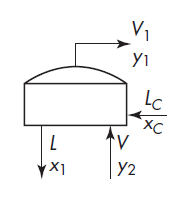
\includegraphics[width=\textwidth]{img/destilacion/PlatoSuperior_A.PNG}
    \caption{ }
    \label{Fig:PlatoSuperior_A}
  \end{subfigure}
  \hfill
  \begin{subfigure}[b]{0.3\textwidth}
    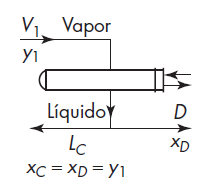
\includegraphics[width=\textwidth]{img/destilacion/PlatoSuperior_B.PNG}
    \caption{ }
    \label{Fig:PlatoSuperior_B}
  \end{subfigure}
  \begin{subfigure}[b]{0.3\textwidth}
    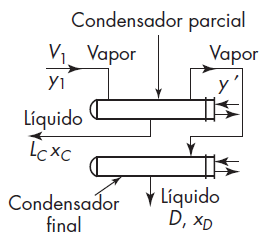
\includegraphics[width=\textwidth]{img/destilacion/PlatoSuperior_C.PNG}
    \caption{ }
    \label{Fig:PlatoSuperior_C}
  \end{subfigure}
  \caption{Diagramas de los balances de materia para el plato superior y el condensador: a) plato superior; b) condensador total; c) condensadores parcial y final.}
  \label{Fig:PlatoSuperior}
\end{figure}

\begin{figure}
  \begin{subfigure}[b]{0.45\textwidth}
    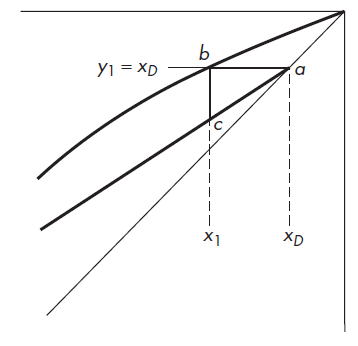
\includegraphics[width=\textwidth]{img/destilacion/PlatoSuperiorDiagrama_A.PNG}
    \caption{ }
    \label{Fig:PlatoSuperiorDiagrama_A}
  \end{subfigure}
  \hfill
  \begin{subfigure}[b]{0.45\textwidth}
    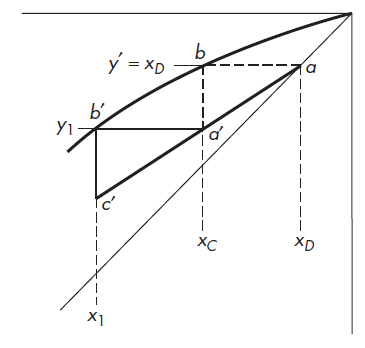
\includegraphics[width=\textwidth]{img/destilacion/PlatoSuperiorDiagrama_B.PNG}
    \caption{ }
    \label{Fig:PlatoSuperiorDiagrama_B}
  \end{subfigure}
  \caption{Construcción gráfica para el plato superior: a) utilizando un
condensador total; b) utilizando condensadores parcial y final.}
   \label{Fig:PlatoSuperiorDiagrama}
\end{figure}

\subsubsection{Plato en el fondo de la columna y hervidor}

De manera análoga a lo mencionado en la zona superior de la columna, en la zona inferior, la ecuación \ref{eq:BalanceDestilacion_17} asumiendo flujos molares constantes en la zona de agotamiento, sustituyendo los términos $L_m$ y $V_m$ por $\overline{L}$ y $\overline{V}$, obteniendo la siguiente ecuación:

\begin{equation}
    \label{eq:BalanceDestilacion_21}
    y_{m+1} = \frac{\overline{L}}{\overline{L} - B} x_m - \frac{B x_B}{\overline{L} - B}
\end{equation}

Esta ecuación es también conocida como \textit{línea de operación de la sección de agotamiento}, en donde se cumple que si $x_m$ es igual a $x_B$, entonces obtenemos que $y_{m+1}$ es igual a $x_B$.

A la salida de la sección de agotamiento, generalmente, el caudal de líquido se conecta a un hervidor o \textit{boiler} parcial con tal de evaporar una fracción del líquido y poder devolver ese vapor a la columna. Este esquema es el que está representado en la Figura \ref{fig:DestiladorHervidor}

\begin{figure}[H]
    \centering
    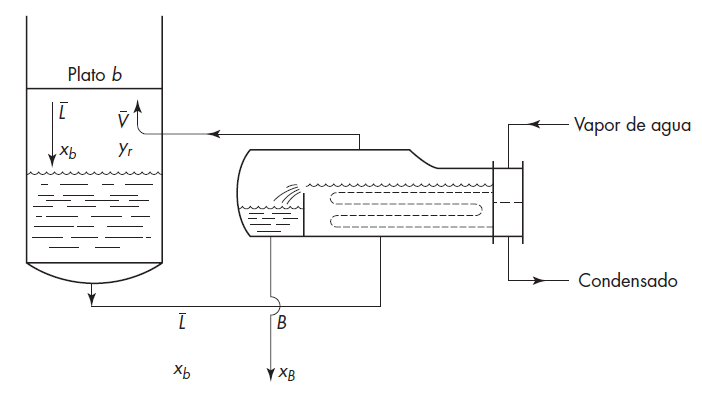
\includegraphics{img/destilacion/DestiladorHervidor.PNG}
    \caption{Diagrama de los balances de materia para el plato inferior y el intercambiador de calor.}
    \label{fig:DestiladorHervidor}
\end{figure}

\subsubsection{Plato de Alimentación}

En una sección intermedia de la columan existe un plato al cual, adicional a los flujos que van entrando de los otros platos de la columna, existe un plato que recibe el flujo de alimentación de la columna, por eso ese plato se conoce como \textit{Plato de Alimentación}. 

Esta mezcla que alimenta a la columna puede tomar diferentes esquemas que están representados en la Figura \ref{fig:PlatoAlimentacionDestilacion} en función a la condición del flujo de alimentación. 

En la figura Figura \ref{fig:PlatoAlimentacionDestilacion}a se supone que la alimentación está fría y que toda la corriente de alimentación se suma al líquido que desciende por la columna. Además algo de vapor se condensa para calentar la alimentación hasta el punto de burbuja; esto da lugar a que el flujo de líquido sea aun mayor en la sección de agotamiento y a que disminuya el flujo de vapor en la sección de rectificación.

En la Figura \ref{fig:PlatoAlimentacionDestilacion}b se supone que la alimentación está en su punto de burbuja. No se requiere condensación para calentar la alimentación, de forma que $V = \overline{V}$ y $\overline{L} = F+L$.

Si la alimentación está parcialmente en forma de vapor, como indica la Figura \ref{fig:PlatoAlimentacionDestilacion}c, la porción de líquido de la alimentación forma parte de $\overline{L}$ y la porción de vapor forma parte de $V$.

Si la alimentación es vapor saturado, como muestra la Figura \ref{fig:PlatoAlimentacionDestilacion}d, toda la alimentación forma parte de $V$, de modo que $L = \overline{L}$ y $V = F + \overline{V}$.

Finalmente, si la alimentación es vapor sobrecalentado, como en la Figura \ref{fig:PlatoAlimentacionDestilacion}e, parte del líquido procedente de la sección de rectificación se vaporiza con el fin de enfriar la alimentación hasta el estado de vapor saturado. 

\begin{figure}[H]
    \centering
    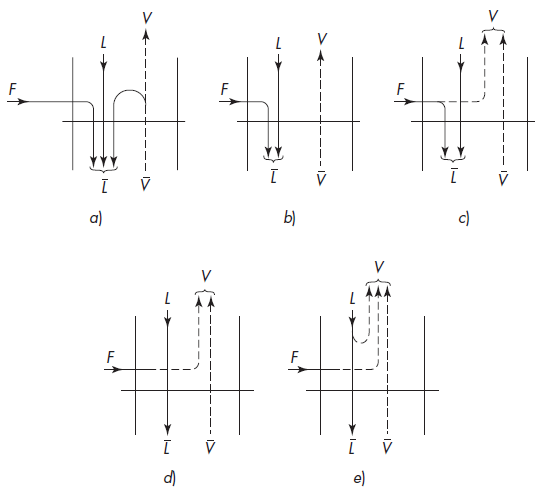
\includegraphics{img/destilacion/PlatoAlimentacion.png}
    \caption{Flujo a través del plato de alimentación para diferentes condiciones de alimentación: a) alimentación como líquido frío; b) alimentación como líquido saturado; c) alimentación parcialmente vaporizada; d) alimentación como vapor saturado; e) alimentación como vapor sobrecalentado}
    \label{fig:PlatoAlimentacionDestilacion}
\end{figure}


Es posible caracterizar los cinco tipos de alimentación utilizando un único factor, representado por $q$ y definido como los moles de líquido que fluyen en la sección de agotamiento como consecuencia de la introducción de cada mol de alimentación. Por tanto, $q$ tiene los siguientes límites numéricos para las distintas condiciones:

\begin{itemize}
    \item Alimentación fría, $q > 1$
    \item Alimentación en el punto de burbuja (líquido saturado), $q = 1$
    \item Alimentación parcialmente como vapor, $0 < q < 1$
    \item Alimentación en el punto de rocío (vapor saturado), $q = 0$
    \item Alimentación como vapor sobrecalentado, $q < 0$
\end{itemize}

Si la alimentación es una mezcla de líquido y vapor, $q$ es la fracción de líquido. Tal alimentación puede producirse por una evaporación instantánea (o flash) de equilibrio, de forma que $q = 1 – f$, donde $f$ es la fracción de la corriente original vaporizada en el flash.

El valor de $q$ para la alimentación como líquido frío se obtiene a partir de la ecuación

\begin{equation}
    \label{eq:BalanceDestilacion_22}
    q = 1 + \frac{c_{p,L} (T_b -T_F)}{\lambda}
\end{equation}

Para vapor sobrecalentado la ecuación es

\begin{equation}
    \label{eq:BalanceDestilacion_23}
    q = - \frac{c_{p,V} (T_F -T_d)}{\lambda}
\end{equation}

donde

\hspace{0.25cm}

\begin{tabular}{r c p{12.5cm}}
    $c_{p,L}$, $c_{p,V}$ & = & calores específicos del líquido y el vapor, respectivamente \\
    $T_F$ & = & temperatura de la alimentación \\
    $T_b$, $T_d$ & = & temperaturas del punto de burbuja y del punto de rocío de la alimentación, respectivamente \\
    $\lambda$ & = & calor de vaporización
\end{tabular}

\subsubsection{Línea de alimentación}

El valor de q obtenido a partir de la ecuación \ref{eq:BalanceDestilacion_22} o \ref{eq:BalanceDestilacion_23} se utiliza con los balances de materia para encontrar el lugar de todos los puntos de intersección de las líneas de operación. La ecuación para esta línea de intersecciones se obtiene como se indica a continuación.

La contribución de la corriente de alimentación al flujo interno de líquido es $qF$, de forma que la velocidad de flujo total del reflujo en la sección de agotamiento es

\begin{equation}
    \label{eq:BalanceDestilacion_24}
    \overline{L} = L + qF \hspace{0.75cm} \textrm{y} \hspace{0.75cm} \overline{L}-L = qF
\end{equation}

De manera análoga, la contribución de la corriente de alimentación al flujo interno de vapor es $F(1 – q)$, y por tanto la velocidad de flujo total de vapor en la sección de rectificación es

\begin{equation}
    \label{eq:BalanceDestilacion_25}
    V = \overline{V} + (1-q)F \hspace{0.75cm} \textrm{y} \hspace{0.75cm} V - \overline{V} = (1-q)F
\end{equation}

Para sobreflujo molar constante, las ecuaciones de los balances de materia para las dos secciones son

\begin{equation}
    \label{eq:BalanceDestilacion_26}
    V y_n = L x_{n+1} + D x_D
\end{equation}
\begin{equation}
    \label{eq:BalanceDestilacion_27}
    \overline{V} y_m = \overline{L} x_{m+1} - B x_B
\end{equation}

Para localizar el punto de intersección de las líneas de operación, sea $y_n = y_m$ y $x_{n+1} = x_{m+1}$, y al restar la ecuación \ref{eq:BalanceDestilacion_27} de la ecuación \ref{eq:BalanceDestilacion_26}:

\begin{equation}
    \label{eq:BalanceDestilacion_28}
    y \left( V - \overline{V} \right) = \left( L - \overline{L} \right) x + Dx_D + B x_B
\end{equation}

A partir de la ecuación \ref{eq:BalanceDestilacion_2}, los dos últimos términos de la ecuación \ref{eq:BalanceDestilacion_28} se sustituyen por $Fx_F$. Por otra parte, al sustituir $L - \overline{L}$ de la ecuación \ref{eq:BalanceDestilacion_24} y $V - \overline{V}$ de la ecuación \ref{eq:BalanceDestilacion_25} y simplificando se llega a

\begin{equation}
    \label{eq:BalanceDestilacion_29}
   y = - \frac{q}{1-q} x + \frac{x_F}{1-q}
\end{equation}

La ecuación \ref{eq:BalanceDestilacion_29} representa una línea recta, que recibe el nombre de \textit{línea de alimentación}, sobre la que están situadas las intersecciones de las líneas de operación. La posición de la líneas depende sólo de $x_F$ y de $q$. La pendiente de la línea de alimentación es $-q/(1 – q)$ y, como es posible demostrar sustituyendo $x$ por $y$ en la ecuación \ref{eq:BalanceDestilacion_29} y simplificando, la línea corta a la diagonal en $x = x_F$.

\subsubsection{Construcción de líneas de operación}

El método más senciloo para representar las líneas de operación consiste en los siguiente pasos:

\begin{enumerate}
    \item Localizar la línea de alimentación
    \item Calcular el eje $y$ que intercepta a $x_D/(R_D+1)$ de la línea de rectificación y representar en forma gráfica la línea que pasa por la intersección y el punto ($x_D$, $x_D$).
    \item Trazar la línea de agotamiento que pasa por el punto ($x_B$, $x_B$) y la intersección de la línea de rectificación con la línea de alimentación.
\end{enumerate}

Este procedimiento descrito se presenta en la Figura \ref{fig:LineasOperacion}.

\begin{figure}[H]
    \centering
    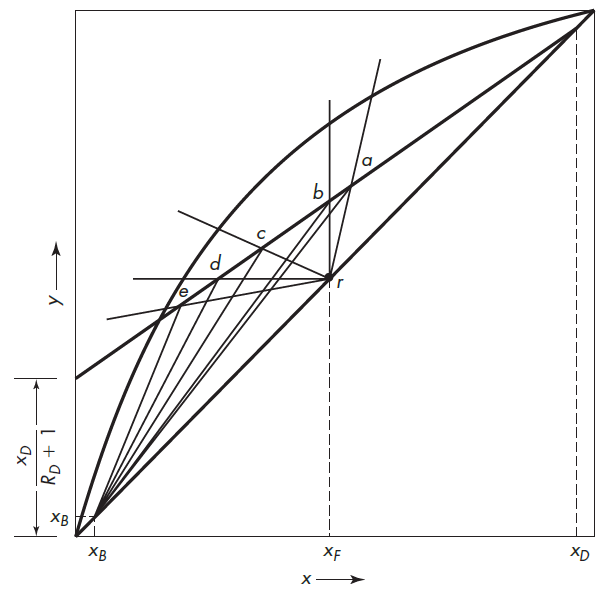
\includegraphics[width = 10cm]{img/destilacion/OperationLines.PNG}
    \caption{Efecto de la condición de la alimentación sobre la línea de alimentación: $ra$, alimentación como líquido frío; $rb$, alimentación como líquido saturado; $rc$, alimentación parcialmente vaporizada; $rd$, alimentación como vapor saturado; $re$, alimentación como vapor sobrecalentado.}
    \label{fig:LineasOperacion}
\end{figure}


\subsubsection{Localización del Plato de Alimentación}

Una vez representadas en forma gráfica las líneas de operación, el número de platos ideales se obtiene empleando la construcción habitual de paso por paso (escalones), tal como se ilustra en la Figura \ref{Fig:LineaOperacion_Ejemplo}.

La construcción puede comenzarse indistintamente por la parte inferior de la línea de agotamiento o por la parte superior de la línea de rectificación. En lo sucesivo se supone que la construcción comienza por la parte superior y que, además, se utiliza un condensador total. Al acercarse a la intersección de las líneas de operación, hay que decidir cuándo los escalones deben trasladarse de la línea de rectificación a la línea de agotamiento. El cambio deberá realizarse de tal forma que se obtenga el máximo enriquecimiento por plato con el fin de que el número total de platos de la columna sea mínimo.

El plato de alimentación siempre está representado por el triángulo que tiene un vértice en la línea de rectificación y otro en la de agotamiento. 

El traslado de una línea de operación a otra, y por lo tanto la localización del plato de alimentación, puede hacerse en cualquier lugar entre los puntos $a$ y $b$ de la Figura \ref{Fig:LineaOperacion_Ejemplo}; pero si el plato de alimentación está localizado en cualquier otro punto distinto del óptimo se precisa un número de plato innecesariamente más grande. Por ejemplo, si en la Figura \ref{Fig:LineaOperacion_B} el plato de alimentación es el número 7, los pasos más pequeños representados por la línea de trazos discontinuos da lugar a un requerimiento de 8 platos ideales más el hervidor, mientras que si la alimentación se introduce en el plato número 5 basta con 7 platos y el hervidor (Figura \ref{Fig:LineaOperacion_A}).

\begin{figure}[H] 
  \begin{subfigure}[b]{0.45\textwidth}
    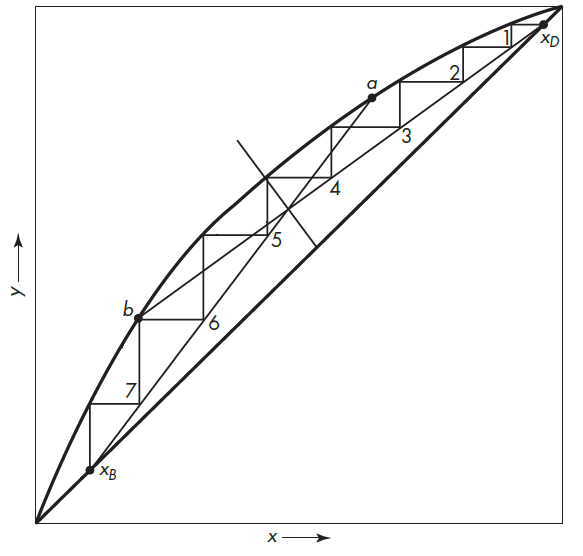
\includegraphics[width=\textwidth]{img/destilacion/Lineas_Operacion_A.png}
    \caption{ }
    \label{Fig:LineaOperacion_A}
  \end{subfigure}
  \hfill
  \begin{subfigure}[b]{0.45\textwidth}
    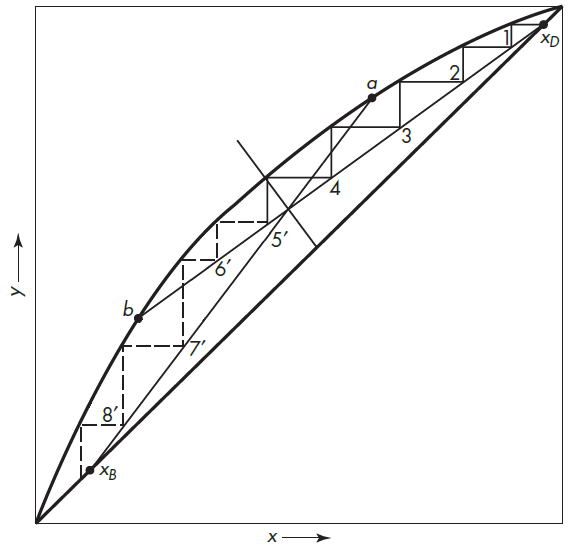
\includegraphics[width=\textwidth]{img/destilacion/Lineas_Operacion_B.png}
    \caption{ }
    \label{Fig:LineaOperacion_B}
  \end{subfigure}
  \caption{Localización del plato óptimo de alimentación: (a) \rule[.5ex]{2em}{.4pt} con alimentación en el plato 5 (localización
óptima), (b) \rule[.5ex]{0.5em}{.4pt} \rule[.5ex]{0.5em}{.4pt} \rule[.5ex]{0.5em}{.4pt} con alimentación en el plato 7.}
   \label{Fig:LineaOperacion_Ejemplo}
\end{figure}

\subsubsection{Número Mínimo de Platos}

Puesto que la pendiente de la línea de operación de la zona de rectificación es igual a $R_D/(R_D+1)$. De este término es posible notar que tiende a uno, cuando el valor de $R_D$ tiende a infinito. Cuando esta situación ocurre la línea de operación coincide entonces con la diagonal de la gráfica x vs y. Esta situación se conoce como \textit{Reflujo Total}.

Cuando el reflujo es total, se tiene que el número de plato de destilación es mínimo. Esta situación plantea la situación limitante de la columna de destilación. En esta situación, no no hay alimentación en la columna cuando opera el reflujo total, no existe discontinuidad entre las secciones superior e inferior.

En el caso de mezclas ideales, existe un método sencillo para la determinación del número de platos mínimos ($N_{\textrm{min}}$), y consiste en utilizar el término de volatilidad relativa de los compuestos a destilar y que se define de acuerdo a las concentraciones de los compuestos en equilibrio:

\begin{equation}
    \label{volatilidad_platosminimos}
    \alpha_{A,B} = \frac{\sfrac{y_{A,e}}{x_{A,e}}}{\sfrac{y_{B,e}}{x_{B,e}}}
\end{equation}

Una forma útil de la ecuación \ref{volatilidad_platosminimos} para encontrar $y_e$ en función de $x_e$ es:

\begin{equation}
    y_e = \frac{\alpha_{A,B} \cdot x_e}{1+(\alpha_{A,B}-1)\cdot x_e}
\end{equation}

En una mezcla ideal que sigue la ley de Raoult, y que la volatilidad relativa es la relacion entre las presiones de vapor, por lo que tendríamos lo siguiente:

\begin{align*}
    p_A &= P_A'\cdot x_A & y_A = \frac{p_A}{P}
\end{align*}
\begin{align*}
    p_B &= P_B'\cdot x_B & y_B = \frac{p_B}{P}
\end{align*}
\begin{equation}
    \alpha_{A,B} = \frac{\sfrac{y_{A,e}}{x_{A,e}}}{\sfrac{y_{B,e}}{x_{B,e}}} = \frac{\sfrac{P_A'}{P}}{\sfrac{P_B'}{P}} = \frac{P_A'}{P_B'}
\end{equation}

Para un sistema binario, $y_A/y_B$ y $x_A/x_B$ se sustituye por $y_A/(1-y_A)$ y $x_A/(1-x_A)$, de forma que para el plato $N+1$ la ecuación \ref{volatilidad_platosminimos} se escribe de la siguiente manera:

\begin{equation}
    \label{volatividad_plato_siguiente}
    \frac{y_{n+1}}{(1-y_{n+1})} = \alpha_{A,B} \cdot \frac{x_{n+1}}{(1-x_{n+1})}
\end{equation}

Cuando existe un reflujo total, tenemos de $D = 0$ y $L/V = 1$, $y_{n+1} = x_{n}$. Por lo que la ecuación \ref{volatividad_plato_siguiente} se puede escribir de la siguiente manera:

\begin{equation}
    \frac{x_{n}}{(1-x_{n})} = \alpha_{A,B} \cdot \frac{x_{n+1}}{(1-x_{n+1})}
\end{equation}.

Y si se utiliza un condensador total, tenemos que $y_1 = x_D$, por lo que la ecuación se transforma a lo siguiente:

\begin{equation}
    \label{ecuacionplatosminimos}
    \frac{x_{D}}{(1-x_{D})} = \alpha_{A,B} \cdot \frac{x_{1}}{(1-x_{1})}    
\end{equation}

y si escribimos las ecuaciones para los n platos del destilador:

\begin{align*}
    \frac{x_{1}}{(1-x_{1})} = \alpha_{A,B} \cdot \frac{x_{2}}{(1-x_{2})} \\
    ............................................ \\
    \frac{x_{n-1}}{(1-x_{n-1})} = \alpha_{A,B} \cdot \frac{x_{n}}{(1-x_{n})} \\
\end{align*}

Si la ecuación \ref{ecuacionplatosminimos} y todas las ecuaciones del conjunto de las ecuaciones de los n platos se multiplican entre sí al tiempo que se eliminan los términos intermedios, entonces:

\begin{equation}
    \label{ecuacionplatosminimos2}
    \frac{x_{D}}{(1-x_{D})} = (\alpha_{A,B})^{n} \cdot \frac{x_{n}}{(1-x_{n})}
\end{equation}

Para alcanzar la composición de descarga del fondo de la columna hacen falta $N_{\textrm{min}}$ platos y un intercambiador de calor, y la ecuación \ref{ecuacionplatosminimos2} se transforma en:

\begin{equation}
    \label{ecuacionplatosminimos3}
    \frac{x_{D}}{(1-x_{D})} = (\alpha_{A,B})^{N_{\textrm{min}}+1} \cdot \frac{x_{B}}{(1-x_{B})}
\end{equation}

Resolviendo por logaritmos la ecuación para $N_{\textrm{min}}$ se obtiene:

\begin{equation}
     \label{ecuacionplatosminimos4}
     N_{\textrm{min}} = \frac{\ln{\left[\frac{x_D \cdot (1-x_B)}{x_B \cdot (1-x_D)}\right]}}{\ln{\alpha_{A,B}}}-1
\end{equation}

La ecuación \ref{ecuacionplatosminimos4} es la \textit{ecuación de Fenske}, la cual se aplica cuando $\alpha_{A,B}$ es constante. Si la variación del valor de $\alpha_{A,B}$ desde el fondo de la columna hasta la parte superior es moderada, se recomienda para $\alpha_{A,B}$la media geométrica de los valores extremos.


\subsubsection{Relación de Reflujo Mínimo}

Para un reflujo inferior al total, el número de platos que se requieren para una separación dada es mayor que para el reflujo total, y aumenta de forma continua a medida que disminuye la relación de reflujo. A medida que la relación disminuye, el número de platos se hace muy grande y, para un valor mínimo definido, llamado \textit{relación de reflujo mínima}, el número de platos se hace infinito. 

Todas las columnas reales que producen una cantidad finita de los productos deseados de destilado y de residuo han de operar con una relación de reflujo comprendida entre el valor mínimo, para el que el número de platos es infinito, y una relación de reflejo infinito, para cuando el número de platos es mínimo.

Si $L_a/D$ es la relación de reflujo de operación y $(L_a/D)_{\textrm{min}}$ es la relación de reflujo mínima, entonces

\begin{equation}
    \label{eq:EcuacionReflujoMinimoDestilacion}
    \left( \frac{L_a}{D} \right)_{\textrm{min}} < \frac{L_a}{D} < \infty
\end{equation}

\begin{figure}[H]
    \centering
    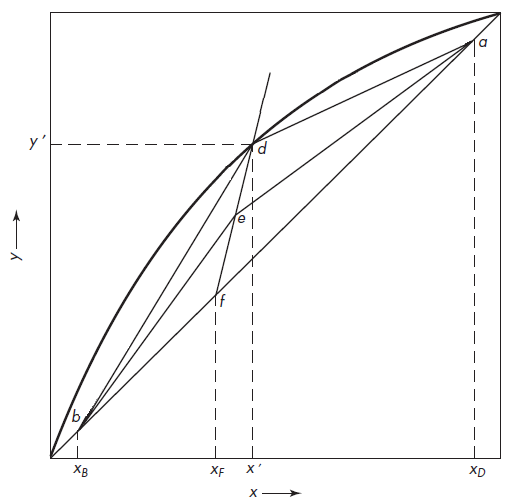
\includegraphics{img/destilacion/ReflujoMinimoDestilacion.png}
    \caption{Relacion de Reflujo Mínimo}
    \label{fig:ReflujoMinimo_Destilacion}
\end{figure}

En la Figura \ref{fig:ReflujoMinimo_Destilacion} se puede apreciar que las líneas $ae$ y $be$ corresponden a las líneas de operaciones de rectificación y agotamiento, respectivamente, que uno ve típicamente en una columna de destilación. Sin embargo, a medida que se va reduciendo el reflujo,
la intersección de las líneas de operación se va desplazando a lo largo de la línea de alimentación hacia la curva de equilibrio, el área del diagrama disponible para el trazado de los escalones se estrecha y el número de escalones aumenta. Cuando una o las dos líneas de operación, tocan la curva de equilibrio, el número de escalones (o pasos) necesarios para atravesar el punto de contacto se hace infinito. 

Para el tipo normal de curva de equilibrio, que es cóncava hacia abajo en toda su longitud, el punto de contacto, para el reflujo mínimo, de las líneas de operación y de equilibrio se produce en la intersección de la línea de alimentación con la curva de equilibrio, tal como se muestra mediante las líneas $ad$ y $db$ en la Figura \ref{fig:ReflujoMinimo_Destilacion}. Y por tanto, la relación de reflujo mínimo es:

\begin{equation}
    \label{eq:ReflujoMinimo_1}
    \frac{R_{Dm}}{R_{Dm} + 1} = \frac{x_D - y'}{x_D - x'}
\end{equation}

o,

\begin{equation}
    \label{eq:ReflujoMinimo_2}
    R_{Dm} = \frac{x_D - y'}{y' - x'}
\end{equation}

\subsection{Eficiencia de Platos}

Anteriormente, hemos revisado los balances de materias y el tratamiento del método McCabe y Thiele considerando que en los platos se alcanza el equilibrio, es decir, el plato es ideal. Sin embargo, existen diversas situaciones que pueden provocar que en el plato no se alcanza el equilibrio y a continuación vamos a revisar como se solventas estas situaciones.

\subsubsection{Tipos de Eficiencia de Platos}

En el estudio de la eficiencia de platos existen 3 tipos:

\begin{enumerate}
    \item Eficiencia Global: Esta eficiencia hace referencia a toda la torre de destilación.
    
    \item Eficiencia de Murphree: Esta hace referencia a un solo plato.
    
    \item Eficiencia Local: Se refiere a una localización específica en un sólo plato.
\end{enumerate}

La \textit{Eficiencia global} $\eta_o$ es sencilla de utilizar pero que es difícil de encontrar fundamentos teóricos detrás del valor. Esta eficiencia se define como una relación entre el número de platos ideales que se necesitan en toda la columna y el número de platos reales. Por ejemplo, si la columna de manera ideal tiene 6 platos y la eficiencia global es 60\%, el número de platos reales es 6/0.6 = 10.

La \textit{eficiencia de Murphree} $\eta_M$ está definida de la siguiente manera:

\begin{equation}
    \label{eq:EficienciaMurphree_Destilacion}
    \eta_M = \frac{y_n - y_{n+1}}{y^*_n - y_{n+1}}
\end{equation}

donde:

\hspace{0.2cm}

\begin{tabular}{c c p{13.5cm}}
    $y_n$ & = & Concentración real del vapor que sale del plato $n$ \\
    $y_{n+1}$ & = & Concentración real del vapor que entra en el plato $n$ \\
    $y^*_n$ & = & Concentración del vapor en equilibrio con el líquido del conducto de descenso que sale del plato $n$
\end{tabular}

La \textit{Eficiencia Local} $\eta'$ está definida por

\begin{equation}
    \label{eq:EficienciaLocal_Destilacion}
    \eta' ? \frac{y'_n - y'_{n+1}}{y'_{en}-y'_{n+1}}
\end{equation}

donde

\hspace{0.2cm}

\begin{tabular}{c c p{13.5cm}}
    $y'_n$ & = & Concentración del vapor que sale de un lugar específico sobre el plato $n$ \\
    $y'_{n+1}$ & = & Concentración del vapor que entra en el plato $n$ en el mismo lugar \\
    $y'_{en}$ & = & Concentración del vapor en equilibrio con el líquido en el mismo lugar
\end{tabular}

\subsubsection{Uso de la Eficiencia de Murphree}

Cuando el valor de la eficiencia de Murphree es conocido, es posible utilizarlo con facilidad en el diagrama $xy$ y posteriormente aplicar el método McCabe y Thiele. 

En la Figura \ref{fig:EficienciaMurphree_Destilacion} se presenta el diagrama para un plato real comparado con el de un plato ideal. El triángulo $acd$ representa el plato ideal y el triángulo $abe$ el plato real. El plato real, en vez de enriquecer el vapor desde $y_{n+1}$ hasta $y^*_n$ representado por el segmento $ac$, consigue un menor enriquecimiento $y_n – y_{n+1}$, correspondiente al segmento $ab$. De acuerdo con la definición de $\eta_M$ la eficiencia de Murphree está dada por la relación $ab/ca$. Para aplicar la eficiencia de Murphree conocida a toda una columna, basta con sustituir la verdadera curva de equilibrio $y_e$ contra $x_e$ por una curva de equilibrio efectiva $y'_e$ contra $x_e$, cuyas coordenadas se calculan a partir de la ecuación

\begin{equation}
    \label{eq:EficienciaMurphree_Y}
    y'_e = y + \eta_M (y_e - y)
\end{equation}

\begin{figure}[H]
    \centering
    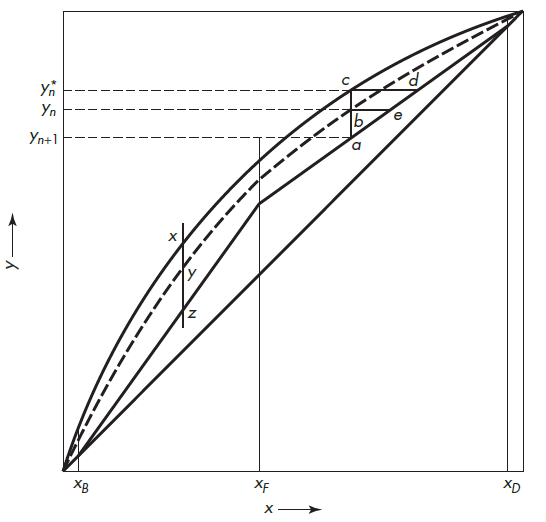
\includegraphics{img/destilacion/EficienciaMurphree_Destilacion.PNG}
    \caption{Uso de la eficiencia de Murphree en un diagrama $xy$. La línea de trazos discontinuos es la curva de equilibrio efectiva, $y'_e$, contra $x_e$ para $\eta_M = 0.60$ $ba/ca = yz/xz = 0.60$.}
    \label{fig:EficienciaMurphree_Destilacion}
\end{figure}

Observe que la posición de la curva $y'_e$ contra $x_e$ depende tanto de la línea de operación como de la verdadera curva de equilibrio. Una vez representada en forma gráfica la curva de equilibrio efectiva, se realiza la habitual construcción de escalones y se determina el número de platos reales. El hervidor no está sometido a la reducción por efecto de la eficiencia de los platos, y se utiliza la verdadera curva de equilibrio para el último escalón en la sección de agotamiento.



\subsection{Método Ponchon-Savarit}

\subsubsection{Balance de Energía}

En las secciones anteriores, se analizaron los casos considerando que se cumple el principio de flujos molares constantes que considera que las capacidades caloríficas de los compuestos son constantes y que los calores latentes también son constantes e iguales entre sí. Estos supuestos son extremadamente útiles ya que permite aplicar un método geométrico simple (método McCabe-Thiele) para conocer la evolución de la concentración de los compuestos a lo largo de la torre de destilación y, si bien existen rara vez todos estos supuestos se cumplen en condiciones industriales, a menudo proporciona un buen punto de partida para el diseño de la columna en sí. 

\begin{figure}[H]
    \centering
    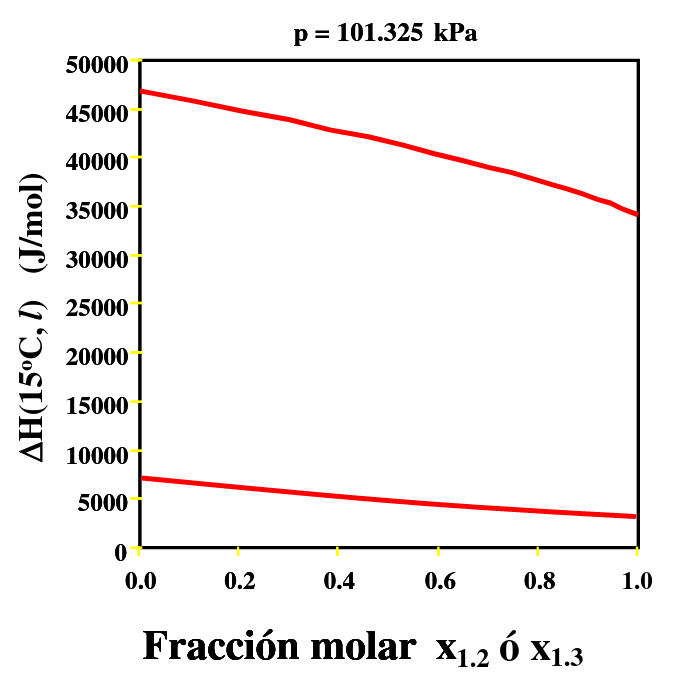
\includegraphics[width = 8cm]{img/destilacion/EntalpiaComposicion.png}
    \caption{Diagrama de Entalpía composición para un mezcla binaria cualquiera}
    \label{fig:DiagramaEntalpiaComposicion}
\end{figure}

Al levantar estos supuestos, los cálculos alrededor de la columna se vuelven tediosos y en muchos casos complejos de resolver. Sin embargo, a lo largo de los años, se han desarrollado métodos que simplifican estos cálculos para algunas situaciones, este es el caso del método gráfico desarrollado por Ruhemann, Ponchon y Savarit para mezclas binarias, que utiliza el gráfico de Entalpía - Composición. Un ejemplo típico de este gráfico es el mostrado en la Figura \ref{fig:DiagramaEntalpiaComposicion}.

\begin{figure}
    \centering
    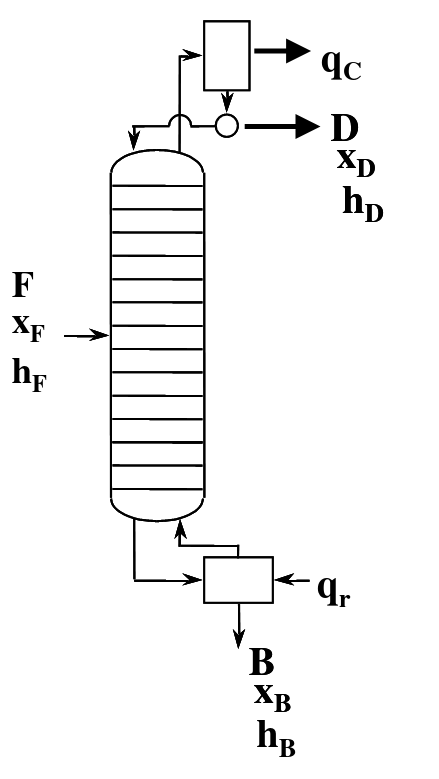
\includegraphics[width=5cm]{img/destilacion/ColumnaDestilacionPonchon.png}
    \caption{Esquema de una columan de Destilacion considerando la energía entregada y retirada por el condensador y hervidor}
    \label{fig:ColumnaDestilacionPonchon}
\end{figure}

En una columna de destilación típica mostrada en la Figura \ref{fig:ColumnaDestilacionPonchon} se alimenta con un flujo molar de F con una composición $x_F$, con un producto destilado $D$ con una composición de $x_D$ y un producto de cola $B$ con una composición de $x_B$. En este caso, la enumeración parte desde arriba de la columna y el subíndice $n$ es utilizado para la zona de rectificicación y $m$ para la zona de agotamiento. 

Si consideramos la columna completa, tenemos que los balances que se pueden plantear son los siguientes:

\textbf{Balance de materia global:}
\begin{equation}
    \label{eq:PonchonSavarit_16}
    F = D + B
\end{equation}

\textbf{Balance de materia del compuesto A:}
\begin{equation}
    \label{eq:PonchonSavarit_17}
    F x_F = D x_D + B x_B
\end{equation}

\textbf{Balance de energía:}
\begin{equation}
    \label{eq:PonchonSavarit_18}
    F h_F + q_r = D h_D + B h_B + q_c
\end{equation}

donde $h_F$, $h_D$ y $h_B$ corresponden a las entalpías líquidas de las corrientes de alimentación, destilado y producto de cola, respectivamente. Y los términos $q_c$ y $q_r$ corresponden a las energías retiradas y entregadas en el condensador y hervidor, respectivamente. 

Con ello, de la combinación de las ecuación \ref{eq:PonchonSavarit_16} y \ref{eq:PonchonSavarit_17} es posible obtener que:

\begin{equation}
    \label{eq:PonchonSavarit_19}
    \frac{D}{B} = \frac{x_F - x_B}{x_D - x_F}
\end{equation}

y de la combinación de la ecuación \ref{eq:PonchonSavarit_16} y \ref{eq:PonchonSavarit_18} y si definimos, el término $h_D + q_c/D$ como $Q_c$ y el término $h_B - q_r/B$ como $Q_r$  obtenemos que:

\begin{equation}
    \label{eq:PonchonSavarit_20}
    \frac{D}{B} = \frac{h_F - Q_r}{Q_c - h_F}
\end{equation}

Con ello, tenemos que la línea de operación global de la columna de operación pasa por los puntos ($x_B$, $Q_r$), ($x_F$, $h_F$) y ($x_D$, $Q_c$).

En en caso de la zona de rectificación los balances son:

\textbf{Balance de materia global:}
\begin{equation*}
    V_n = L_{n+1} + D
\end{equation*}

o, 

\begin{equation}
    \label{eq:PonchonSavarit_1}
    V_n - L_{n+1} = D
\end{equation}


\textbf{Balance de materia del compuesto A:}
\begin{equation*}
    V_n  y_n= L_{n+1} x_{n+1} + D x_D
\end{equation*}

o, 

\begin{equation*}
    \label{eq:PonchonSavarit_2}
    V_n  y_n - L_{n+1} x_{n+1} = D x_D
\end{equation*}

\textbf{Balance de Energía:}
\begin{equation*}
    V_n  H_n= L_{n+1} h_{n+1} + D h_D + q_C
\end{equation*}

o, 

\begin{equation}
    \label{eq:PonchonSavarit_3}
    V_n  H_n - L_{n+1} h_{n+1} = D h_D + q_C
\end{equation}

donde los términos $H$ y $h$ corresponden a las entalpías de las corrientes de vapor y líquido, respectivamente. Y el término $q_C$ corresponde al calor removido por el condensador en la zona superior de la columna.

Si el término $h_D + q_C/D$ de la ecuación \ref{eq:PonchonSavarit_3} lo definimos como $Q_C$ entonces, la ecuacion \ref{eq:PonchonSavarit_3} se puede reescribir de la siguiente manera:

\begin{equation}
    \label{eq:PonchonSavarit_4}
    V_n H_n - L_{n+1} h_{n+1} = DQ_C
\end{equation}

Adicionalmente, tenemos que de las ecuaciones \ref{eq:PonchonSavarit_1} y \ref{eq:PonchonSavarit_2} es posible obtener lo siguiente:

\begin{equation}
    \label{eq:PonchonSavarit_5}
    \frac{L_{n+1}}{D} = \frac{x_D - y_n}{y_n - x_{n+1}}
\end{equation}

y de las ecuaciones \ref{eq:PonchonSavarit_1} y \ref{eq:PonchonSavarit_4} obtenemos:

\begin{equation}
    \label{eq:PonchonSavarit_6}
    \frac{L_{n+1}}{D} = \frac{Q_c - H_n}{H_n - h_{n+1}}
\end{equation}

y si combinamos las ecuaciones \ref{eq:PonchonSavarit_5} y \ref{eq:PonchonSavarit_6}, obtenemos lo siguiente:

\begin{equation}
    \label{eq:PonchonSavarit_7}
    \frac{Q_c - H_n}{H_n - h_{n+1}} = \frac{x_D - y_n}{y_n - x_{n+1}}
\end{equation}

y haciendo un reordenamiento de la ecuación \ref{eq:PonchonSavarit_7} podemos llegar a la siguiente ecuación:

\begin{equation}
    \label{eq:PonchonSavarit_8}
    y_n = \left[ \frac{Q_c - H_n}{Q_c - h_{n+1}} \right] x_{n+1} + \left[ \frac{H_n - h_{n+1}}{Q_c - h_{n+1}} \right] x_D
\end{equation}

La ecuación \ref{eq:PonchonSavarit_8} representa cualquier línea de operacion de la zona de rectificación que relaciona el vapor que asciende por la columna en dicha zona y el líquido que va desciendo por la columna en la zona de rectificación. Desde la ecuación \ref{eq:PonchonSavarit_7} es posible ver que todas las líneas de operación en la zona de rectificación pasan por un punto en común en la coordenada ($x_D$, $Q_c$).

De manera análoga, en la zona de agotamiento es posible plantear los siguientes balances:

\textbf{Balance de materia global:}
\begin{equation}
    \label{eq:PonchonSavarit_9}
    L_{m-1} = V_m + B
\end{equation}

\textbf{Balance de materia del compuesto A:}
\begin{equation}
    \label{eq:PonchonSavarit_10}
    L_{m-1}x_{m-1}= V_m y_m + B x_B
\end{equation}

\textbf{Balance de Energía:}
\begin{equation}
    \label{eq:PonchonSavarit_11}
    L_{m-1} h_{m-1} + q_r= V_m H_m + B h_B
\end{equation}

DOnde el término $q_r$ es el calor entregado por el hervidor. Y si de la ecuación \ref{eq:PonchonSavarit_11} definimos el término $h_B - q_r/B$ como $Q_r$ entonces:

\begin{equation}
    \label{eq:PonchonSavarit_12}
    L_{m-1} h_{m-1}= V_m H_m + B Q_r
\end{equation}

Y haciendo la misma lógica que se hizo en la zona de rectificación, tenemos que:

\begin{equation}
    \label{eq:PonchonSavarit_13}
    \frac{L_{m-1}}{B} = \frac{x_B-y_m}{x_{m-1} - y_m}
\end{equation}

y,

\begin{equation}
    \label{eq:PonchonSavarit_14}
    \frac{L_{m-1}}{B} = \frac{Q_r - H_m}{h_{m-1} - H_m}
\end{equation}

Y si igualamos ambos términos:

\begin{equation}
    \label{eq:PonchonSavarit_15}
    \frac{Q_r - H_m}{h_{m-1} - H_m} = \frac{x_B-y_m}{x_{m-1} - y_m}
\end{equation}

Con ello, tenemos que la ecuación \ref{eq:PonchonSavarit_15} representa cualquier línea de operación de la zona de agotamiento y que todas estas líneas de operación pasan por un punto en común en la coordenada ($x_B$, $Q_r$).

\subsubsection{Determinación del número de platos de platos en un diagrama de Entalpía - Composición}

Para determinar el número de platos de una columna de destilación utilizando el método de Ponchon Savarit, es necesario conocer los puntos ($x_B$, $Q_r$), ($x_F$, $h_F$) y ($x_D$, $Q_c$). Con estos tres puntos es posible trazar la línea de operación en una columan de destilación utilizando el diagrama de Entalpía - Composición (Figura \ref{fig:MetodoPonchonSavarit_1}).

\begin{figure}
    \centering
    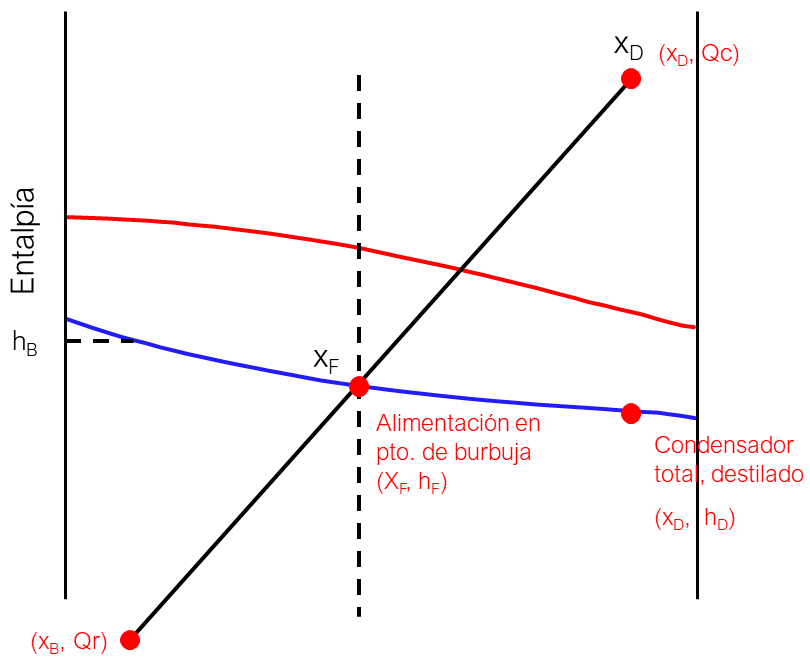
\includegraphics[width=9cm]{img/destilacion/PonchonSavaritLineaOperacion.png}
    \caption{Línea de Operación utilizando el Método Ponchon Savarit}
    \label{fig:MetodoPonchonSavarit_1}
\end{figure}

Una vez trazada esa línea de operación del sistema completo utilizando los puntos de apoyos ($x_B$, $Q_r$) y ($x_D$, $Q_c$) es posible construirlos los escalones en el diagrama permitiendo visualizar las corrientes que se van cruzando en el sistema y las corrientes que están equilibrio fisicoquímico. El punto de apoyo ($x_B$, $Q_r$) lo utilizado para la sección de agotamiento y el punto ($x_D$, $Q_c$) lo utilizamos para la sección de rectificación y con ello se puede obtener la Figura \ref{fig:MetodoPonchonNroPlatos} es posible determinar el número de platos que requiere el sistema considerando el balance de energía del sistema.

\begin{figure}
    \centering
    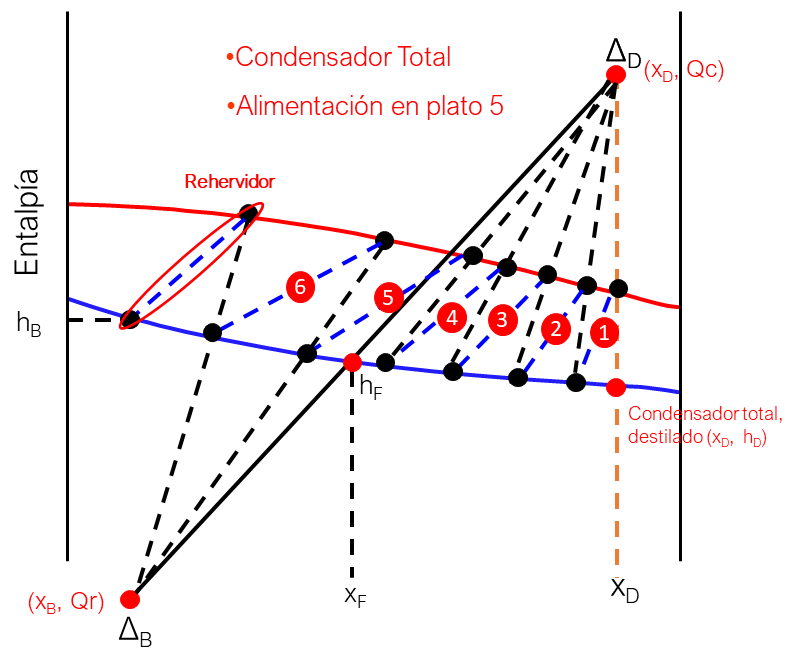
\includegraphics[width=8cm]{img/destilacion/PonchonSavaritNroPlatos.png}
    \caption{Método Ponchon Savarit para determinar el número de platos considerando un condensador total en la columna}
    \label{fig:MetodoPonchonNroPlatos}
\end{figure}

\newpage

\subsubsection{Reflujo Mínimo en un diagrama de Entalpía - Composición}

Sabemos que en el sistema real, en la zona de rectificación, el punto de apoyo es ($x_D$, $Q_c$). Sin embargo, si vamos reduciendo el punto $Q_c$ tenemos que vamos aumentando en número de platos necesarios para destilar el sistema. Y cuando alcanzamos el punto de quiebre de reflujo mínimo ($Q_{c \textrm{, min}}$), tenemos que existen infinitos platos de destilación. Esto generalmente, ocurre en la isoterma del punto de la alimentación, cuando se realiza la proyección de la isoterma (o línea de enlace) desde la alimentación, cuando alcanza al punto de la composición del destilado decimos que alcanzamos el reflujo mínimo, tal como se observa en la Figura \ref{fig:PonchonSavaritReflujoMinimo}. 

\begin{figure}[H]
    \centering
    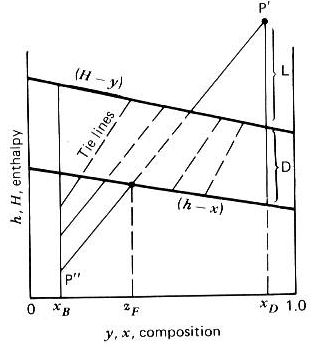
\includegraphics[width=6cm]{img/destilacion/PonchonSavaritReflujoMinimo.png}
    \caption{Método Ponchon Savarit para determinar el reflujo mínimo siguiendo la isoterma o linea de enlace desde la alimentación}
    \label{fig:PonchonSavaritReflujoMinimo}
\end{figure}



\chapter{Separación Líquido-Líquido}

\section{Introducción}

Al proceso de separar compuestos desde una mezcla líquida utilizando un solvente (líquido) que tiene afinidad por uno o más componentes de la mezcla se le denomina como extracción líquida-líquida. Y esta operación ha sido ampliamente usada en la producción de combustibles en la industria nuclear y en la separación de hidrocarburos en la industria del petróleo. En esta operación unitaria, es esencial que la mezcla líquida de alimentación y el solvente sean al menos parcialmente miscible y, en esencia, tiene 3 etapas involucradas.

\begin{enumerate}
    \item Poner en contacto íntimo la mezcla de alimentación y el solvente (o disolvente).
    
    \item Separación de los productos en dos fases.
    
    \item Remoción y recuperación del solvente desde cada una de las fases.
\end{enumerate}

Es importante mencionar que es posible combinar las etapas (1) y (2) en un sólo equipo, como lo es una columna de separación continua. 

La extracción líquido-líquido es en muchas manera complementaria a la destilación y es preferible en los siguientes casos:

\begin{itemize}
    \item Cuando la destilación podría requerir una cantidad excesiva de calor, como por ejemplo, cuando las volatilidades relativas son cercanas a la unidad.
    
    \item Cuando la formación de azeotropos limita la pureza que se puede obtener en la destilación.
    
    \item Cuando es necesario evitar el calentamiento de los compuestos, por ejemplo, compuestos aromáticos que son sensibles a la temperatura.
\end{itemize}

En todos los procesos de extracción, una característica importante es la naturaleza selectiva del solvente, en que la separación de los componentes se basa en la diferencia de solubilidad que existe entre los compuestos. 

\section{Equilibrio en Sistemas Ternarios}

En los procesos de extracción líquido-líquido se basa en mezclar compuestos en estado líquido. Esta mezclas pueden generar dos situaciones (Figura \ref{fig:MezclaLiquidoLiquido}). En la Figura \ref{fig:Mezcla_LiquidoLiquido_1} se puede apreciar que cuando los compuestos que se muestran tienen una buena afinidad entre ellos se mezclan completamente formando una única fase y por tanto se dice que los compuestos son \textbf{miscibles}. En contraposición, en la Figura \ref{fig:Mezcla_LiquidoLiquido_2} se puede apreciar que cuando los compuestos no tienen una buena afinidad, se separan en dos fases distinguibles entre sí, a estos compuestos se les denominma compuestos \textbf{inmiscibles}.

\begin{figure}[H]
  \begin{subfigure}[b]{0.45\textwidth}
    \centering
    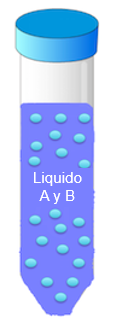
\includegraphics[width=2.5cm]{img/LiquidoLiquido/MezclaLiquidoLiquido_1.PNG}
    \caption{ }
    \label{fig:Mezcla_LiquidoLiquido_1}
  \end{subfigure}
  \hfill
  \begin{subfigure}[b]{0.45\textwidth}
    \centering
    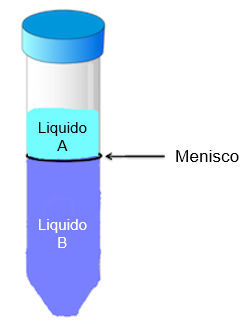
\includegraphics[width=5.3cm]{img/LiquidoLiquido/MezclaLiquidoLiquido_2.PNG}
    \caption{ }
    \label{fig:Mezcla_LiquidoLiquido_2}
  \end{subfigure}
  \caption{Posibles situaciones en una mezcla de dos líquidos: (a) Ambos fluidos son miscibles por lo que se forma una única fase, (b) Ambos fluidos no son miscibles por lo que se forman 2 fases diferentes.}
  \label{fig:MezclaLiquidoLiquido}
\end{figure}

Haciendo provecho de estas dos situaciones lo que hacemos en la extracción líquido-líquido es que a una mezcla binaria de compuestos que son completamente miscibles entre sí se le adiciona un nuevo compuesto que es parcialmente miscible con uno o ambos compuestos. Entonces este compuesto nuevo actua como solvente que arrastra uno de los componente a una fase diferente a la del otro compuesto y con eso es posible realizar la división de estos dos compuestos que originalmente eran totalmente miscibles.

Para representar esta mezcla entre estos 3 compuestos generamente se hace uno de un \textbf{diagrama Ternario}. Estos diagramas ternarios se construyen a partir de las coordenadas cartesianas. Para ello, podemos considerar una mezcla de 3 compuestos A, B y C y su mezcla tiene a\% de A, b\% de B y c\% de C, con ello la representación de esa mezcla en una diagrama cartesiano es:

\begin{figure}[H]
    \centering
    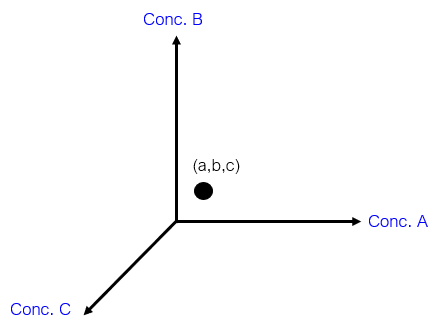
\includegraphics{img/LiquidoLiquido/MezclaTresCompuestos.PNG}
    \caption{Representación en coordenadas cartesianas de una Mezcla ternaria de los compuestos A, B y C}
    \label{fig:MezclaTresCompuestos}
\end{figure}
 
Sin embargo, el punto $(a,b,c)$ de la Figura \ref{fig:MezclaTresCompuestos} está encerrado en el triángulo equilatero formados por los valores máximos que puede tomar la mezcla de estos 3 compuestos:

\begin{figure}[H]
    \centering
    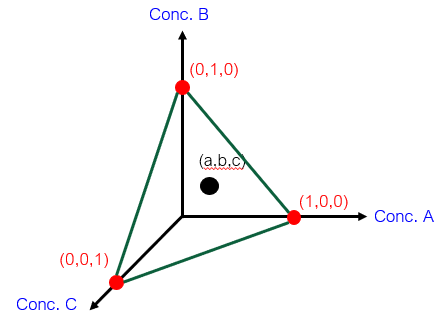
\includegraphics{img/LiquidoLiquido/MezclaTresCompuestos_2.PNG}
    \caption{Representación de los límites de una Mezcla ternaria de los compuestos A, B y C}
    \label{fig:MezclaTresCompuestos_2}
\end{figure}

Este triángulo equilatero lo podemos extraer de las coordenadas cartesianas y obtener este punto $(a,b,c)$ en unas nuevas coordenadas ahora solo considerando el triangulo que rodea al punto.

\begin{figure}[H]
    \centering
    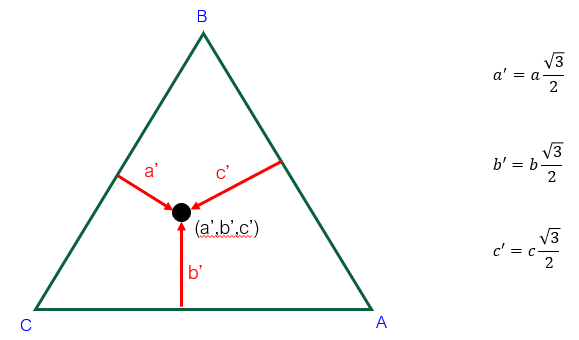
\includegraphics[width = 10cm]{img/LiquidoLiquido/MezclaTresCompuestos_3.PNG}
    \caption{Representación de una Mezcla ternaria de los compuestos A, B y C en coordenas triangulares}
    \label{fig:MezclaTresCompuestos_3}
\end{figure}

A este forma de representar una mezcla ternaria líquida se le conoce como \textbf{Diagrama Ternario}. Entonces en un ejemplo de una mezcla de A al 20\%, B al 40\% y C al 40\%, tenemos que su representación en el diagrama ternario es el siguiente:

\begin{figure}[H]
    \centering
    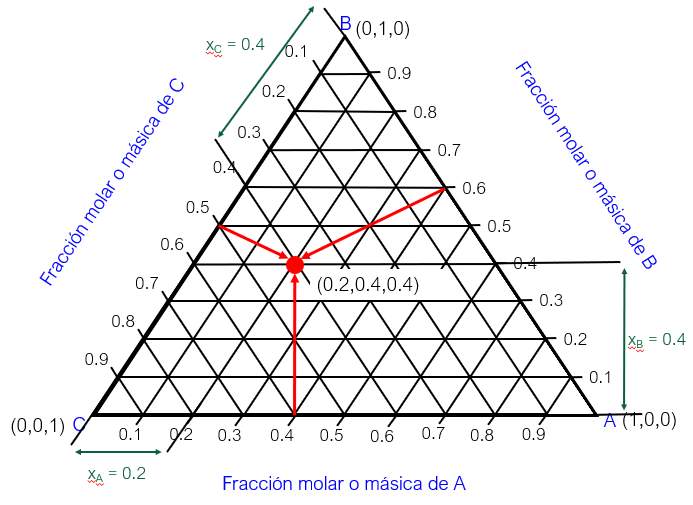
\includegraphics[width = 10cm]{img/LiquidoLiquido/DiagramaTriangular.PNG}
    \caption{Diagrama Ternario para una mezcla A al 20\%, B al 40\% y C al 40\%}
    \label{fig:DiagramaTriangular}
\end{figure}

Haciendo uso de este diagrama triángular es posible hacer la representación de los tipos de mezclas líquido-líquido que se pueden formar. Para ellos, es importante considerar que en la extracción líquido-líquido deseamos que el nuevo solvente añadido al sistema sea al menos parcialmente miscible con uno de los dos otros compuestos y con ello es posible identificar las diferentes regiones que se forman en una mezcla ternaria (Figura \ref{fig:MezclaTernaria})

\begin{figure}
    \centering
    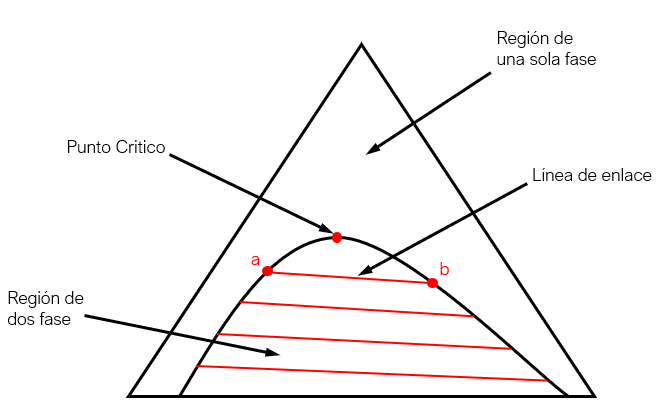
\includegraphics[width = 10cm]{img/LiquidoLiquido/DiagramaTriangular_Puntos.PNG}
    \caption{Diferentes regiones y puntos que se forman en una mezcla ternaria}
    \label{fig:MezclaTernaria}
\end{figure}

Tal como se puede apreciar en la Figura \ref{fig:MezclaTernaria} los puntos $a$ y $b$ se encuentran en equilibrio fisicoquímico y hace referencia a las composiciones que tienen las dos fases que se forman en el sistema cuando estamos en la región de dos fases. 

En consideración de lo anterior podemos tener dos situaciones posibles cuando nos enfretamos a un diagrama ternario de una extracción líquido-líquido:

\begin{itemize}
    \item \textbf{Sistemas Tipo I:} Son aquellos en que en la mezcla ternaria sólo existe un par de líquidos parcialmente miscibles (Figura \ref{fig:LiqLiqSistema_1}).
    
    \item \textbf{Sistema Tipo II:} Son aquellos en que en la mezcla ternaria existen 2 pares de líquidos inmiscibles (Figura \ref{fig:LiqLiqSistema_2}).
\end{itemize}


\begin{figure}[H]
  \begin{subfigure}[b]{0.45\textwidth}
    \centering
    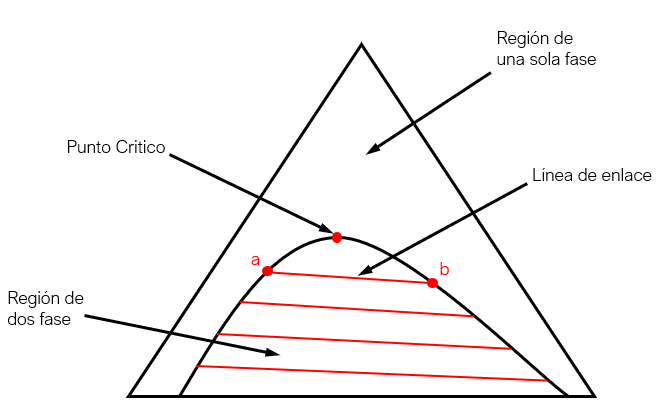
\includegraphics[width=\textwidth]{img/LiquidoLiquido/DiagramaTriangular_Puntos.PNG}
    \caption{ }
    \label{fig:LiqLiqSistema_1}
  \end{subfigure}
  \hfill
  \begin{subfigure}[b]{0.50\textwidth}
    \centering
    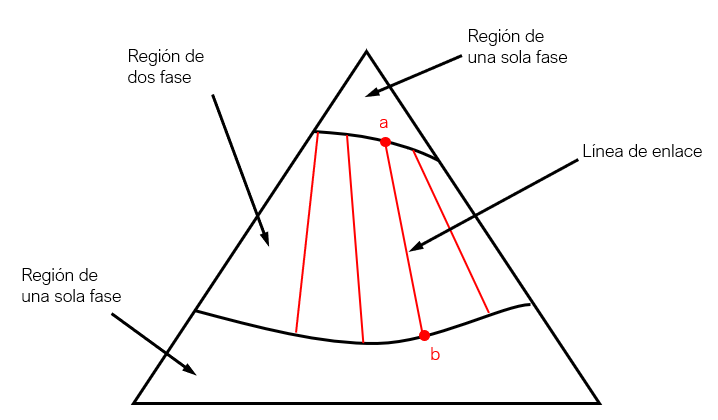
\includegraphics[width=\textwidth]{img/LiquidoLiquido/DiagramaTriangular_Puntos_2.PNG}
    \caption{ }
    \label{fig:LiqLiqSistema_2}
  \end{subfigure}
  \caption{Distintos sistemas que se forman en una mezcla ternaria en una extracción líquido-líquido: (a) Sistema Tipo I, (b) Sistema Tipo II.}
  \label{fig:LiqLiqSistemas}
\end{figure}

Adicional a los diagramas ternarios en un triángulo equilátero es posible trabajar una mezcla ternaría en un triángulo rectangulo con el fin de apoyarnos parcialmente en las coordenadas cartesianas en dos dimensiones. Para ello,  supongamos que tenemos una mezcla de tres compuestos con concentraciones $(a,b,c)$ lo que podemos hacer es construir un triangulo rectangulo apoyado en los ejes $x$ e $y$ de las coordenadas cartesianas, tal como se muestra en la Figura \ref{fig:MezclaLiqLiqTrianguloRectangulo}.

\begin{figure}[H]
    \centering
    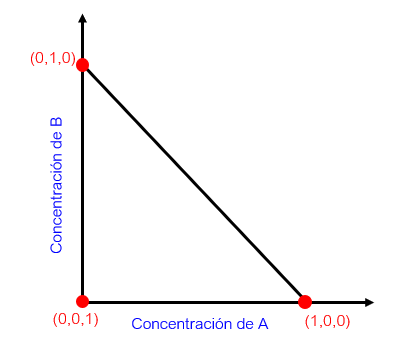
\includegraphics{img/LiquidoLiquido/TrianguloRectangulo.PNG}
    \caption{Diagrama ternario en un triangulo rectangulo}
    \label{fig:MezclaLiqLiqTrianguloRectangulo}
\end{figure}

En la Figura \ref{fig:MezclaLiqLiqTrianguloRectangulo} se puede apreciar los puntos límites de esta mezcla de tres componentes, en donde el punto $(0,0)$ en la coordenada cartesiana en dos dimensiones representa el punto de máxima concentración posible del compuesto C.

Entonces en este diagrama el punto $(a,b,c)$ se representa de la siguiente manera:

\begin{figure}[H]
    \centering
    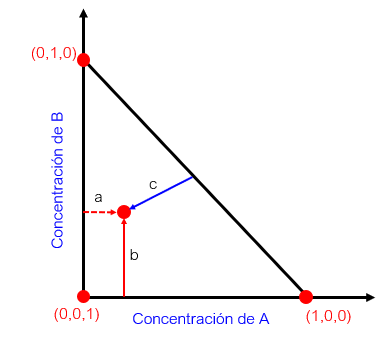
\includegraphics{img/LiquidoLiquido/TrianguloRectangulo_2.PNG}
    \caption{Diagrama ternario en un triangulo rectangulo del punto $(a,b,c)$}
    \label{fig:MezclaLiqLiqTrianguloRectangulo_2}
\end{figure}

Finalmente, es importante mencionar que tanto la representación de triángulo equilátero como triángulo rectangulo son equivalentes, por lo que es posible representar una mezcla ternaria en cualquiera de las dos formas del diagrama ternario, tal como se muestra en la Figura \ref{fig:MezclaLiqLiqTrianguloRectangulo_3}

\begin{figure}[H]
    \centering
    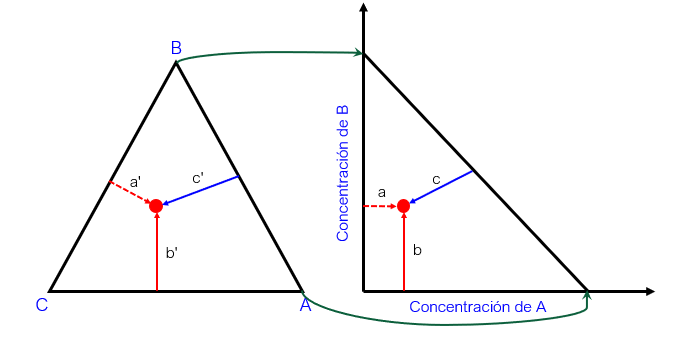
\includegraphics{img/LiquidoLiquido/TrianguloRectangulo_3.PNG}
    \caption{Representación de la mezcla de tres compuestos en el punto $(a,b,c)$ en las dos formas del diagrama ternario}
    \label{fig:MezclaLiqLiqTrianguloRectangulo_3}
\end{figure}

\section{Proceso de Extracción Líquido-Líquido en una etapa}

Consideremos que tenemos una mezcla binaria de compuestos que son totalmente miscibles entre sí, es decir, que solo hay una fase en la mezcla y que a esta solución le añadimos un tercer componente que es parcialmente miscible con uno de los dos componentes de la mezcla binaria original. A este tercer componente se le conoce como \textbf{Solvente} (Figura \ref{fig:MezclaLiqLiqSolvente})

\begin{figure}[H]
    \centering
    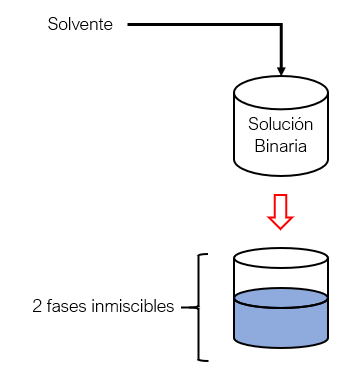
\includegraphics[width =7cm]{img/LiquidoLiquido/MezclaLiqLiqSolvente.PNG}
    \caption{Proceso de mezclar una mezcla binaria totalmente miscible con un tercer compuesto que es parcialmente miscible con uno de los dos compuestos originales}
    \label{fig:MezclaLiqLiqSolvente}
\end{figure}

A esta mezcla resultante que tiene dos fases se le puede hacer pasar por un proceso de separación con el fin de separar las dos fases existentes. Estos dos procesos de combinar la mezcla binaria original con un solvente y posteriomente separar la mezcla en las dos fases se efectua en concreto en dos equipos: un contactador y un separador, respectivamente (Figura \ref{fig:ExtraccionLiqLiq_1Etapa}).

\begin{figure}[H]
    \centering
    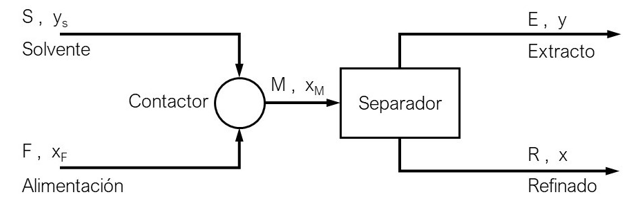
\includegraphics[width =12cm]{img/LiquidoLiquido/ExtracionLiqLiq_1Etapa.PNG}
    \caption{Proceso de Extracción Líquido-Líquido en una etapa}
    \label{fig:ExtraccionLiqLiq_1Etapa}
\end{figure}

Es importante mencionar que las corrientes que salen del separador son dos:
\begin{itemize}
    \item \textbf{Extracto:} La fase líquida que contiene la mayor concentración de solvente
    
    \item \textbf{Refinado:} La otra fase líquida, que contiene una concentración pequeña de solvente 
\end{itemize}

En este estos equipos es posible plantear los siguientes balances:

\textbf{Balance de Materia Global:}

\begin{equation}
    \label{eq:Extraccion_LiqLiq_1}
    F + S = M = E + R
\end{equation}

\textbf{Balance de Materia del compuesto A:}

\begin{equation}
    \label{eq:Extraccion_LiqLiq_2}
    F x_{A,F} + S y_{A,S} = M x_{A,M} = E y_{A,E} + R x_{A,R}
\end{equation}

Es importante notar que las composiciones del Extracto y Refinado están en \textbf{Equilibrio Fisicoquímico}. Considernado lo anterior y haciendo uno de un diagrama ternario de triángulo rectángulo es posible representar los puntos vistos en el balance (Figura \ref{fig:ExtraccionLiqLiq_1Etapa_2})

\begin{figure}[H]
    \centering
    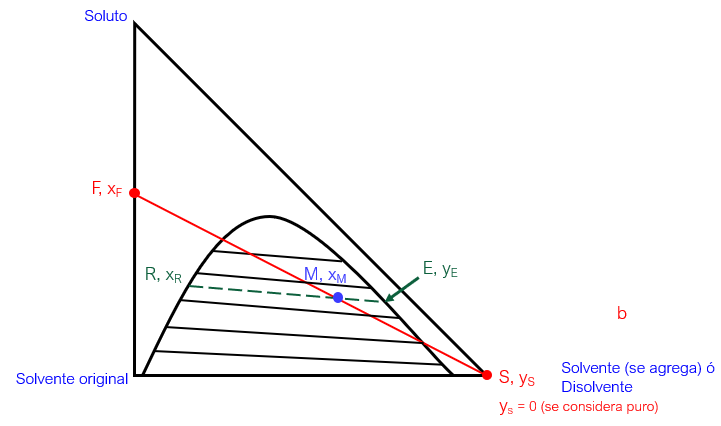
\includegraphics[width =10.5cm]{img/LiquidoLiquido/ExtracionLiqLiq_1Etapa_2.PNG}
    \caption{Representación de un extracción Líquido-Líquido en una sola etapa}
    \label{fig:ExtraccionLiqLiq_1Etapa_2}
\end{figure}

\subsection{Coeficiente de Distribución y Selectividad}

Al igual que ocurre en una mezcla líquido-vapor, en una mezcla líquido-líquido que se forma en un proceso de extracción estamos haciendo uso de que los compuestos al tener el suficiente tiempo alcanzan eventualmente el equilibrio fisicoquímico. 

Este equilibrio que se forma entre la fase de extracto y la de refinado, tal como se vio en el Capítulo 1, está están relacionadas a través del valor K. Y en el caso de una mezcla líquido-líquido este valor K viene dado por la siguiente expresión:

\begin{equation}
    \label{eq:Extraccion_LiqLiq_3}
    K_{i} = \frac{x_{i,E}}{x_{i,R}}
\end{equation}

donde los términos $x_{i,E}$ y $x_{i,R}$ son las concentraciones del compuesto $i$ en el Extracto y Refinado, respectivamente. A este término $K$ en la extracción líquido-líqudio se le denomina \textbf{Coeficiente de Distribución} y se representa con $K_{D,i}$ o $D_i$. Este término hace alución de cómo se distribuye el compuesto $i$ en las dos fases inmiscibles que se forma en la mezcla ternaria.


En conjunto con este coeficiente de distribución, es posible construir un término simil al coeficiente de volatilidad pero aplicado a mezclas líquidas. Esta expresión en mezcla líquidas se le conoce como \textbf{Selectividad} y se expresa de la siguiente manera:

\begin{equation}
    \label{eq:Extraccion_LiqLiq_4}
    \beta_{i,j} = \frac{K_{D,i}}{K_{D,j}} = \frac{\sfrac{x_{i,E}}{x_{i,R}}}{\sfrac{x_{j,E}}{x_{j,R}}}
\end{equation}

\section{Extracción Líquido-Líquido en múltiples etapas}

Al igual que ocurría con la destilación flash, en la extracción líquido-líquido en una etapa estamos limitados en la pureza que podemos llegar a obtener en el equipo. Debido a estos es que en la industría se desarrollaron diferentes configuraciones para la extracción multiples etapas:

\begin{enumerate}
    \item \textbf{Configuración Co-Corriente:} Ambos flujos de extracto y refinado se vuelven a ingresar una etapa de extracción líquido-líquido, con el fin de asegurar la formación del equilibrio fisicoquímico.
    
    \item \textbf{Configuración Flujos Cruzados:} Una de las corrientes (generalmente la de refinado) se reingresa a una nueva estapa de extracción y se enfrenta a una nueva corriente de solvente.
    
    \item \textbf{Configuración Contracorriente:} El flujo de alimentación y el de solvente se alimentan en direcciones opuestas de ambos extremos de una serie de extractores líquido-líquido en seríe.
\end{enumerate}

\subsection{Configuración Co-Corriente}

La primera aproximación realizada a la extracción multi-etapa líquido-líquido es la configuración co-corriente. En esta configuración se colocan equipos de extracción en serie y las corrientes de salida de las etapas se vuelven a ingresar a la etapa siguiente (ver Figura \ref{fig:ExtraccionLiqLiqCocorriente}).

\begin{figure}[H]
    \centering
    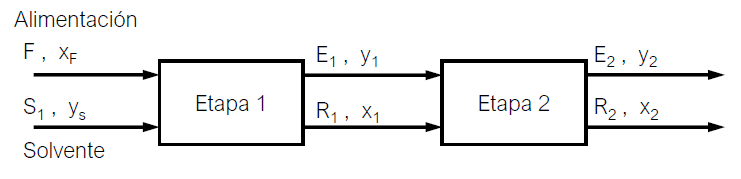
\includegraphics{img/LiquidoLiquido/ExtracionLiqLiqCoCorriente.PNG}
    \caption{Ejemplo de una configuración Co-Corriente de 2 etapas}
    \label{fig:ExtraccionLiqLiqCocorriente}
\end{figure}

Si analizamos la primara etapa obtendríamos los siguientes balances: 

\textbf{Balance Global de Matería:}
\begin{equation}
    \label{eq:ExtraccionLiqLiqCocorriente_1}
    F + S_1 = M_1 = E_1 + R_1
\end{equation}

\textbf{Balance de Materia del compuesto A:}
\begin{equation}
    \label{eq:ExtraccionLiqLiqCocorriente_2}
    F x_{A.F} + S_1 y_{A,S} = M_1 x_{A,1,M} = E_1 y_{A,1} + R_1 x_{A,1}
\end{equation}

Con este balance planteado tenemos que existe un punto de mezcla $M_1$ que se genera al juntar la corriente de alimentación y el solvente. Este punto de mezcla si cae dentro de la fase inmiscible es posible lleva a cabo la extracción líquido-líquido, logrando obtener un extracto ($E_1$) y un refinado ($R_1$), tal como se muestra en la Figura \ref{fig:ExtraccionLiqLiqCocorriente_2}

\begin{figure}[H]
    \centering
    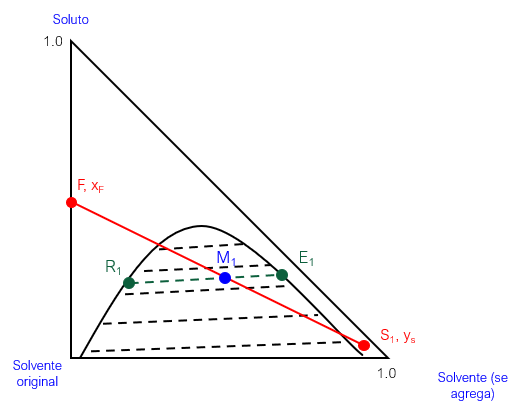
\includegraphics{img/LiquidoLiquido/ExtracionLiqLiqCoCorriente_2.PNG}
    \caption{Representación de una Extracción Líquido-Líquido de la primera etapa de una extracción a Co-Corriente}
    \label{fig:ExtraccionLiqLiqCocorriente_2}
\end{figure}

Ahora si hacemos el balance de materia en la segunda etapa de proceso, tenemos lo siguiente:

\textbf{Balance Global de Matería:}
\begin{equation}
    \label{eq:ExtraccionLiqLiqCocorriente_3}
    E_1 + R_1 = M_2 = E_2 + R_2
\end{equation}

\textbf{Balance de Materia del compuesto A:}
\begin{equation}
    \label{eq:ExtraccionLiqLiqCocorriente_4}
    E_1 y_{A,1} + R_1 x_{A,1} = M_2 x_{A,2,M} = E_2 y_{A,2} + R_2 x_{A,2}
\end{equation}

Sin embargo, si los puntos $E_1$ y $R_1$ originalmente aparecen debido a que existió una mezcla $M_1$. Como los puntos $E_1$ y $R_1$ se vuelven a enfrentar en la etapa 2 tenemos que los sistemas ya se encuentran en la transición al equilibrio fisicoquímico, por lo que la línea de operación de la etapa 2 y la línea de equilibrio coinciden por lo tanto tenemos un sistema que no tiene fuerza motriz para realizar un cambio en la composición de los flujos de salida, por lo tanto, $M_1 = M_2$ y por consiguiente, $R_2$ y $E_2$ son iguales a los puntos de extracto y refinado de la etapa 1.

\subsection{Configuraciónn Flujos Cruzados}

\subsubsection{Extracción en dos etapas}

Considerando que la extracción en la configuración a Co-Corriente no genera la fuerza motriz necesaria para aumentar la pureza de los compuestos que tenemos en la mezcla de alimentación, una alternativa es sólo continuar operando con uno de los flujos de salida y el otro se "descarta" (generalmente se utiliza como solvente otra líena de extracción líquido-líquido). Un ejemplo de esta configuración es la presentada en la Figura \ref{fig:ExtraccionLiqLiqCruzado_1}, en donde el refinado de la etapa 1 se utiliza como alimentación para la etapa 2 y este refinado se enfrenta a un solvente $S_2$.

\begin{figure}
    \centering
    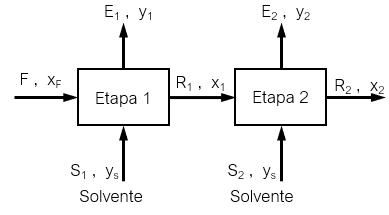
\includegraphics{img/LiquidoLiquido/ExtracionLiqLiqCruzado_1.PNG}
    \caption{Ejemplo de una configuración a flujos cruzados con 2 etapas}
    \label{fig:ExtraccionLiqLiqCruzado_1}
\end{figure}

Haciendo el balance de materia de la representación de la Figura \ref{fig:ExtraccionLiqLiqCruzado_1}, obtenemos lo siguiente:

\textbf{Balance Global de Matería:}
\begin{equation}
    \label{eq:ExtraccionLiqLiqCruzado_1}
    F + S_1 = M_1 = E_1 + R_1
\end{equation}

\textbf{Balance de Materia del compuesto A:}
\begin{equation}
    \label{eq:ExtraccionLiqLiqCruzado_2}
    F x_{A.F} + S_1 y_{A,S} = M_1 x_{A,1,M} = E_1 y_{A,1} + R_1 x_{A,1}
\end{equation}

Este balance de matería representa que el punto $M_1$ es común a la línea que une los puntos de alimentación ($F$) y el solvente ($S_1$) y la línea que conecta los puntos del refinado ($R_1$) y extracto ($E_1$). Tal como se muestra en la Figura \ref{fig:ExtraccionLiqLiqCruzado_2}

\begin{figure}
    \centering
    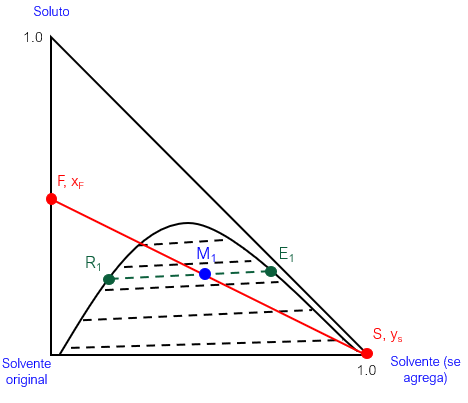
\includegraphics{img/LiquidoLiquido/ExtracionLiqLiqCruzado_2.PNG}
    \caption{Representación de una Extracción Líquido-Líquido de la primera etapa de una extracción a flujo cruzado.}
    \label{fig:ExtraccionLiqLiqCruzado_2}
\end{figure}

Es importante recordar que los puntos $R_1$ y $E_1$ se le damos el suficiente tiempo, están en equilibrio fisicoquímico, por eso esos puntos están en la línea de enlace que conecta las dos fases inmiscibles que se forma en la mezcla ternaria.

Con respecto a la etapa 2, tenemos que el balance es el siguiente:

\textbf{Balance Global de Matería:}
\begin{equation}
    \label{eq:ExtraccionLiqLiqCruzado_3}
    R_1 + S_2 = M_2 = E_2 + R_2
\end{equation}

\textbf{Balance de Materia del compuesto A:}
\begin{equation}
    \label{eq:ExtraccionLiqLiqCruzado_4}
   R_1 x_{A,1} + S_2 y_{A,2} = M_2 x_{A,2,M} = E_2 y_{A,2} + R_2 x_{A,2}
\end{equation}

Al analizar las ecuaciones \ref{eq:ExtraccionLiqLiqCruzado_3} y \ref{eq:ExtraccionLiqLiqCruzado_4} podemos apreciar que el punto de mezcla $M_2$ es común a la línea que conecta los puntos $R_1$ y $S_2$ y la línea que conecta $E_2$ y $R_2$, tal como se muestra en la Figura \ref{fig:ExtraccionLiqLiqCruzado_3}.

\begin{figure}
    \centering
    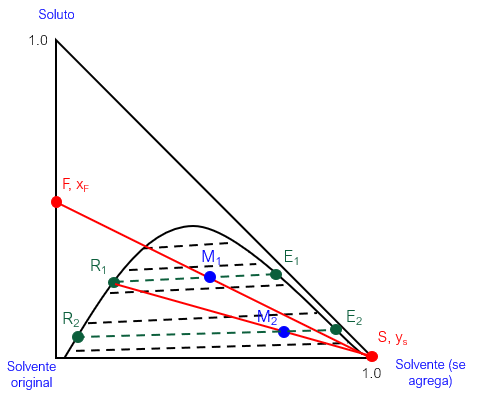
\includegraphics{img/LiquidoLiquido/ExtracionLiqLiqCruzado_3.PNG}
    \caption{Representación de una Extracción Líquido-Líquido de una extracción a flujo cruzado de 2 etapas.}
    \label{fig:ExtraccionLiqLiqCruzado_3}
\end{figure}

En contraposición de lo que ocurren en la configuración Co-Corriente, en esta configuración tenemos que los flujos que se cruzan generan un nuevo punto de mezcla $M_2$ lo que le permite al sistema alcanzar un nuevo punto de extracto y refinado, que en este caso es más puro que lo que se obtuvo en la etapa anterior.

\subsubsection{Extracción Múltiples Etapas a Configuración a Flujo Cruzado}

La conformación más simple de una configuración a Flujo Cruzado es la presentada en la Figura \ref{fig:ExtraccionLiqLiqCruzado_4}. En donde el refinado viaja a lo largo de los equipos de extracción en serie y los flujos de extracto se "desecha" de esta línea de proceso. 

En esta configuración los balances que se pueden plantear en la etapa $n$ son:

\textbf{Balance Global de Matería:}
\begin{equation}
    \label{eq:ExtraccionLiqLiqCruzado_5}
    R_{n-1} + S_n = M_n = R_n + E_n
\end{equation}

\textbf{Balance de Materia del compuesto A:}
\begin{equation}
    \label{eq:ExtraccionLiqLiqCruzado_6}
   R_{n-1} x_{A,n-1} + S_n y_{A,n} = M_n x_{A,n,M} = E_n y_{A,n} + R_n x_{A,n}
\end{equation}

\begin{figure}[H]
    \centering
    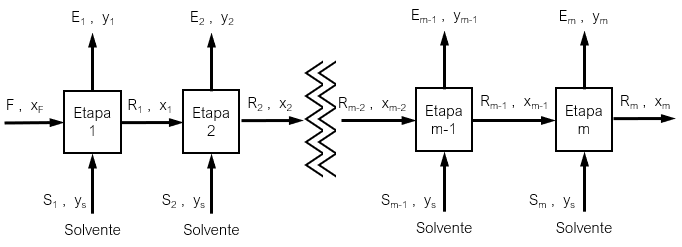
\includegraphics{img/LiquidoLiquido/ExtracionLiqLiqCruzado_4.PNG}
    \caption{Representación de una Extracción Líquido-Líquido de una extracción a flujo cruzado multiples etapas.}
    \label{fig:ExtraccionLiqLiqCruzado_4}
\end{figure}

En las configuraciones a Flujos Cruzados, tenemos que en general el flujo que se "desecha" se aprovecha en otra línea de proceso ya sea como extracto o refinado tal como se presenta en la Figura \ref{fig:ExtraccionLiqLiqCruzado_5} y \ref{fig:ExtraccionLiqLiqCruzado_6}

\begin{figure}[H]
    \centering
    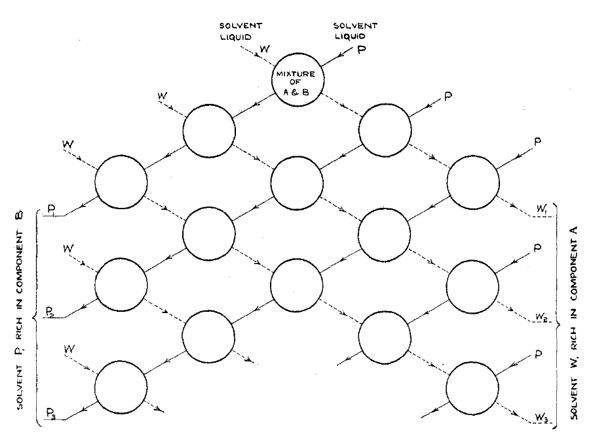
\includegraphics{img/LiquidoLiquido/ExtracionLiqLiqCruzado_5.PNG}
    \caption{Diagrama de una línea de extracción a Flujo Cruzado.}
    \label{fig:ExtraccionLiqLiqCruzado_5}
\end{figure}

\begin{figure}[H]
    \centering
    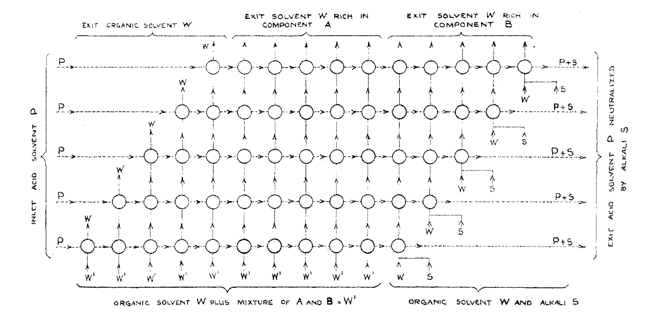
\includegraphics{img/LiquidoLiquido/ExtracionLiqLiqCruzado_6.PNG}
    \caption{Diagrama de múltiples líneas de extracción a Flujo Cruzado.}
    \label{fig:ExtraccionLiqLiqCruzado_6}
\end{figure}

\subsection{Configuración Contracorriente}

En esta configuración, la alimentación y el solvente que se agrega se ingresan en posición opuesta del equipo y los flujos van en direcciones opuestas entre sí, tal como se aprecia en la Figura \ref{fig:ExtraccionLiqLiqContraCorriente_1}

\begin{figure}[H]
    \centering
    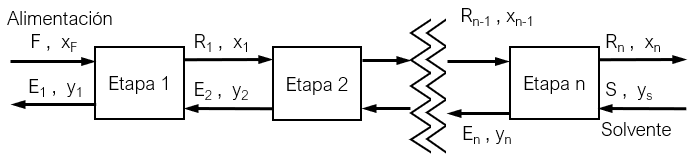
\includegraphics{img/LiquidoLiquido/ExtraccionLiqLiq_ContraCorriente_1.PNG}
    \caption{Ejemplo del proceso de extracción líquido-líquido en su configuración a ContraCorriente.}
    \label{fig:ExtraccionLiqLiqContraCorriente_1}
\end{figure}

En esta configuración lo primero que debemos hacer para entender lo que está ocurriendo al interior de cada una de estás etapas, es plantear el balance completo de todo el sistema, para ello hacemos la envolvente respectiva que considera sólo los flujos que ingresan y salen del sistema en su completo (Figura \ref{fig:ExtraccionLiqLiqContraCorriente_2})

\begin{figure}[H]
    \centering
    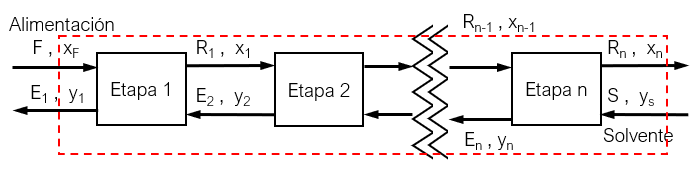
\includegraphics{img/LiquidoLiquido/ExtraccionLiqLiq_ContraCorriente_2.PNG}
    \caption{Envolvente Global para la extracción líquido-líquido en su configuración a ContraCorriente.}
    \label{fig:ExtraccionLiqLiqContraCorriente_2}
\end{figure}

Tal como se puede apreciar en la Figura \ref{fig:ExtraccionLiqLiqContraCorriente_2}, los balances que podemos plantear son los siguientes:

\textbf{Balance Global de Matería:}
\begin{equation}
    \label{eq:ExtraccionLiqLiqContracorriente_1}
    F + S = M = R_n + E_1 
\end{equation}

\textbf{Balance de Materia del compuesto A:}
\begin{equation}
    \label{eq:ExtraccionLiqLiqContracorriente_2}
   F x_{A,F} + S y_{A,S} = M x_{A,M} = R_n x_{A,n} + E_1 y_{A,1}
\end{equation}

En las ecuaciones \ref{eq:ExtraccionLiqLiqContracorriente_1} y \ref{eq:ExtraccionLiqLiqContracorriente_2} se puede apreciar que el punto $M$ representa el punto de mezcla global del sistema y está en la intercepción de las líneas que unen los puntos $F$ y $S$ y la línea que une los puntos $E_1$ y $R_n$, tal como se aprecia en la Figura \ref{fig:ExtraccionLiqLiqContraCorriente_3}

\begin{figure}[H]
    \centering
    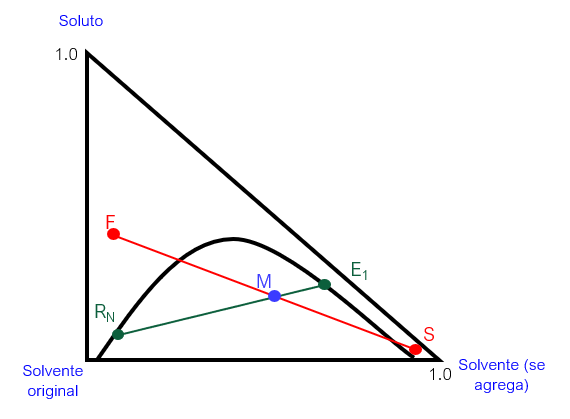
\includegraphics{img/LiquidoLiquido/ExtraccionLiqLiq_ContraCorriente_3.PNG}
    \caption{Identificación del punto de mezcla global $M$ en un Diagrama ternario de una extracción líquido-líquido en configuración Contracorriente.}
    \label{fig:ExtraccionLiqLiqContraCorriente_3}
\end{figure}

En esta configuración, el punto $M$ se puede localizar aplicando las ecuaciones de balance, obteniendo lo siguiente:

\begin{equation}
    \label{eq:ExtraccionLiqLiqContracorriente_3}
    x_M = \frac{F x_{A,F}+S y_{A,S}}{M} = \frac{F x_{A,F}+S y_{A,S}}{F+S}
\end{equation}

y por regla de palanca, tenemos que:

\begin{equation}
    \label{eq:ExtraccionLiqLiqContracorriente_4}
    \frac{S}{F} = \frac{\overline{FM}}{\overline{SM}}
\end{equation}

Sin embargo, si reorganizamos la ecuación \ref{eq:ExtraccionLiqLiqContracorriente_1} agrupando los términos que ingresan y salen desde el mismo lado de cada etapa, tenemos que existe un delta de flujo $\Delta$ que es constante tanto en la primera etapa como en la última etapa, debido a que en la extracción líquido-líquido no exite acumulación de materia en ninguna de las etapas presentes en el sistema. Con ello la ecuación \ref{eq:ExtraccionLiqLiqContracorriente_1} se convierte en:

\begin{equation}
    \label{eq:ExtraccionLiqLiqContracorriente_5}
    F - E_1 = R_n - S = \Delta
\end{equation}

Aplicando lo mismo para el balance de materia del compuesto A obtenemos lo siguiente:

\begin{equation}
    \label{eq:ExtraccionLiqLiqContracorriente_6}
    F x_{A,F} - E_1 y_{A,1} = R_n x_{A,n} - S y_{A,S} = \Delta \cdot x_{A,\Delta}
\end{equation}

Utilizando las ecuaciones \ref{eq:ExtraccionLiqLiqContracorriente_5} y \ref{eq:ExtraccionLiqLiqContracorriente_6} se puede apreciar que punto $\Delta$, al igual que lo que pasaba con el punto de mezcla $M$, está en la intercepción de las línea que unen los puntos $F$ y $E_1$ y la línea que une los puntos $R_n$ y $S$, tal como se aprecia en la Figura \ref{fig:ExtraccionLiqLiqContraCorriente_4}

\begin{figure}[H]
    \centering
    \includegraphics[width = 10cm]{img/LiquidoLiquido/ExtraccionLiqLiq_ContraCorriente_4.PNG}
    \caption{Identificación del punto de diferencia $\Delta$ en un Diagrama ternario de una extracción líquido-líquido en configuración Contracorriente.}
    \label{fig:ExtraccionLiqLiqContraCorriente_4}
\end{figure}

Ahora, si hacemos el balance del sistema completo pero considerando desde la etapa 2 en adelante (ver Figura \ref{fig:ExtraccionLiqLiqContraCorriente_5}), obtenemos las siguiente ecuaciones:

\textbf{Balance Global de Matería:}
\begin{align}
    \label{eq:ExtraccionLiqLiqContracorriente_7}
    R_1 + S = M_2 = R_n + E_2 \\
    R_1 - E_2 = R_n - S = \Delta
\end{align}

\textbf{Balance de Materia del compuesto A:}
\begin{align}
    \label{eq:ExtraccionLiqLiqContracorriente_8}
    R_1 x_{A,1} + S y_{A,S} = M_2 x_{A,2,M} = R_n x_{A,n} + E_2 y_{A,2} \\
     R_1 x_{A,1} - E_2 y_{A,2} = R_n x_{A,n} - S y_{A,S} = \Delta \cdot x_{A,\Delta}
\end{align}

\begin{figure}[H]
    \centering
    \includegraphics{img/LiquidoLiquido/ExtraccionLiqLiq_ContraCorriente_5.PNG}
    \caption{Envolvente en una Extracción líquido-líquido en configuración Contracorriente desde la etapa 2 en adelante.}
    \label{fig:ExtraccionLiqLiqContraCorriente_5}
\end{figure}


Tal como podemos apreciar en las ecuaciones anteriores, tenemos que los puntos que representa el cruce de corrientes en la etapa 2, pasan por el punto de diferencia $\Delta$. Obteniendo que para el caso general, en la etapa m cualquiera, las ecuaciones de balance son:

\textbf{Balance Global de Matería:}
\begin{equation}
    \label{eq:ExtraccionLiqLiqContracorriente_9}
    R_{m-1} - E_{m} = R_{m} - S = \Delta
\end{equation}
    
\textbf{Balance de Materia del compuesto A:}
\begin{equation}
    \label{eq:ExtraccionLiqLiqContracorriente_10}
    R_{m-1} x_{A,m-1} - E_m y_{A,m} = R_m x_{A,m} - S y_{A,S} = \Delta \cdot x_{A,\Delta}
\end{equation}

Por lo que, todas las etapas presentes en una extracción líquido-líquido en configuración contracorriente, las líneas de operación pasan por el punto de diferencia $\Delta$, tal como se aprecia en la Figura \ref{ExtraccionLiqLiqContraCorriente_6}

\begin{figure}[H]
    \centering
    \includegraphics{img/LiquidoLiquido/ExtraccionLiqLiq_ContraCorriente_6.PNG}
    \caption{Representación de las líneas de operación en una Extracción líquido-líquido en configuración Contracorriente utilizando el punto de diferencia $\Delta$.}
    \label{fig:ExtraccionLiqLiqContraCorriente_6}
\end{figure}

\subsection{Relación Mínima de Solvente con respecto a la Alimentación}

Al igual que ocurre en la destilación que existe una relación de reflujo mínimo, es decir, la cantidad mínima de líquido que se necesita devolver a la columna con tal que pueda ocurrir la destilación, en la extracción líquido-líquido, existe un término que relación mínimo de solvente versus la alimentación del sistema. 

Esta relación de solvente versus alimentación $S/F$ cuando alcanza su valor mínimo conlleva a que la extracción líquido-líquido requiere infinitas etapas para lograr la extracción del sistema, ya que en algún de la extracción, las corrientes que se cruzan no tienen la fuerza motriz necesaria para cambiar las composiciones de las corrientes de salida (ver Figura \ref{fig:ExtraccionLiqLiqContraCorriente_7})

\begin{figure}[H]
    \centering
    \includegraphics{img/LiquidoLiquido/ExtraccionLiqLiq_ContraCorriente_7.PNG}
    \caption{Representación de la relación de solvente mínimo, que ocurre cuando la línea de operación con la línea de enlace coinciden obteniendo el punto de diferencia $\Delta_{min}$.}
    \label{fig:ExtraccionLiqLiqContraCorriente_7}
\end{figure}

Esta relación de reflujo mínimo viene representada por la siguiente ecuación:

\begin{equation}
    \label{eq:ExtraccionLiqLiqContracorriente_11}
    \frac{S_{min}}{F} = \frac{\overline{FM_m}}{\overline{SM_m}}
\end{equation}

También es importante mencionar que este valor mínimo no necesariamente está en la línea de enlace que pasa por la alimentación, sino que puede estar en otro punto como lo que ocurre en la Figura 

\begin{figure}[H]
    \centering
    \includegraphics{img/LiquidoLiquido/ExtraccionLiqLiq_ContraCorriente_8.PNG}
    \caption{Representación de la relación de solvente mínimo en otra línea de enlace diferente a la alimentación.}
    \label{fig:ExtraccionLiqLiqContraCorriente_8}
\end{figure}

\section{Método de Varteressian-Fenske o Método McCabe-Thiele}

Tal como se mencionó al inicio de este capítulo, la extracción líquido-líquido, generalmente es un complemento del proceso de la destilación, es decir, cuando la destilación no nos sirve para separar los compuestos. Debido a este complemento, es que en el año 1936 Varteressian y Fenske hicieron una revisión de la extracción líquido-líquido demostrando que si graficamos en un diagrama de 2 dimensiones, dos compuestos de nuestro sistema y hacemos la traslación de los puntos de equilibrio, es posible obtener un diagrama de composición-composición de la extracción líquido-líquido en donde podemos representar la curva de equilibrio del sistema. 

Adicional a la curva de equilibrio, haciendo uso del diagrama ternario con el punto de diferencia y la representación de las diferentes etapas en la extracción líquido-líquido es posible trazar la curva de operación del sistema, permitiendo obtener la Figura \ref{fig:ExtraccionLiqLiqMcCabeThiele_1}

\begin{figure}[H]
    \centering
    \includegraphics{img/LiquidoLiquido/ExtraccionLiqLiqMetodoMcCabeThiele.PNG}
    \caption{Equivalencia entre la resolución aplicando un diagrama ternario y el método de Varteressian-Fenske o Método McCabe-Thiele.}
    \label{fig:ExtraccionLiqLiqMcCabeThiele_1}
\end{figure}

Esta representación es bastante útil para hacer el simil entre la destilación y la extracción líquido-líquido a contracorriente y dependiendo de la situación que tenemos a veces es más simple visualizar las etapas utilizando la representación del método de Varteressian-Fenske o Método McCabe-Thiele.

\section{Método de Maloney-Schubert}

Para los sistemas tipo II mostrados en la Figura \ref{fig:ExtraccionLiqLiqMaloneySchubert_1}, en donde tenemos que no existe el punto crítico ya que las dos regiones inmiscibles se extiende por toda una sección del diagrama de equilibrio, hacer el método tradicional de utilizar el diagrama ternario puede ser un poco incomodo debido a la cantidad de platos que se necesitan utilizar y el amontonamiento de las líneas de operación y líneas de equilibrio. Por eso, en estos sistemas es más útil hacer un cambio de coordenadas y hacer las trasnformación a coordenadas rectangulares (coordenadas cartesianas en 2 dimensiones) haciendo una representación de las composiciones libre de solvente, a este representación se le conoce como el Método de Maloney-Schubert o el método de Ponchon-Savarit para extración. 

\begin{figure}[H]
    \centering
    \includegraphics[width = 8cm ]{img/LiquidoLiquido/ExtraccionLiqLiqMetodoMaloneySchubert_1.PNG}
    \caption{Diagrama Ternario para un sistema tipo II, los dos compuestos tiene una parte parcialmente inmiscible con el solvente.}
    \label{fig:ExtraccionLiqLiqMaloneySchubert_1}
\end{figure}

En el método de Maloney-Schubert, la redefinición de las coordenadas es el siguiente:

\textbf{Composición del compuesto A libre de solvente en el refinado:}
\begin{equation}
    \label{eq:ExtraccionLiqLiqMaloney_1}
    X_A = \frac{\textrm{masa de A}}{\textrm{masa de A}+ \textrm{ masa de B}} = \frac{x_A}{x_A + x_B}
\end{equation}

\textbf{Composición del compuesto A libre de solvente en el extracto:}
\begin{equation}
    \label{eq:ExtraccionLiqLiqMaloney_2}
    Y _A = \frac{\textrm{masa de A}}{\textrm{masa de A}+ \textrm{ masa de B}} = \frac{y_A}{y_A + y_B}
\end{equation}

\textbf{Cantidad de Solvente en el refinado libre de solvente:}
\begin{equation}
    \label{eq:ExtraccionLiqLiqMaloney_3}
    N_R = \frac{\textrm{masa de A}}{\textrm{masa de A}+ \textrm{ masa de B}} = \frac{x_S}{x_A + x_B}
\end{equation}

\textbf{Cantidad de solvente en el extracto libre de solvente:}
\begin{equation}
    \label{eq:ExtraccionLiqLiqMaloney_4}
    N_E = \frac{\textrm{masa de A}}{\textrm{masa de A}+ \textrm{ masa de B}} = \frac{y_S}{x_A + x_B}
\end{equation}

Con esta nuevas coordenadas es posible plantear los balances de materia para el sistema completo (extracción líquido-líquido en configuración a contracorriente), obteniendo lo siguiente:

\textbf{Balance Global de Materia en base libre de solvente:}
\begin{equation}
    \label{eq:ExtraccionLiqLiqMaloney_5}
    F' + S' = E_1' + R_{n}' = M'
\end{equation}

\textbf{Balance Global de Materia del compuesto A en base libre de solvente:}
\begin{equation}
    \label{eq:ExtraccionLiqLiqMaloney_6}
    F' X_{A,F} + S' Y_{A,S} = E_1' Y_{A,1} + R_{n}' X_{A,n} = M' X_{A,M}
\end{equation}

Al igual que con el método tradicional, el punto de mezcla $M'$ es común a la línea que une los puntos $F'$ y $S'$ y la línea que conecta los puntos $E_1'$ y $R_n'$. Y al igual que en método tradicional, con estas nuevas coordenadas, también existe un punto de diferencia común conocido como $\Delta'_R$ (ver Figura \ref{fig:ExtraccionLiqLiqMaloneySchubert_2}). Obteniendo las siguientes ecuaciones de balance para una etapa $m$ cualquiera:

\begin{equation}
    \label{eq:ExtraccionLiqLiqMaloney_7}
    R_{m}' - S' = R_{m-1}' - E_{m}' = \Delta_R'
\end{equation}

\begin{figure}[H]
    \centering
    \includegraphics[width = 6cm ]{img/LiquidoLiquido/ExtraccionLiqLiqMetodoMaloneySchubert_2.PNG}
    \caption{Representación esquemátiva del método Maloney Schubert.}
    \label{fig:ExtraccionLiqLiqMaloneySchubert_2}
\end{figure}

\section{Elección del Solvente}

Existen diferentes criterios a seguir para realizar la elección del solvente a utilizar en el proceso de extracción líquido-líquido. Algunas de estas características que se pueden considerar son:

\begin{itemize}
    \item \textbf{Selectividad:} La efectividad del solvente B para separar los componentes de una solución de A y C, se mide comparando la relación entre C y A en la fase , rica en B con esa relación en la fase rica en A en el equilibrio. La relación de las relaciones, el factor de separación, o selectividad, 8, es análoga a la volatilidad relativa en la destilación. Si E y R son las fases en el equilibrio,
    
    \begin{equation*}
        \beta = \frac{\textrm{(fracción peso de C en E)/(fracción peso de A en E)}}{\textrm{(fracción peso de C en R)/(fracción peso de A en R)}} = \frac{y_E^* \textrm{ fracción peso de A en R}}{x_R \textrm{ fracción peso de A en E}}
    \end{equation*}.
    
    Para todas las operaciones de extracci6n útiles la sefectividad debe ser mayor de uno, cuanto más mejor. Si la selectividad es uno, la separación no es posible.
    
    \item \textbf{Coeficiente de Distribución:} Este coeficiente es la relación $y^*/x$ en el equilibrio. Mientras que no es necesario que el coeficiente de distribución sea mayor de 1, los valores más grandes resultan más adecuados, puesto que se requerirá menos solvente para la extracción.
    
    \item \textbf{Recuperabilidad:} Siempre es necesario recuperar el solvente para volverlo a utilizar; generalmente, la recuperación se hace mediante otra de las operaciones de transferencia de masa, con frecuencia por destilación. Si se va a utilizar la destilación, el solvente no debe formar un azeotropo con el soluto extraído; las mezclas deben presentar elevada volatilidad relativa, para que la recuperación no sea cara. La sustancia en el extracto, ya sea solvente o soluto, que está presente en la menor cantidad, debe ser la más volátil, con el fin de reducir los costos de calor. Si el solvente se debe volatilizar, su calor latente de vaporización debe ser pequeño.
    
    \item \textbf{Densidad:} Es necesaria una diferencia en las densidades de las fases líquidas saturadas, tanto para la operación con equipo por etapas como de contacto continuo. Cuanto mayor sea la diferencia tanto mejor.
    
    \item \textbf{Tensión Superficial:} Cuanto mayor sea la tensión interfacial, más rápidamente ocurrirá la coalescencia de las emulsiones, pero será mayor la dificultad para la dispersión de un líquido en el otro. Generalmente, la coalescencia es muy importante; por lo tanto, la tensión interfacial deber ser alta.
    
    \item \textbf{Reactividad química:} El solvente debe ser estable e inerte químicamente frente a los demás componentes del sistema y frente a los materiales comunes de construcción.
    
    \item \textbf{Viscosidad, presión de vapor y punto de congelamiento:} Deben ser bajos, para facilitar el manejo y el almacenamiento.
    
    \item El disolvente debe ser no tóxico, no inflamable y de bajo costo.
    
\end{itemize}


\chapter{Extracción Sólido-Líquido}

\section{Introducción}

La extracción sólido-líquido o lixiviación es la disolución de un o más componentes de una matriz sólida debido al contacto con un solvente líquido. Esta operación unitaria, es una de las más antiguas en la industria química, y ha recibido muchos nombres, según la técnica más o menos compleja utilizada para llevarla a cabo.

Para separar el o los solutos deseados o para eliminarlos desde la matriz sólida se utiliza este solvente líquido poniendo en contacto ambas fases. Estas fases al entrar en contacto íntimo, el soluto difunde desde el sólido a la fase líquido, lo que permite una separació de los componentes originales del sólido (ver Figura \ref{fig:Lixiviacion_1}).

\begin{figure}[H]
    \centering
    \includegraphics{img/lixiviacion/ProcesoLixiviacion.PNG}
    \caption{Etapas de la lixiviación: (1) Penetración del solvente en la matriz sólida, (2) Solubilización de los componentes, (3) Transporte de soluto o solutos hacia el exterior de la matriz, (4) Migración del soluto o solutos desde la superficie del sólido a la solución líquida}
    \label{fig:Lixiviacion_1}
\end{figure}

Este proceso, es muy utilizado en la industria metalúrgica ya que la mayoría de los minerales útiles se encuentran en forma de mezclas, con grandes proporciones de componentes indeseables; por eso, la lixiviación del material valioso es un método de separación que se aplica con frecuencia. Por ejemplo, los minerales de cobre se disuelven preferentemente a partir de algunos de sus minerales por lixiviación con ácido sulfhídrico o soluciones amoniacales, y el
oro se separa de sus minerales con la ayuda de soluciones de cianuro de sodio. En forma similar, la lixiviación juega un papel importante en el procesamiento metalúrgico de aluminio, cobalto, manganeso, níquel y zinc.

En el caso de la industría de los alimentos, esta operación unitaría se aplica haciendo uso de solvente orgánico o bien también puede ocurrir haciendo uso de agua caliente, en este último caso, recibe comunmente el nombre de \textbf{lavado}. Por ejemplo, el azúcar se separa por lixiviación de la remolacha con agua caliente; los aceites vegetales se recuperan a partir de semillas, como las de soya y de algodón mediante la lixiviaciÓn con solventes orgánicos.

\section{Preparación del sólido para la lixiviación}

Debido a que en esta técnica necesitamos disolvente el compuesto de interés desde el sólido, el éxito de la lixiviación depende en una gran mayoría de casos del tratamiento previo que se ha aplicado a la matriz sólida, debido a que necesitamos que el líquido pueda penetrar una gran proporción del sólido.

En el caso de la industría metalúrgica, las rocas extraidas desde la mina, generalmente, se pasan por un proceso de \textbf{trituración} y \textbf{molienda} antes de ingresar al proceso de lixiviación, con tal de poder acelerar el proceso de extracción y permitir que el solvente puede penetrar de manera más simple la matriz sólida. 

En el caso de la industría de los alimentos, en donde queremos extraer un compuesto desde una matriz sólida de animal o vegetal, debido a que el compuesto de interés está dentro de la célula, necesitamos facilitar el acceso del solvente a esta células. Generalmente, se puede \textbf{cortar} o \textbf{triturar} el material sólido para aumentar el área de contacto entre ambas fases. O bien, también en la industria de los aceites se rompen las paredes celulares haciendo pasar el material sólido por un proceso de \textbf{secado} antes de hacerlo ingresar a la operación de lixiviación. 

\section{Temperatura para la lixiviación}

Por lo general se desea realizar la lixiviación a temperaturas lo más elevadas posible. Las temperaturas elevadas producen la mayor solubilidad del soluto en el disolvente y, en consecuencia, concentraciones finales mayores en el licor de lixiviación. A temperaturas elevadas la viscosidad del líquido es menor y mayores las difusividades; esto incrementa la rapidez de lixiviación. En el caso de algunos productos naturales, como las remolachas, las temperaturas muy elevadas pueden producir la lixiviación de cantidades excesivas de solutos indeseables o de deterioro químico del sólido.

\section{Equilibrio y balances en equipos de lixiviación}

\subsection{Equilibrio en la lixiviación}

Para realizar el análisis del proceso de lixiviación se requiere conocer conocer cuáles son las curvas de operación y la curva de equilibrio. La curva de operación la veremos cuando estudiemos la operación en una etapa y en multiples etapas utilizando el balance de materia. En cuanto a la curva de equilibrio, lo que podemos hacer es suponer lo siguiente:

\begin{itemize}
    \item El sólido libre de soluto es insoluble al solvente utilizando
    
    \item Si hay suficiente solvente presente para que todo el soluto del sólido de entrada pueda disolverse en el líquido, el equilibrio de la lixiviación se alcanza cuando se ha disuelto el soluto. Por tanto, todo el soluto se disuelve por completo en la primera etapa. En general, existe suficiente tiempo para que esto ocurra en la primera etapa.
    
    \item Finalmente, se supone que no hay adsorción del soluto en el sólido durante la lixiviación. Esto significa que la solución de la fase líquida que sale de una etapa es la misma que la que permanece con la matriz sólida en la suspensión sedimentada que abandona la etapa.
    
\end{itemize}

Adicional a estos supuestos, tambiente tenemos que no es posible (ni práctico) separar todo el líquido del sólido en el sedimentador de una etapa; por consiguiente, el sólido sedimentado que sale de una etapa siempre contiene algo de líquido en el cual hay presente soluto disuelto. 

También es importante mencionar que la cantidad de solución retenida con los sólidos en cada etapa, depende de la viscosidad y densidad del líquido en el cual está suspendido el sólido; a su vez, esto depende de la concentración de soluto en solución. Debido a lo anterior, se obtienen datos experimentales de la variación de cantidad y composición de la solución retenida en los sólidos en función de la composición del soluto. Estos datos se deben obtener en condiciones de concentraciones, tiempos y temperaturas, similares a las de los procesos para los cuales se va a realizar los cálculos de etapas.

Estos datos de equilibrio se pueden llegar a graficar en una diagrama triangular o bien utilizando una conversión a un diagrama en 2 dimensiones haciendo uso las fracciones de peso de los tres componentes: Soluto (A), sólido inerte o lixiviado (B) y solvente (C). Como en un diagrama triangular ocurre a menudo un amontonamiento en una esquina de las líneas de operación y de equilibrio, es preferible utilizar un sistema de coordenadas en 2 dimensiones.

Para hacer esta conversión tenemos que hacer el análisis por sólido inerte y por compuestos en la solución. Con ello, la concentración del sólido insoluble o inerte B en la mezcla de la solución o en la mezcla de la suspensión, se expresa en unidades de masa (por ejemplo, kg):

\begin{equation}
    \label{eq:Lixiviacion_1}
    N = \frac{\textrm{kg de B}}{\textrm{kg de A} + \textrm{kg de C}} = \frac{\textrm{kg de sólido}}{\textrm{kg de solución}}
\end{equation}

Generalmente, en el derrame no se obtienen sólidos, por lo que el valor de N para el flujo de líquido que tiene el soluto disuelto tiene un valor de $N = 1$. En contraposición, en el sólido suspendido del flujo inferior, habrán diferentes valores de $N$ que dependerá de la concentración del soluto en el líquido. 

En cuanto a las concentración de soluto tanto en el derrame y la suspensión vienen definida de la siguiente manera:

\begin{equation}
    \label{eq:Lixiviacion_2}
    x_A = \frac{\textrm{kg de A}}{\textrm{kg de A} + \textrm{kg de C}} = \frac{\textrm{kg de soluto}}{\textrm{kg de solución}} \hspace{1.5cm} \textrm{(líquido de derrame)}
\end{equation}

\begin{equation}
    \label{eq:Lixiviacion_3}
    y_A = \frac{\textrm{kg de A}}{\textrm{kg de A} + \textrm{kg de C}} = \frac{\textrm{kg de soluto}}{\textrm{kg de solución}} \hspace{1.5cm} \textrm{(líquido en la suspensión)}
\end{equation}

donde $x_A$ es la fracción en peso del soluto A en el líquido de derrame, y $y_A$ es la fracción en peso de A libre de sólido B en el líquido asociado con la suspensión o flujo inferior. Para la alimentación de entrada que se va a lixiviar, $N$ es masa de sólido inerte versus masa de soluto A, ya que, generalmente está libre de solvente, por lo que también $y_A = 1$ en la alimentación de sólido. Y para la entrada de solvente, si este es puro (libre de sólido y soluto), tenemos que $N = 0$ y $x_A = 0$.

En la figura \ref{eq:Lixiviacion_2} se muestra un diagrama de equilibrio típico, en el que el soluto A es infinitamente soluble en el disolvente C, lo cual ocurre en el caso del aceite de soya (A)-sólido de harina de soya inerte (B)-disolvente hexano (C). La curva superior de $N$ contra $y_A$ para el flujo inferior de suspensión representa al sólido separado en condiciones experimentales similares al proceso real por etapas. La línea inferior de $N$ contra $x_A$ donde $N = 0$ en el eje, representa la composición del líquido de derrame del cual se ha extraído todo el sólido. En algunos casos, el líquido de derrame puede contener cantidades pequeñas de sólido. Las líneas de unión son verticales, y en un diagrama $xy$, la línea de equilibrio es $y_A = x_A$ en la línea de 45$^o$. En la figura \ref{eq:Lixiviacion_3}, las líneas de unión no son verticales, lo que puede ser resultado de un tiempo de contacto insuficiente, causando una disolución incompleta del soluto; de una adsorción del soluto A en el sólido; o de que el soluto sea soluble en el sólido B.


\begin{figure}[H]
  \begin{subfigure}[b]{0.45\textwidth}
    \includegraphics[width=\textwidth]{img/lixiviacion/EquilibrioLixiviacion_1.PNG}
    \caption{ }
    \label{Fig:Lixiviacion_2}
  \end{subfigure}
  \hfill
  \begin{subfigure}[b]{0.45\textwidth}
    \includegraphics[width=\textwidth]{img/lixiviacion/EquilibrioLixiviacion_2.PNG}
    \caption{ }
    \label{Fig:Lixiviacion_3}
  \end{subfigure}
  \caption{Diversos diagramas de equilibrio típicos: a) caso de líneas de unión verticales y $y_A = x_A$, b) caso en el que, para las líneas de unión, $y_A \neq x_A$}
\end{figure}

Finalmente, es importante mencionar que en una gran mayoría de casos no es posible extraer por completo el soluto del solido debido a que el sólido se va \textbf{ocluyendo}, es decir, los poros se van cerrando y por tanto, el flujo de soluto a la fase líquida se va deteniendo hasta que ya no es práctico seguir realizando el proceso de lixiviación.

\subsection{Lixiviación en una etapa}

En un proceso de lixiviación en una sola etapa tenemos dos flujos de entrada, uno que contiene la matriz sólida y otra que contiene el solvente líquido que se va a utilizar para extraer el soluto. Al interactuar estas dos corrientes se forman dos flujos de salida que generalmente se forman por diferencia de densidad de los compuestos. Al flujo superior que contiene el solvente acompañado del soluto disuelto se le denomina derrame y generalmente no tiene restos de sólido, en cambio, al flujo inferior se le denomina como suspensión ya que el resto sólido está suspendido en una mezcla de la solución que contiene el solvente y el soluto que no pudo solubilizarse o bien no se pudo extraer de la matriz sólida (ver Figura \ref{fig:Lixiviacion_3_b})

\begin{figure}[H]
    \centering
    \includegraphics[width = 8 cm]{img/lixiviacion/EquilibrioLixiviacion_3.PNG}
    \caption{Flujo del proceso de lixiviación en una sola etapa}
    \label{fig:Lixiviacion_3_b}
\end{figure}

En la Figura \ref{fig:Lixiviacion_3_b} se puede apreciar que existe un flujo de alimentación que contiene la matriz sólida y un flujo de solvente que permite la separación del soluto. En la figura podemos apreciar que $V_i$ es el flujo másico de la solución tanto en el derrame como el solvente, $L$ es el flujo másico de solución en la suspensión y en la alimentación y $N_i$ es el flujo de sólidos inertes presentes en la suspensión y en la alimentación considerando que no hay sólidos en el solvente ni en el derrame.

Debido al cambio de coordenadas para poder trabajar con el diagrama rectangular o de 2 dimensiones necesitamos plantear los siguientes balances:

\begin{itemize}
    \item Balance total de la solución (soluto + solvente)
    
    \item Balance del soluto en la solución
    
    \item Balance de sólidos inertes en el sistema completo
\end{itemize}

Con ello, los balances son los siguientes:

\textbf{Balance Global de la solución:}
\begin{equation}
    \label{eq:Lixiviacion_4}
    L_0 + V_0 = L_1 + V_1 = M
\end{equation}

\textbf{Balance del soluto en la solución:}
\begin{equation}
    \label{eq:Lixiviacion_5}
    L_0 y_{A,0} + V_0 x_{A,0} = L_1 y_{A,1} + V_1 x_{A,1} = M x_{A,M}
\end{equation}

\textbf{Balance de sólidos inertes en el sistema:}
Para ello vamos a suponer que no hay sólidos en el solventes ni en el derrame (lo cual ocurre normalmente):

\begin{equation}
    \label{eq:Lixiviacion_6}
    N_0 L_0 + 0 = N_1 L_1 + 0 = N_{M} M
\end{equation}

Tal como podemos apreciar en las ecuaciones \ref{eq:Lixiviacion_4}-\ref{eq:Lixiviacion_6} existe un término de mezcla de la solución denominado como $M$ (flujo de soluto + flujo de solvente). Adicionalmente, podemos apreciar que en la ecuación de balance de sólidos inertes aparece un término $N_M$ que representa la cantidad de sólidos presentes en la mezcla que se forma de alimentación y solvente. Con ello, podemos decir que en las coordenadas rectangulares (2 dimensiones) el punto de mezcla $M$ está en el punto ($x_{A,M}$,$N_M$) ya que representa la composición de soluto que hay en la solución en el punto de mezcla y la cantidad de sólidos que tiene ese punto de mezcla.

Además de lo anteriormente mencionado, y al igual que lo que ocurre con otras operaciones unitarias de separación, tenemos que este punto $M$ está en la intercepción entre la línea de une los puntos $L_0$ y $V_0$ y la línea que unos los puntos $L_1$ y $V_0$, tal como de muestra en la Figura \ref{fig:Lixiviacion_4}

\begin{figure}[H]
    \centering
    \includegraphics{img/lixiviacion/EquilibrioLixiviacion_4.PNG}
    \caption{Diagrama de equilibrio en una lixiviación en una sola etapa en donde se aprecia el punto de mezcla $M$.}
    \label{fig:Lixiviacion_4}
\end{figure}

\subsection{Lixiviación en múltiples etapas, configuración a contracorriente}

A diferencia de lo que ocurre en la extracción líquido-líquido, en donde es posible apreciar la configuración a flujo cruzada y la configuración a contracorriente como opciones para mejorar la pureza del refinado, en la lixiviación, en la gran mayoría de los casos de realiza el proceso en múltiples etapas utilizando la configuración de contracorriente debido principalmente a temas de costos que dificultan la escalabilidad del proceso en su configuración a flujo cruzado.

Para la configuración a contracorriente, al igual que ocurre con la extracción líquido-líquido, el flujo de alimentación y de solvente se alimentan en direcciones opuestas con tal de máximizar la fuerza motriz que puede existir entre las corrientes que se cruzan. Un ejemplo de esta configuración se puede apreciar en la Figura \ref{fig:Lixiviacion_5}

\begin{figure}[H]
    \centering
    \includegraphics[width = 13 cm]{img/lixiviacion/EquilibrioLixiviacion_5.PNG}
    \caption{Diagrama de proceso de una lixiviación en múltiples etapas en configuración a contracorriente}
    \label{fig:Lixiviacion_5}
\end{figure}

En la Figura \ref{fig:Lixiviacion_5} se puede apreciar que las etapas se enumeran en la dirección de la corriente de sólidos o flujo inferior. La fase solvente (C) - soluto (A) o fase V, representa la fase líquida de derrame continuo de una etapa a otra a contracorriente con la fase sólida y que disuelve el soluto al recorrer el sistema. La fase de suspensión L constituida por sólidos inertes (B) y una fase líquida de A y C, representa el flujo inferior continuo de una etapa a otra. La composición de la fase V se denota como $x$ y la de L como $y$, a la inversa del caso de extracción líquido-líquido.

En este sistema, al igual que antes, se supone que el sólido inerte es insoluble al solvente y por consiguiente no se pierde en la fase líquida $V$. Y por tanto, el flujo de sólidos a lo largo del sistema es constante. 

Con todo lo anterior planteado podemos proceder a analizar los balances que ocurren al interior de este equipo, para ello podemos hacer una envolvente en todo el equipo, tal como se aprecia en la Figura \ref{fig:Lixiviacion_6}

\begin{figure}[H]
    \centering
    \includegraphics[width = 13 cm]{img/lixiviacion/EquilibrioLixiviacion_6.PNG}
    \caption{Envolvente completa a un proceso de una lixiviación en múltiples etapas en configuración a contracorriente}
    \label{fig:Lixiviacion_6}
\end{figure}

De la Figura \ref{fig:Lixiviacion_6} podemos plantear los siguientes balances:

\textbf{Balance Global de la solución (A + C) en el sistema:}
\begin{equation}
    \label{eq:Lixiviacion_7}
    L_0 + V_{N+1} = L_N + V_{1} = M
\end{equation}

\textbf{Balance de soluto en la solución:}
\begin{equation}
    \label{eq:Lixiviacion_8}
    L_0 y_{A,0} + V_{N+1} x_{A, N+1} = L_N y_{A,N} + V_{1} x_{A,1} = M x_{A,M}
\end{equation}

\textbf{Balance de sólido inerte en el sistema:}
\begin{equation}
    \label{eq:Lixiviacion_9}
    N_0 L_0 + 0 = N_N L_N  + 0 = N_M M
\end{equation}

Al igual que teniamos antes, en una operación en una sola etapa tenemos un punto $M$ que está en la intercepción de las líneas que unen los puntos $L_0$ y $V_{N+1}$ y la línea que une los puntos $L_N$ y $V_1$. Adicionalmente, al igual que lo que ocurría en la extracción líquido-líquido tenemos que si hacemos un reordenamiento de la ecuación \ref{eq:Lixiviacion_7}, podemos obtener lo siguiente:

\begin{equation}
    \label{eq:Lixiviacion_10}
    L_0 - V_{1} = L_N - V_{N+1} = \Delta
\end{equation}

Y este punto $Delta$ que es la diferencia que existe entre los flujos que ingresan y salen por un lado del equipo está en la intercepción de la línea que une los puntos $L_0$ y $V_1$ y la línea que une los puntos $L_N$ y $V_{N+1}$, tal como se aprecia en la Figura \ref{fig:Lixiviacion_8}

\begin{figure}[H]
    \centering
    \includegraphics[width = 5.5cm]{img/lixiviacion/EquilibrioLixiviacion_8.PNG}
    \caption{Diagrama de equilibrio de un proceso de lixiviación a contracorriente en donde se aprecia el punto de mezcla $M$ y el punto de diferencia $\Delta$}
    \label{fig:Lixiviacion_8}
\end{figure}

Con estos balances planteados, ahora lo que podemos hacer es plantear el balance por etapa. Con ello, si hacemos el balance en la envolvente roja que se aprecia en la Figura \ref{fig:Lixiviacion_7}, obtenemos lo siguiente:

\begin{figure}[H]
    \centering
    \includegraphics[width = 13 cm]{img/lixiviacion/EquilibrioLixiviacion_7.PNG}
    \caption{Envolvente a una etapa en una lixiviación en múltiples etapas en configuración a contracorriente}
    \label{fig:Lixiviacion_7}
\end{figure}

\textbf{Balance Global de la solución (A + C) en la etapa 1:}
\begin{equation}
    \label{eq:Lixiviacion_11}
    L_0 + V_{2} = L_1 + V_{1}
\end{equation}

\textbf{Balance de soluto en la solución en la etapa 1:}
\begin{equation}
    \label{eq:Lixiviacion_12}
    L_0 y_{A,0} + V_{2} x_{A, 2} = L_1 y_{A,1} + V_{1} x_{A,1}
\end{equation}

\textbf{Balance de sólido inerte en la etapa 1:}
\begin{equation}
    \label{eq:Lixiviacion_13}
    N_0 L_0 + 0 = N_1 L_1  + 0
\end{equation}

Sin embargo, la ecuación \ref{eq:Lixiviacion_11} podemos reordenarla y obtener lo siguiente:

\begin{equation}
    \label{eq:Lixiviacion_14}
    L_0 - V_{1} = L_1 - V_{2}
\end{equation}

Pero, de la ecuación \ref{eq:Lixiviacion_10} obtuvimos que $L_0 - V_{1} = \Delta$, por lo tanto, la ecuación anterior la podemos reescribir como.

\begin{equation}
    \label{eq:Lixiviacion_15}
    L_0 - V_{1} = L_1 - V_{2} = \Delta
\end{equation}

Y este resultado se puede llegar a extender a cualquier etapa m, tal que:

\begin{equation}
    \label{eq:Lixiviacion_16}
    L_{m-1} - V_{m} = L_m - V_{m} = \Delta
\end{equation}

Por lo tanto, al igual que ocurría en la extracción líquido-líquido, en la lixiviación existe un punto de diferencia $\Delta$ que es común para cualquier etapa presente en la lixiviación en multiples etapas a contracorriente, tal como se aprecia en la Figura \ref{fig:Lixiviacion_9}

\begin{figure}[H]
    \centering
    \includegraphics{img/lixiviacion/EquilibrioLixiviacion_9.PNG}
    \caption{Diagrama de equilibrio de un proceso de lixiviación a contracorriente cualquiera, en donde se aprecia que las operaciones pasan por el punto de diferencia $\Delta$}
    \label{fig:Lixiviacion_9}
\end{figure}

\section{Equipo de Lixiviación}

\subsection{Lixiviación en lechos fijos}

Este equipo se usa en la industria del azúcar de remolacha, en la extracción de taninos de corteza curtiente, en la extracción de productos farmacéuticos de cortezas y semillas, y en otros procesos. En la figura \ref{fig:Lixiviacion_10} se muestra un extractor o difusor típico para azúcar de remolacha. La tapa se puede quitar para que sea posible introducir al lecho las rebanadas de remolacha, a las que se llama \textbf{cassettes}. El flujo para lixiviar el azúcar del lecho es agua de 344 K (71 $^o$C) a 350 K (77 $^o$C). La solución de azúcar lixiviada fluye hacia afuera por el fondo, y pasa al siguiente tanque de la serie. Las cubiertas de la tapa y el fondo son removibles, de manera que es posible extraer la remolacha ya lixiviada y añadir nueva carga. El proceso extrae un 95\% del azúcar de la remolacha, para producir una solución de salida de aproximadamente 12\% en peso.

\begin{figure}[H]
    \centering
    \includegraphics{img/lixiviacion/EquipoLixiviacion_2.PNG}
    \caption{Extractor de Bollman: Equipo de lixiviación de lechos móviles.}
    \label{fig:Lixiviacion_10}
\end{figure}

\subsection{Lixiviación con lechos móviles}

\subsubsection{Extractor de Bollman}

Este sistema es muy utilizando en el proceso de extracción de aceites en semillas, para ello generalmente, se utilizan un extractor como el mostrado en la Figura \ref{fig:Lixiviacion_11}. Es extractor presentado en la Figura \ref{fig:Lixiviacion_11} contiene un elevador de palas en el interior de una carcasa cerrada. Hay perforaciones en el fondo de cada pala. Tal como se muestra en el dibujo, en el extremo superior derecho de la máquina las palas son cargadas con sólidos en forma de hojuelas, como frijoles de soya o semillas de maravilla y se rocían con una cantidad apropiada de miscela intermedia a medida que descienden. La miscela intermedia es una solución intermediaria del solvente que contiene algo de aceite extraído y de pequeñas partículas sólidas. A medida que los sólidos y el solvente descienden en corrientes paralelas por la parte derecha de la máquina, el solvente va extrayendo más aceite de la soya. Al mismo tiempo los sólidos finos se separan del solvente por filtración, de forma que es posible bombear la miscela totalmente limpia desde el fondo derecho de la carcasa. A medida que los frijoles de soya parcialmente extraídos ascienden por la parte izquierda de la máquina, una corriente de solvente puro percola a través de ellos en contracorriente y después se bombea desde el colector izquierdo hasta el tanque de almacenamiento de la miscela intermedia. Los sólidos extraídos se vacían de las palas de la parte superior del elevador en una tolva, de donde se retiran mediante un transportador de paletas. 

\begin{figure}[H]
    \centering
    \includegraphics[width = 7cm]{img/lixiviacion/EquipoLixiviacion_1.PNG}
    \caption{Extractor de Bollman: Equipo de lixiviación con lechos móviles.}
    \label{fig:Lixiviacion_11}
\end{figure}


\subsubsection{Extractor de Hildebrandt}

Este extractor (Figura \ref{fig:Lixiviacion_12}) consiste en dos o tres transportadores de tornillos en forma de L o U. Los sólidos se cargan en la parte superior derecha, se transportan lentamente para permitir el contacto entre el sólido y el líquido y asegurar una adecuada extracción, y después, el sólido agotado sale del equipo, con respecto al solvente, este fluye a contracorriente del sólido.

\begin{figure}[H]
    \centering
    \includegraphics{img/lixiviacion/EquipoLixiviacion_3.PNG}
    \caption{Extractor de Hildebrandt: Equipo de lixiviación con lechos móviles.}
    \label{fig:Lixiviacion_12}
\end{figure}

\chapter{Absorción de Gases}

\section{Introducción}

La remoción de uno o más compuestos desde una mezcla gaseosa mediante el proceso de absorción utilizando un líquido adecuado es la segunda operación más utilizada dentro de la ingeniería química que está basada en la transferencia de masa interfacial, controlada principalmente por el proceso de difusión. Así, compuestos gaseosos como acetona o amoniaco se pueden remover o recuperar desde un flujo de gas utilizando un líquido, por ejemplo agua. En cualquier caso, el proceso de absorción de gases en un líquido es un proceso físico ya que se espera que o bien no hayan reacciones químicas o bien que las reacciones químicas no limiten la transferencia de materia. Con ello, los procesos de absorción se pueden dividir entre la absorción sin reacción química y la absorción con reacción química. 

Con respecto al diseño de estos equipos, el objetivo principal consiste en alcanzar un contacto intimo entre las dos fases (gas y liquido), y la efectividad de este intercambio depende fuertemente de este contacto intimo. Y generalmente, este contacto intimo depende directamente ya sea de la cantidad de platos que se utilizan en la torre de absorción o bien del tipo de relleno que se utiliza en dicha torre. 

En estas torres de absorción, el flujo de alimentación de gas es desde abajo de la torre y el flujo de líquido es desde la zona superior de la columna y el flujo de salida de gas es desde la zona superior de la torre y el flujo de salida de líquido es desde abajo de la torre. 

Con respecto a la destilación, la diferencia principal con la absorción, es que los flujos en la destilación en los platos están muy cerca de su punto de ebullición y condensación y en la adsorción los flujos están muy lejanos a esos puntos, y con ello tratamos que la difusión entre compuestos en la absorción solo sea desde una fase a la otra. 

\section{Transferencia de masa y difusión}

Tal como hemos visto a lo largo de las diferentes operaciones unitarias anteriores, el fenómeno de transferencia de masa es fundamental para el entendimiento de las operaciones unitarias de destilación, extracción líquido-líquido, etc. 

En estos procesos hemos visto que la transferencia de masa corresponde al transporte de materia a nivel molecular (flujo) debido a una fuerza motriz que produce el desplazamiento, i.e. se necesita una fuerza motriz para vencer una resistencia, y así ocurra un flujo. Este frase se podría resumir en la siguiente expresión:

\begin{equation}
    \label{eq:Absorcion_1}
    \textrm{Velocidad de un proceso de transferencia} = \frac{\textrm{Fuerza Impulsora (o Fuerza Motriz)}}{\textrm{Resistencia}}
\end{equation}

Esta fuerza impulsora fuerza motriz esta proporcionada generalmente por un gradiente de potencial químico, aunque también puede tener otros orígenes como un gradiente de temperatura o un gradiente de potencial eléctrico.

La expresión \ref{eq:Absorcion_1} se puede llegar a expresar como la variación de la propiedad en concreto (masa, energía, momentum) en una dirección espacial por el inverso de la resistencia es igual a la velocidad del proceso de transferencia:

\begin{equation}
    \label{eq:Absorcion_2}
    \Phi_z = -\delta \frac{d\Gamma}{dz}
\end{equation}

donde $\Phi_z$ es la velocidad del proceso de transferencia, $\delta$ es el inverso de la resistencia a la transferencia, $\Gamma$ es el fenómeno que se está transportando, en el caso de la masa por ejemplo es la concentración, en el caso de la energía sería la temperatura y en el caso de momentum sería la velocidad. $z$ es la dirección espacial en donde ocurre la variación.

\subsection{Ecuación de transferencia de momentum}

La ecuación de Newton para la transferencia de momentum a densidad constante puede escribirse como siguiete, de una manera semejante a la ecuación \ref{eq:Absorcion_2}:

\begin{equation}
    \label{eq:Absorcion_3}
    \tau_{zx} = - \frac{\mu}{\rho} \frac{d (v_x \rho )}{dz}
\end{equation}

donde $\tau_{zx}$ es el momentum fransferido con unidades de m$^2$, $\mu/\rho$ es la viscosidad cinemática en m$^2$/s, $z$ es la distancia en $m$ y $v_x \rho$ es el momentum/m$^3$, con las unidades de momentum kg m/s.

\subsection{Ecuación de transferencia de energía}

La ley de Fourier para la conducción de calor puede escribirse como sigue para $\rho$ y $c_p$ constante:

\begin{equation}
    \label{eq:Absorcion_4}
    \frac{q_z}{A} = - \alpha \frac{d (\rho c_p T)}{dz}
\end{equation}

donde $q_z/A$ es el flujo específico de calor en W/m$^2$, $\alpha$ es la difusividad térmica en m$^2$/s, y $\rho c_p T$ es J/m$^3$. 

\subsection{Ecuación de transferencia de masa}

La ecuación para la difusión molecular de masa es la ley de Fick, similiar a la ecuación \ref{eq:Absorcion_1}. Se escribe como sigue para una concentración total constante en un fluido:

\begin{equation}
    \label{eq:Absorcion_5}
    J_{Az} = -D_{AB} \frac{d c_A}{dz}
\end{equation}

donde $J_{Az}$ es el flujo molar del componente A en la dirección $z$ causado por la difusión molecular, expresado en kg mol de A por unidad de tiempo y unidad de área, $D_{AB}$ es la difusividad molecular de la molécula A en B en m$^2$/s, $c_A$ es la concentración de A en kg mol/ m$^3$, y $z$ es la distancia de difusión en m. 

La semejanza de las ecuaciones \ref{eq:Absorcion_3}, \ref{eq:Absorcion_4} y \ref{eq:Absorcion_5} para la transferencia de momentum, de calor y de masa resulta evidente. Todos los flujos específicos del lado izquierdo de las tres ecuaciones tienen unidades de transferencia de cantidad de momentum, de calor, o de masa por unidad de tiempo y por unidad de área. Las propiedades de transporte $\mu/\rho$, $\alpha$ y $D_{AB}$ se dan todas ellas en unidades de m$^2$/s.

\subsection{Segunda Ley de Fick}

Otra expresión útil de la primera ley de Fick, es aplicar ciertos concepto. Para ello, tenemos que considerar la siguiente situación:

\begin{figure}[H]
    \centering
    \includegraphics[width = 5cm]{img/absorcion/Absorcion_1.PNG}
    \caption{Esquema clásico de transferencia de masa en una estructura regular}
    \label{fig:Absorcion_1}
\end{figure}

Si hacemos el balance del sistema de la Figura \ref{fig:Absorcion_1}:

\begin{equation*}
    \textrm{Acumulación} = \textrm{Entrada} - \textrm{Salida} + \textrm{Generación Neta}
\end{equation*}

\begin{equation}
    \label{eq:Absorcion_6}
    (A \Delta x) \frac{c(t+\Delta t) - c(t)}{\Delta t} = [J(x)-J(x+\Delta x)] A
\end{equation}

Si hacemos tender los términos $\Delta t$ y $Delta x$ a cero, y asumimos que el área es constante:

\begin{equation}
    \label{eq:Absorcion_7}
    \frac{\partial c}{\partial t} = -\frac{\partial J}{\partial x}
\end{equation}

Pero, sabemos que el término $J$ es el de la ecuación \ref{eq:Absorcion_5}, obtenemos lo siguiente:

\begin{equation}
    \label{eq:Absorcion_8}
    \frac{\partial c}{\partial t} = -\frac{\partial J}{\partial x} = - \frac{\partial}{\partial x} \left( -D_{AB} \frac{\partial c}{\partial x} \right)  \rightarrow \frac{\partial c}{\partial t} = D \frac{\partial^2 c}{\partial x^2}
\end{equation}

Si extendemos esta expresión a cualquier estructura, se puede reescribir la segundo ley de Fick de manera generalizada que sirve tanto para placas infinitas, un cilindro infinito y una esfera:

\begin{equation}
    \label{eq:Absorcion_9}
    \frac{\partial c}{\partial t} = \frac{1}{r^n} \frac{\partial}{\partial r} \left( r^n D \frac{\partial c}{\partial r}\right)
\end{equation}

Donde $n=0$ para placas infinitas, $n=1$ para cilindros infinitos y $n=2$ para esferas. 

Adicionalmente, la expresión también se puede extender a las 3 dimensiones espaciales de la siguiente manera:

\begin{equation}
    \label{eq:Absorcion_10}
    \frac{\partial c}{\partial t}  = D \nabla c = D \left( \frac{\partial^2 c}{\partial x^2} + \frac{\partial^2 c}{\partial y^2} + \frac{\partial^2 c}{\partial z^2}\right)
\end{equation}

\subsection{Coeficientes de Transferencia de masa}

En los procesos de difusión, la materia se transporta desde la zona de mayor concentración a la zona de menor concentración. Y este proceso de difusión se puede describir de dos diferentes perspectivas:

\begin{enumerate}
    \item Utilizando la Primera Ley de Fick, que corresponde a un enfoque fundamental, que  considera un coeficiente de difusividad, D, que “depende de  la naturaleza de las sustancias”, de un gradiente de  concentración y de una distancia a lo largo de la cual difunden las moléculas.
    
    \item El proceso de difusión se puede explicar en términos más simples, utilizando el concepto de “coeficientes de transferencia de masa”, que corresponde a una simplificación hecha en ingeniería, que muchas veces sirve para describir el fenómeno de una forma más sencilla.
    
    El proceso de difusión se puede explicar en términos más simples, utilizando el concepto de “coeficientes de transferencia de masa”, que corresponde a una simplificación hecha en ingeniería, que muchas veces sirve para describir el fenómeno de una forma más sencilla. Y para ello se hace el supuesto que los cambios de concentración están en la interfase.
\end{enumerate}

El coeficiente de transferencia de masa se define como:

\begin{equation*}
    \textrm{Flujo de masa transferencia} = k (\textrm{Área Interfacial})(\textrm{Diferencia de concentración})
\end{equation*}

\begin{equation*}
    \label{eq:Absorcion_11}
    N_A = k (c_{Ai} - c_{A})
\end{equation*}

donde $N_A$ es un flux de materia, es decir, es un flujo de materia por área interfacial. $k$ es la constante de proporcionalidad y recibe el nombre de coeficiente de transferencia de masa y el inverso de $1/k$ representa la resistencia a la transferencia de masa.


\subsection{Transferencia de masa a través de una interfase}

En la mayoría de las operaciones unitarias que involucra un proceso de transferencia de masa se realiza en un proceso de interfase. Es decir, dos fases se ponen en contacto entre sí, y en esa interfase ocurre el intercambio de masa. 

En estos sistemas, es posible medir las concentraciones en el interior (en el seno) de cada una de las fases ($c_{A\alpha}$ y $c_{A\beta}$) pues los interiores de las fases son homogéneos y existe una concentración única. Sin embargo, las complicaciones inician cuando nos encontramos cerca de la interfase, que es la zona en donde ocurren los cambios de concentraciones. Estas complicaciones se deben a que no sabemos cuál es el espesor de la interfase y cuál es la concentración en la interfase.

Para estas situaciones generalmente, se utiliza el cercamiento de coeficientes de transferencia ($N_A = k (c_{Ai} - c_A)$) y también se representa el proceso de transferencia utilizando un diagrama de fases, tal como se muestra en la siguiente figura:

\begin{figure}[H]
  \begin{subfigure}[b]{0.45\textwidth}
    \includegraphics[width=\textwidth]{img/absorcion/Absorcion_2a.PNG}
    \caption{ }
    \label{fig:Absorcion_2a}
  \end{subfigure}
  \hfill
  \begin{subfigure}[b]{0.39\textwidth}
    \includegraphics[width=\textwidth]{img/absorcion/Absorcion_2b.PNG}
    \caption{ }
    \label{fig:Absorcion_2b}
  \end{subfigure}
  \caption{Diagrama de fases: (a) Representa el proceso de transferencia de Derecha a Izquierda, (b) Representa el proceso de transferencia de Derecha a Izquierda}
\end{figure}

En la Figura \ref{fig:Absorcion_2a} representa un proceso de transferir materia de Derecha a Izquierda, en donde podemos apreciar que el compuesto A es más soluble en la fase $\beta$ debido a que la posición de la línea que presenta el seno de la fase está más arriba que en la fase $\alpha$. Y una situación similar se aprecia en la Figura \ref{fig:Absorcion_2b}. En estos diagramas es importante mencionar que si el coeficiente $k$ es igual a infinito tenemos que el sistema es una línea horizontal entre la concentración del seno del fluido y la concentración de la interfase. Y a medida que disminuye el coeficiente $k$ la distancia entre ambos puntos aumenta.

\subsection{Teoría de la Doble Película}

Esta es una teoría propuesta por Whitman en el año 1923 y asume que siempre que se contacten 2 fases inmiscibles, se formará una interfase entre ambas, que habrá continuidad de flujo molecular entre ambas fases y que en la interfase habrá equilibrio instantáneo (contacto íntimo), tal como se muestra en la Figura \ref{fig:Absorcion_3}

\begin{figure}[H]
    \centering
    \includegraphics{img/absorcion/Absorcion_3.PNG}
    \caption{Representación del proceso de equilibrio en un diagrama de fases}
    \label{fig:Absorcion_3}
\end{figure}

En este sistema se está transfiriendo materia desde la derecha a la izquiera y el flujo molar de A en cada fase se puede calcular utilizando las siguientes expresiones:

\begin{equation}
    \label{eq:Absorcion_12}
    N_{A2} = k_{L2} (C_{A2i} - c_{A2})
\end{equation}

\begin{equation}
    \label{eq:Absorcion_13}
    N_{A2} = k_{L2} (C_{A2i} - c_{A2})
\end{equation}

donde el término $k_{Lj}$ representa el coeficiente de transferencia de masa en cada una de las fases.

Como tienen que haber continuidad del sistema, es decir, la interfase no acumula materia, entonces toda la materia que se traspasa desde una fase se transfiere a la otra, obtenemos lo siguiente:

\begin{equation}
    \label{eq:Absorcion_14}
    N_{A1} = N_{A2} = N_A
\end{equation}

Con ello, las ecuaciones \ref{eq:Absorcion_12} y \ref{eq:Absorcion_13} se pueden reescribir de la siguiente manera:

\begin{equation}
    \label{eq:Absorcion_15}
    N_A/k_{L1} = C_{A1} - C_{A1i}
\end{equation}

\begin{equation}
    \label{eq:Absorcion_16}
    N_A/k_{L2} = C_{A2i} - C_{A2}
\end{equation}

Ahora si definimos una variable auxiliar que aplica directamente la relación que existe en el equilibrio fisicoquímico:

\begin{equation}
    \label{eq:Absorcion_17}
    m = \frac{C_{A1i}}{C_{A2i}}
\end{equation}

Con definición de la ecuación \ref{eq:Absorcion_17} reemplazamos en las ecuaciones \ref{eq:Absorcion_15} y \ref{eq:Absorcion_16} y obtenemos:

\begin{equation}
    \label{eq:Absorcion_18}
    N_A/k_{L1} = C_{A1} - m C_{A2i}
\end{equation}

\begin{equation}
    \label{eq:Absorcion_19}
    N_A/k_{L2} = C_{A1i}/m - C_{A2}
\end{equation}

Ahora multiplicamos la ecuación \ref{eq:Absorcion_16} por el término $m$ y dividimos la ecuación \ref{eq:Absorcion_15} por el término de $1/m$, es posible obtener:

\begin{equation}
    \label{eq:Absorcion_20}
    mN_A/k_{L2} = mC_{A2i} - mC_{A2}
\end{equation}
\begin{equation}
    \label{eq:Absorcion_21}
     N_A/(m k_{L1}) = C_{A1}/m - C_{A1i}/m
\end{equation}

Ahora sumamos las ecuaciones \ref{eq:Absorcion_18} y \ref{eq:Absorcion_20} y las ecuaciones \ref{eq:Absorcion_19} y \ref{eq:Absorcion_21}, obtenemos:

\begin{equation}
    \label{eq:Absorcion_22}
    N_A \left( \frac{1}{k_{L1}} + \frac{m}{k_{L2}}\right) = C_{A1} - m C_{A2}
\end{equation}
\begin{equation}
    \label{eq:Absorcion_23}
     N_A \left( \frac{1}{m k_{L1}} + \frac{1}{k_{L2}}\right) = \frac{C_{A1}}{m} - C_{A2}
\end{equation}

Como se puede ver las ecuaciones combinan las resistencias a la transferencia de masa en las 2 fases y relacionan la transferencia de masa $N_A$ con las concentraciones en el núcleo de ambos fluidos.

Sim embargo, haciendo uso de la relación de equilibrio se puede observar que $mC_{A2}$ y 
$C_{A1}/m$ corresponden justamente a las concentraciones que estarían en equilibrio con $C_{A2}$ y $C_{A1}$, respectivamente:

\begin{equation*}
    m C_{A2} = C_{A1}^*
\end{equation*}
\begin{equation*}
    C_{A1}/m = C_{A2}^*
\end{equation*}

Por lo que las ecuaciones \ref{eq:Absorcion_22} y \ref{eq:Absorcion_23} quedan:

\begin{equation}
    \label{eq:Absorcion_24}
    N_A \left( \frac{1}{k_{L1}} + \frac{m}{k_{L2}}\right) = C_{A1} - C_{A1}^*
\end{equation}
\begin{equation}
    \label{eq:Absorcion_25}
     N_A \left( \frac{1}{m k_{L1}} + \frac{1}{k_{L2}}\right) = C_{A2}^* - C_{A2}
\end{equation}

Finalmente, genealmente el término que acompaña al término de $N_A$ se pueden agrupar en un solo término de la siguiente manera:

\begin{equation*}
   \frac{1}{k_{L1}} + \frac{m}{k_{L2}} = \frac{1}{K_{L1}}
\end{equation*}
\begin{equation*}
    \frac{1}{m k_{L1}} + \frac{1}{k_{L2}} = \frac{1}{K_{L2}}
\end{equation*}

En donde el término $K_{L1}$ es el coeficiente global de transferencia de materia basado en las concentracioens de la fase 1 y el término $K_{L2}$ es el coeficiente global de transferencia de masa basado en las concentraciones de la fase 2.

Con ello, acabamos de recuperar un equivalente de lo que es el método de coeficientes de transferencia:

\begin{equation}
    \label{eq:Absorcion_26}
    N_A  =  K_{L1} \left( C_{A1} - C_{A1}^* \right)
\end{equation}
\begin{equation}
    \label{eq:Absorcion_27}
     N_A  = K_{L2} \left( C_{A2}^* - C_{A2} \right)
\end{equation}

\section{Torre de Absorción de Gases}

En la Figura \ref{fig:Absorcion_4} se puede apreciar un diagrama típico de una torre de absorción de gases. Esta torre generalmente es una columna cilindrica, generalmente rellena con cuerpos 
sólidos, en la cual el líquido y el vapor se contactan en contracorriente.

El líquido agotado (con menos concentración de soluto) se distribuye por la parte superior del relleno e idealmente moja uniformemente la superficie del relleno.

El gas rico entra por el espacio de distribución  inferior y asciende a través de los intersticios del relleno en contracorriente.

El relleno proporciona una gran área de  contacto favoreciendo un contacto íntimo entre 
el líquido y el gas. El soporte debe tener una gran área libre para  que no se produzca inundación en el plato de  soporte.

El líquido se enriquece en soluto a medida que baja por la torre y el líquido concentrado sale 
por la base de la torre.

\begin{figure}[H]
    \centering
    \includegraphics{img/absorcion/Absorcion_4.PNG}
    \caption{Torre de Absorción de gases}
    \label{fig:Absorcion_4}
\end{figure}

\subsection{Cálculo de una torre de absorción con gases diluidos}


Con la torre de absorción en consideración se pueden considerar dos casos para operar la torre, el primero es asumir que estamos realizando la absorción de un soluto que se encuentra diluido en el flujo gaseoso (generalmente se asume que diluido es menor o igual a 10\% sin embargo igualmente depende del soluto a absorber) y el segundo caso es considerar que el soluto está concentrado en el flujo de gases. 

En cualquiera de los dos casos tenemos que en estado estacionario, la corriente gaseosa va perdiendo soluto mientras la corriente líquida se va enriqueciendo. Por lo tanto, el flujo de gas V va disminuyendo a lo largo de la torre mientras que el flujo de líquido L va aumentando

Si iniciamos el análisis en una torre en estado estacionario en donde circula un gas con el soluto diluido,  la pérdida o ganancia de soluto (vapor) se puede considerar despreciable, por lo que los flujos V y L se pueden asumir constantes, tal como se aprecia en la siguiente figura:

\begin{figure}[H]
    \centering
    \includegraphics[width = 8cm]{img/absorcion/Absorcion_5.PNG}
    \caption{Diagrama de los flujos en una torre de absorción de gases diluidos}
    \label{fig:Absorcion_5}
\end{figure}

En la torre presentada en la Figura \ref{fig:Absorcion_5}, tenemos que el cambio que ocurre en el sistema es de concentraciones del soluto A en ambas fases. Si hacemos un análisis de una de las secciones de la torre, tenemos que existe una transferencia de materia desde el gas hacia el líquido debido a que el gas tiene una mayor concentraciones del soluto, tal como se muestra en la siguiente figura:

\begin{figure}[H]
  \begin{subfigure}[b]{0.45\textwidth}
    \includegraphics[width=\textwidth]{img/absorcion/Absorcion_6a.PNG}
    \caption{ }
    \label{fig:Absorcion_6a}
  \end{subfigure}
  \hfill
  \begin{subfigure}[b]{0.45\textwidth}
    \includegraphics[width=\textwidth]{img/absorcion/Absorcion_6b.PNG}
    \caption{ }
    \label{fig:Absorcion_6b}
  \end{subfigure}
  \caption{Representación de lo que ocurre en una torre de absorción de gases diluidos: (a) Torre de absorción de gases diluidos, representación de los diferentes flujos, (b) Representación del diagrama de fases en una sección cualquiera de la torre de gases diluidos.}
\end{figure}

Si analizamos el balance de materia en una sección cualquiera con una altura de $\Delta z$ de la Figura \ref{fig:Absorcion_6a}:

\begin{equation*}
    \textrm{Acumulación Soluto} = \textrm{Flujo de Entrada} - \textrm{Flujo de Salida} - \textrm{Perdida por Absorción}
\end{equation*}

\begin{equation}
    \label{eq:Absorcion_28}
    0 = V y|_z - V y|_{z+\Delta z} - N \cdot a \cdot (A\Delta z)
\end{equation}

donde $z$ es la altura de la columna, $a$ es el área de transferencia de masa por unidad de volumen, $V$ es el flujo de vapor, $y$ es la concentración molar de soluto en la fase vapor, $A$ es la sección transversal de la torre y $N$ es el flujo de soluto por unidad de área.

Si en la ecuación \ref{eq:Absorcion_28} dividimos por $A\Delta z$ y hacemos tender el término de $\Delta z$ a cero, obtenemos lo siguiente:

\begin{equation}
    \label{eq:Absorcion_29}
    -\frac{V}{A} \frac{dy}{dz} = N \cdot a
\end{equation}

Sin embargo, el término $N$ lo vimos anteriormenteu y lo podiamos definir en término de coeficiente de transferencia, es decir:

\begin{align}
    \label{eq:Absorcion_30}
    N = k_G (p - p_i) \\
    N = k_x (x_i - x)
\end{align}

Pero, también sabemos que en la interfase existe equilibrio y como estamos en gases diluidos, tenemos que se cumple la ley de Henry ($p_j = H x_j$). Por consiguiente, el término $N$ se puede escribir haciendo uso de una sola fase, por ejemplo, la fase gaseosa:

\begin{equation}
    \label{eq:Absorcion_31}
    N \left( \frac{1}{k_G} + \frac{H}{k_x} \right) = N \left( \frac{1}{K_G} \right) = p - Hx = p - p^* 
\end{equation}

Y haciendo un reordenamiento:

\begin{equation}
    \label{eq:Absorcion_32}
    N = K_G (p-p^*)
\end{equation}

donde $K_G$ es el coeficiente global de transferencia de masa basado en la fase gaseosa.

Con ello, si reemplamaos la ecuación \ref{eq:Absorcion_32} en la ecuación \ref{eq:Absorcion_29}: 

\begin{equation}
    \label{eq:Absorcion_33}
    -\frac{V}{A} \frac{dy}{dz} = N \cdot a = K_G \cdot a \cdot  P \cdot (y-y^*) dz
\end{equation}

Ahora si integramos desde $z = 0$ con $y = y_b$ hasta $z = Z_T$ (altura total de la torre) con $y = y_a$:

\begin{equation}
    \label{eq:Absorcion_34}
    \int_{0}^{Z_T} dz = Z_T = -\int_{y_b}^{y_a} \frac{dy}{K_G a P (y-y^*)} \frac{V}{A} = \int_{y_a}^{y_b} \frac{dy}{K_G a P (y-y^*)} \frac{V}{A}
\end{equation}

Si asumimos que $V$, $K_G$, $a$ y $P$ son constantes, se obtiene:

\begin{equation}
    \label{eq:Absorcion_35}
    Z_T = \frac{V}{A K_G a P}\int_{y_a}^{y_b} \frac{dy}{(y-y^*)}
\end{equation}

Sin embargo, también sabemos que el término $y^*$ está definido por la Ley de Henry, por consiguiente:

\begin{equation*}
    p^* = H \cdot x  \longrightarrow y^* = H' \cdot x
\end{equation*}

Ahora necesitamos saber como se relaciona la concetración del líquido con respecto a la concetración del líquido, para ello hacemos una balance de materia cualquiera, tal como se muestra en la envolvente de la Figura \ref{fig:Absorcion_7}

\begin{figure}
    \centering
    \includegraphics{img/absorcion/Absorcion_7.PNG}
    \caption{Envolvente en la sección inferior de la torre de absorción}
    \label{fig:Absorcion_7}
\end{figure}

\begin{equation}
    \label{eq:Absorcion_36}
    V y_b + L x = V y + L x_b  \longrightarrow x = x_b + \frac{V}{L} (y-y_b)
\end{equation}

Con ello,

\begin{equation}
    \label{eq:Absorcion_37}
    y^* = H' \cdot x = H' \left[ x_b + \frac{V}{L} (y-y_b) \right]
\end{equation}

Y reemplazando la ecuación \ref{eq:Absorcion_37} en la ecuación \ref{eq:Absorcion_35} obtenemos:

\begin{equation}
    \label{eq:Absorcion_38}
    Z_T = \frac{V}{A K_G a P}\int_{y_a}^{y_b} \frac{dy}{\left( 1 - \frac{H'V}{L}\right)y + H' \left( \frac{V}{L} y_b - x_b\right)}
\end{equation}

Y al integrar obtenemos:

\begin{equation}
    \label{eq:Absorcion_39}
    Z_T = \frac{V}{A K_G a P} \left[ \frac{1}{1-\frac{H'V}{L}} \right] \ln \left( \frac{y_b - H'x_b}{y_a - H'x_a} \right)
\end{equation}

\subsection{Concepto de Línea de Operación}

Otro concepto familiar a otras operaciones es el concepto de línea de operación, que relaciona los flujos que se van cruzando a lo largo del equipo. En el caso de la torre de absorción de gases, tenemos que si hacemos un análisis de una torre cualquiera, tal como se muestra en la Figura \ref{fig:Absorcion_8}.

\begin{figure}
    \centering
    \includegraphics{img/absorcion/Absorcion_8.PNG}
    \caption{Envolventes en una torre de absorción, la envolvente en azul es la envolvente global de la torre y la envolvente roja hace referencia a una envolvente cualquiera que considera la zona superior de la torre}
    \label{fig:Absorcion_8}
\end{figure}

Si en la Figura \ref{fig:Absorcion_8} hacemos el balance en la envolvente en azul, podemos obtener el balance completo del sistema:

\textbf{Balance total de materia:}
\begin{equation}
    \label{eq:Absorcion_40}
    L_a + V_b = L_b + V_a
\end{equation}

\textbf{Balance de material del compuesto de interes:}
\begin{equation}
    \label{eq:Absorcion_41}
    L_a x_a + V_b y_b = L_b x_b + V_a y_a
\end{equation}

Y si ahora hacemos el balance de la envolvente roja que considera solo una parte cualquiera de la torre:

\textbf{Balance total de materia:}
\begin{equation}
    \label{eq:Absorcion_42}
    L_a + V = L + V_a
\end{equation}

\textbf{Balance de material del compuesto de interes:}
\begin{equation}
    \label{eq:Absorcion_43}
    L_a x_a + V y = L x + V_a y_a
\end{equation}

Si la ecuación \ref{eq:Absorcion_43} despejamos el termino de concentración del soluto en la fase gas en una posición de la torre es posible obtener la siguiente expresión:

\begin{equation}
    \label{eq:Absorcion_44}
    y = \frac{L}{V} x + \frac{V_a y_a - L_a x_a }{V}
\end{equation}

La ecuación \ref{eq:Absorcion_44} se conoce como \textbf{Línea de Operación general} de una torre de absorción. Y en el caso particular de que estemos en gases diluidos tenemos que $V = V_a$ y $L = L_a$, por lo que la ecuación \ref{eq:Absorcion_44} se puede simplificar a la siguiente expresión:

\begin{equation}
    \label{eq:Absorcion_45}
    y = \frac{L}{V} x + \frac{V y_a - L x_a }{V}
\end{equation}

Graficamete, la línea de operación en el caso del proceso de absorción de gases está por sobre la línea de equilibrio del sistema y en el caso del proceso de desorción está por debajo de la línea de equilibrio del sistema, tal como se presenta en la Figura \ref{fig:Absorcion_9}

\begin{figure}
    \centering
    \includegraphics{img/absorcion/Absorcion_9.PNG}
    \caption{Representación gráfica de la línea de operación y su relación con los coeficientes de transferencia de las diferentes fases}
    \label{fig:Absorcion_9}
\end{figure}

\subsection{Relación Mínima de Gas-Líquido}

Al igual que en otras operación en la torre de absorción de gases existe un término de relación mínima entre el líquido que se está alimentando a la torre y el gases que pasa por la torre. Esto se conoce como \textbf{Relación mínima de Gas-Líquido}. Y representa el punto en donde los flujos que se cruzan con los puntos de equilibrio son igual y por tanto no existe fuerza motriz para seguir procediendo con la separación de los sistema, tal como se muestra en la Figura \ref{fig:Absorcion_10}

\begin{figure}
    \centering
    \includegraphics{img/absorcion/Absorcion_10.PNG}
    \caption{Representación gráfica de la línea de operación con relación minima de gas-líquido}
    \label{fig:Absorcion_10}
\end{figure}

\subsection{Concepto de NTU y HTU}

Otros dos conceptos importantes en la torre de absorción son: \textbf{Altura de una unidad de transferencia (HTU)} y \textbf{Número de Unidades de transferencia (NTU)}. 

Donde tenemos que el concepto de NTU es la cantidad adimensional de materia que se transfiere por sección de la torre de absorción, es decir, cuanta materia se pasa desde una fase a otra, en el término de la expresión de la torre de absorción para gases diluidos, esta expresión es:

\begin{equation}
    \label{eq:Absorcion_46}
    NTU_{OG} = \int_{y_a}^{y_b} \frac{dy}{y-y^*}
\end{equation}

Y el concepto de altura de una unidad de transferencia hace referencia a cuánta es la altura que se requiere para transferir una unidad de transferencia (NTU), y en la ecuación de la altura para una torre de absorción de gases diluidos es:

\begin{equation}
     \label{eq:Absorcion_47}
     HTU_{OG} = \frac{V}{A K_G a P}
\end{equation}

donde tenemos que el subíndice OG hace referencia a que estamos usando la expresión de la altura en términos de la concentración en fase gas.

Adicionalmente, al término de HTU y NTU, tenemos que si se cumple que \textbf{La línea de operación y línea de equilibrio son líneas rectas}, tenemos que el término de NTU se puede llegar a expresar de la siguiente manera:

\begin{equation}
    \label{eq:Absorcion_48}
    NTU_{OG} = \int_{y_a}^{y_b} \frac{dy}{y-y^*} = \frac{y_b-y_a}{\Delta y_{lm}}
\end{equation}

donde:

\begin{equation*}
    \Delta y_{lm} = \frac{(y_b - y_b^*) - (y_a - y_a^*)}{\ln \left[ \frac{y_b - y_b^*}{y_a - y_a^*}\right]}
\end{equation*}

\subsection{Cálculo para la torre de absorción de gases concetrados}

En los puntos anteriores estuvimos revisando el caso en donde el soluto se encontraba diluido en el gas. Por lo tanto, se cumple la ley de Henry para la línea de equilibrio y adicionalmente, la variación de masa en los flujos de líquido y gas a lo largo de la torre son despreciables.

Sin embargo, cuando estamos en el caso de que el soluto se encuentra concentrado en el sistema, la ley de Henry no se puede aplicar y la línea de operación no es una línea recta, esta situación se presenta en la Figura \ref{fig:Absorcion_11}

\begin{figure}
    \centering
    \includegraphics{img/absorcion/Absorcion_11.PNG}
    \caption{Representación gráfica del caso de una torre de absorción de gases concentrados}
    \label{fig:Absorcion_11}
\end{figure}

Para poder evitar trabajar con dos curvas, se hace algunas agrupaciones con el fin de simplificar el trabajo en la torre, para ello, tenemos que considerar el siguiente sistema

\begin{figure}
    \centering
    \includegraphics{img/absorcion/Absorcion_12.PNG}
    \caption{Análisis de flujos en una torre de absorción de gases concentrados}
    \label{fig:Absorcion_12}
\end{figure}

En la Figura \ref{fig:Absorcion_12}, podemos plantear los balances de materia:

\textbf{Balance global en la envolvente:}
\begin{equation}
    \label{eq:Absorcion_49}
    V + L_{in} = V_{out} + L
\end{equation}

\textbf{Balance del compuesto de interes en la envolvente:}
\begin{equation}
    \label{eq:Absorcion_50}
    V y + L_{in} x_in = V_{out} y_{out} + L x
\end{equation}

Ahora, si hacemos los supuestos de que sólo se transfiere el compuesto de interés en el sistema. Entonces, podemos complementar los balances anteriores con los balances de los compuestos que no se transfieren en el líquido ni el gas:

\textbf{Balance de materia del líquido inerte:}
\begin{equation}
    \label{eq:Absorcion_51}
    L_{in} (1 - x_{in}) = L (1 - x)
\end{equation}
\textbf{Balance de materia del gas inerte:}
\begin{equation}
    \label{eq:Absorcion_52}
    V (1 - y) = V_{out} (1 - y_{out})
\end{equation}

Si las ecuaciones \ref{eq:Absorcion_51} y \ref{eq:Absorcion_51} las reordenamos obtenemos:

\begin{equation}
    \label{eq:Absorcion_53}
    L = L_{in} \frac{1 - x_{in}}{1 - x}
\end{equation}
\begin{equation}
    \label{eq:Absorcion_54}
    V = V_{out} \frac{1 - y_{out}}{1 - y}
\end{equation}

Con estas ecuaciones, podemos hacer el reemplazo en la ecuación \ref{eq:Absorcion_50}:

\begin{equation}
    \label{eq:Absorcion_55}
    \left( V_{out} \frac{1 - y_{out}}{1 - y}\right) y + L_{in} x_{in} = V_{out} y_{out} + \left( L_{in} \frac{1 - x_{in}}{1 - x}\right)
\end{equation}

Pero, si ahora hacemos un cambio de parámetro:

\begin{equation*}
    X = \frac{x}{1-x}
\end{equation*}
\begin{equation*}
    Y = \frac{y}{1-y}
\end{equation*}

Entonces, podemos reescribir la ecuación \ref{eq:Absorcion_55} se la siguiente forma:

\begin{equation}
    \label{eq:Absorcion_56}
    V_{out} (1 y_{out}) Y + L_{in} x_{in} = V_{out} y_{out} + L_{in} (1-x_{in}) X
\end{equation}

Y si despejamos el término $Y$ en función de los demás términos:

\begin{equation}
    \label{eq:Absorcion_57}
    Y = Y_{out} + \frac{L_{in} (1-x_{in}) X - L_{in} x_{in}}{V_{out} (1-y_{out})}
\end{equation}

Ahora si volvemos a hacer un nuevo cambio de variable:

\begin{equation*}
    L' = L_j (1-x_j)
\end{equation*}
\begin{equation*}
    V' = V_j (1-y_j)
\end{equation*}

donde $L'$ y $V'$ son los flujos de líquido inerte y gas inerte a lo largo de la torre, respectivamente. Con ello la ecuación \ref{eq:Absorcion_57} se reescribe:

\begin{equation}
    \label{eq:Absorcion_58}
    Y = Y_{out} + \frac{L' X - L_{in} x_{in}}{V'}
\end{equation}

Pero además, sabemos que $L_{in} = \frac{L'}{1-x_in}$, entonces:

\begin{equation}
    \label{eq:Absorcion_59}
    Y = Y_{out} + \frac{L'}{V'} X - \frac{L'}{V'} X_{in}
\end{equation}

La ecuación \ref{eq:Absorcion_59} es de una recta en un gráfico X,Y que también relaciona la composición en el seno del gas con la del seno del líquido para cualquier altura de la torre. Y gráficamente se representa tal como se aprecia en la Figura \ref{fig:Absorcion_13}

\begin{figure}
    \centering
    \includegraphics{img/absorcion/Absorcion_13.PNG}
    \caption{Representación gráfica de la línea de operación y línea de equilbrio en término de X e Y}
    \label{fig:Absorcion_13}
\end{figure}

\subsubsection{Altura de una torre de absorción en gases concetrados}

En el caso de gases concentrados, tal como hemos visto, tenemos que la ley de Henry se pierde y el flujo de gas y líquido varía a lo largo de la torre, por lo tanto, tenemos que hacer un trabajo para obtener una expresión para la altura de la torre. Primero tenemos que analizar en donde estamos haciendo el balance de materia, para ello hacemos uso de la Figura \ref{fig:Absorcion_14}

\begin{figure}
    \centering
    \includegraphics{img/absorcion/Absorcion_14.PNG}
    \caption{Sección en donde realizamos el balance de materia en una torre de absorción de gases concentrados}
    \label{fig:Absorcion_14}
\end{figure}

El balance de materia en un volumen de control $A\Delta z$, es todo lo que entró y salió del volumen de control es igual a todo lo que se transfirió de soluto, considerando que estamos en estado estacionario:

\begin{equation}
    \label{eq:Absorcion_60}
    V y|_z - V|_{z+\Delta z} = K_G a A \Delta z (p-p^*) =K_G a A \Delta z P (y-y^*)
\end{equation}

Si dividimos por el volumen de control ($A\Delta z$) y tendemos el término $\Delta z$ a cero, tenemos que la ecuación \ref{eq:Absorcion_60} se transforma en:

\begin{equation}
    \label{eq:Absorcion_61}
    \frac{1}{A} \frac{d (V y)}{dz} = -K_G a P (y-y^*)
\end{equation}

Ahora nos apoyamos en la idea de que sólo se transfiere el compuesto de interés, por lo que podemos usar la expresión ($V' = V (1-y)$) y con ello, la ecuación \ref{eq:Absorcion_61} se puede resolver:

\begin{align}
    \label{eq:Absorcion_62}
    \frac{1}{A} \frac{d \left( V' \frac{y}{1-y}\right)}{dz} = -K_G a P (y-y^*) \\
    V' \frac{d \left( \frac{y}{1-y}\right)}{dy} \frac{dy}{dz} = -A K_G a P (y-y^*) \\
    \frac{V'}{1-y^2} \frac{dy}{dz} = -A K_G a P (y-y^*) \\
\end{align}
    
Ahora integramos la ecuación \ref{eq:Absorcion_62} y con ello obtenempos que:

\begin{equation}
    \label{eq:Absorcion_63}
    Z_T = \int_{0}^{Z_T} dz = \frac{V'}{A K_G a P} \int_{y_{out}}^{y_{in}} \frac{dy}{(1-y^2) (y-y^*)}
\end{equation}

Otra forma de expresar la ecuación \ref{eq:Absorcion_63} de la siguiente manera:

\begin{equation}
    \label{eq:Absorcion_64}
    Z_T = \int_{0}^{Z_T} dz  = \int_{y_{out}}^{y_{in}} \frac{V}{A K_G a P (1-y)_{lm}} \frac{(1-y)_{lm}}{(1-y)(y-y^*)} dy
\end{equation}

donde:

\begin{equation*}
    (1-y)_{lm} = \frac{y^* - y}{\ln \left[ \frac{1-y}{1-y^*}\right]}
\end{equation*}







\chapter{Adsorción}

\section{Introducción}

A pesar que la adsorción se ha utilizado durante años en la industria como un proceso de separación fisicoquímica, solamente en los últimos 40 años se han desarrollado el estudio de estos procesos hasta llegar al estado que estamos hoy en día. En la adsorción, las moléculas se distribuyen ellas mismas entre dos fases, una de ellas es sólida y la otra puede ser o bien líquido o gas. La única excepción es la adsorción por espuma, que no es tópico a tratar en este curso.

En contraposición a la absorción en la cual las moléculas de soluto se difunden desde el seno de la fase gaseosa al seno de la fase líquida. En la adsorción, las moléculas se difunden desde el seno de un fluido a la superficie de un sólido adsorbente formando una distinta fase adsorbente.

Cualquier industria que necesite realizar un proceso de separación hace el análisis de evaluar los diferentes tipos de procesos de separación que se tiene disponible: destilación, columna de absorción, extracción líquido-líquido y columna de adsorción. Cada uno de estos procesos explota la diferencia de propiedades que existe entre los diferentes compuestos en el efluente a tratar. En la destilación, es la volatilidad. En el caso de la absorción, es la solubilidad. En el caso de la extracción es el coeficiente de distribución y selectividad. Y en el caso de la adsorción es la afinidad que un compuesto tiene para adsorberse sobre una superficie en comparación a otros compuestos. Y la selección de un proceso dependerá de la facilidad de aplicar el proceso de separación seleccionado y la efectividad de este proceso. 

Si bien existen diferentes ejemplos de aplicaciones de la adsorción en la industria tal como se muestra en la Tabla \ref{Tabla:AplicacionAdsorcion}, todos estos procesos tiene la desventaja de que la capacidad límite del adsorbedor a lo largo del proceso, ya que a medida que va pasando el tiempo el absorbedor se va llenando y por consiguiente pierde la capacidad de seguir absorbiendo el soluto en cuestión y por tanto, es necesario someter al absorbedor a un proceso de regeneración. Por esta razón, al inicio se pensaba que las columnas de adsorción no serían posibles acoplarlas a un proceso en continuo, como sí ocurre con la columna de destilación. Adicionalmente, era difícil obtener adsorbedores que tuvieran las mismas propiedades de un lote a otro, por lo tanto, el diseñador del proceso tenía que tener la suficiente flexibilidad para adaptarse a estos cambios en las condiciones de operación.

En el proceso de adsorción, la superficie representa una gran discontinuidad en la estructura del sólido, y los átomos en la superficie tienen un residuo de fuerzas moleculares que no son satisfechas por los átomos circundantes, como los del cuerpo de la estructura. Estas fuerzas residuales o de van der Waals son comunes a todas las superficies y la única razón por la que ciertos sólidos se denominan “adsorbentes” es que pueden fabricarse en una forma muy porosa, dando lugar a una gran superficie interna. En comparación, la superficie externa hace solo una modesta contribución al total, incluso cuando el sólido está finamente dividido. Por ejemplo, un adsorbedor típicamente tiene un valor de superficie total de 400,000 m$^2$/kg.

La adsorción que resulta de la influencia de las fuerzas de Van der Waals es esencialmente física. En este tipo de adsorción, como las fuerzas que atraen a las moléculas no son muy fuertes, la absorción se puede revertir fácilmente. En otros sistemas, una fuerza adicional une el soluto sobre la superficie, este tipo de adsorción es de naturaleza química, ya que involucra intercambiar o compartir electrones, o posiblemente formación de átomos o radicales. En estos casos, el proceso recibe el nombre de quimisorción y es muy difícil de revertir y ni hablar de regenerar. Adicionalmente, la quimisorción está restringida a sólo una capa de moléculas en la superficie.

Cuando las moléculas se mueven desde el seno del fluido hasta la superficie, estas pierden grados de libertad y la energía libre del sistema se reduce. Adicionalmente, la adsorción siempre viene acompañada de una liberación de calor. Para la fisisorción, la cantidad de calor es similar en magnitud al calor de la condensación. Para la quimisorción, este calor es grande y normalmente está asociado a la reacción química. Si el calor de la adsorción no es disipado a través de un enfriador, la capacidad del absorbedor se va a ir perdiendo con el tiempo debido al aumento en la temperatura.

Algunas veces es conveniente pensar que el proceso de adsorción ocurre entre 3 etapas. La primera consiste en la formación de una monocapa sobre la superficie del sólido. Esta monocapa puede ser a través de un proceso de quimisorción y asociarse a un cambio en la energía libre. A medida que pasa el tiempo, se empieza a formar múltiples capas sobre la superficie a través del proceso de fisisorción y el número de capas formadas depende del tamaño del poro. Finalmente, para la adsorción desde la fase gaseosa, puede ocurrir condensación capilar en la que los capilares se llenan de adsorbato condensado y su presión parcial alcanza un valor crítico en relación con el tamaño del poro. 
A pesar de que se describen estos procesos en secuencia, en la realidad estos ocurren de manera simultánea en distintas partes de la superficie. 

\begin{table}
\caption{\label{Tabla:AplicacionAdsorcion}Aplicaciones típicas de adsorbentes comerciales}

\begin{tabular}{|p{4.5cm}|p{12cm}|}
\hline
Adsorbente  & Aplicaciones  \\
\hline
Gel de Sílice   & Secado de gases, refrigerantes, solventes orgánicos, aceites transformados; Desecante en empaques y doble acristalamiento; Control del punto de rocío del gas natural \\ 
\hline
Alúmina activada & Secado de gases, solventes orgánicos, aceites transformados; Eliminación de HCl del hidrógeno; Eliminación de compuestos de flúor y boro-flúor en procesos de alquilación \\ 
\hline
Carbón  & Nitrógeno del aire; Hidrógeno del proceso de syngas y del proceso de hidrogeneración; Eteno del metano e hidrógeno; Monómero de cloruro de vinilo (VCM) del aire; Eliminación de edores del gases; Recuperación de solventes vaporizados; Eliminación de SOx y NOx; Purificación de helio; Limpieza de gases de escape nucleares; Decoloración de jarabes, azúcares y melazas; Purificación de agua, incluyendo la remoción de fenoles, compuestos halogenados, pesticidas, caprolactama, cloro. \\ 
\hline
Zeolitas   & Oxígeno del aire; Secado de gases; Remoción de agua de azeótropos; Edulcorante de gases y líquidos ácidos; Purificación de hidrógeno; Separación de amoniaco e hidrógeno; Recuperación de dióxido de carbono; Separación de oxígeno y argón; Eliminación de acetileno, propano y butano del aire; Separación de xilenos y etilbenceno; Separación de parafinas normales de ramificadas; Separación de olefinas y aromáticos de parafinas; Recuperación de monóxido de carbono del metano e hidrógeno; Purificación gases de escape nucleares; Separación de cresoles; Secado de refrigerantes y líquidos orgánicos; Separación de sistemas solventes; Purificación de silanos; Control de la contaminación, incluida la eliminación de Hg, NOx y SOx de los gases; Recuperación de fructosa del jarabe de maíz. \\ 
\hline
Polímeros y Resinas  & Purificación de agua, incluido la remoción de fenoles, clorofenoles, cetonas, alcoholes, aromáticos, anilinas, indinas, aromáticos polinucleares, nitro y cloro aromáticos, PCB, pesticidas, antibióticos, detergentes, emulsionantes, agentes secadores, efluentes de kraftmill, colorantes; Recuperación y purificación de esteroides, ácidos aminos y polipéptidos; Separación de ácidos grasos del agua y tolueno; Separación de aromáticos del alifáticos; Separación de hidroquinona de monómeros; Recuperación de proteínas y enzimas; Eliminación de colores de jarabes; Eliminación de orgánicos del peróxido de hidrógeno.  \\
\hline
Arcillas (tratadas con ácido y pilares) & Tratamiento de aceites comestibles; Eliminación de pigmentos orgánicos; Refinamiento de aceites minerales; Eliminación de policlorobifenilo (PCB)  \\ 
\hline
\end{tabular}
\end{table}

\section{Naturaleza de los adsorbedores}

Los absorbedores están disponibles como gránulos irregulares, pellets extruidos y esferas formadas. El tamaño refleja la necesidad de empacar tanta área como sea posible en un volumen dado del lecho y al mismo tiempo tratar de minimizar la caída de presión por el flujo a través del lecho. Son comunes los tamaños de hasta aproximadamente 6 mm.

Para ser atractivo comercialmente, un adsorbente debe incorporar una serie de características:

\begin{itemize}
    \item Deben tener una gran cantidad de superficie interna.

    \item El área debe ser accesible a través de grandes poros para admitir que las moléculas sean absorbidas. Y si los poros son lo suficientemente pequeños para excluir las moléculas que no se desean ser adsorbidas.
    
    \item Los adsorbedores deben ser capaces de regenerarse fácilmente.

    \item Los absorbedores deben envejecer lentamente, que es la pérdida de la capacidad de adsorber a lo largo del tiempo a medida que se va utilizando en un proceso continuo de regeneración.

    \item El adsorbente debe ser lo suficientemente fuerte mecánicamente para soportar la manipulación a granel y las vibraciones que son una característica de cualquier unidad industrial.

\end{itemize}

\subsection{Tamices Moleculares}

El incremento del uso de los absorbentes en diversas industrias se debe al resultado del desarrollo de los manufacturadores de estos compuestos debido a la capacidad de generar absorbentes a medida para una tarea específica. Este cambio partió con las zeolitas y ha continuado en el último tiempo con el desarrollo de los llamados tamices moleculares.

Esto ha generado que las estructuras cristalinas de estos adsorbentes de manera general se forman como jaulas que solo admiten moléculas de cierto tamaño o inferior, tal como se muestra en la Figura \ref{fig:estructuraadsorbedor}. 

\begin{figure}[H]
    \centering
    \includegraphics[width=9cm]{img/adsorcion/EstructuraAdsorbedor.PNG}
    \caption{Una unidad cúbico-octaédrica de SiO$_4$ y tetraedro de AlO$_4$}
    \label{fig:estructuraadsorbedor}
\end{figure}

\subsection{Carbón Activado}

Al inicio de los procesos de adsorción, el carbón activado ya era uno de los compuestos ya utilizados como adsorbedores. Los materiales carbonados como el carbón (coal), madera, cáscaras o huesos de coco se descomponen en una atmósfera inerte a una temperatura alrededor de 800 K, pero el producto de esto no es poroso, por lo cual hay que someter al material a un proceso de activación para generar un sistema de poros finos. 

El carbón se puede producir en estado activado tratando la materia prima con productos químicos, como cloruro de zinc o ácido fosfórico, antes de carbonizarlo. Alternativamente, el carbón resultante del proceso de carbonización puede oxidarse selectivamente a temperaturas superiores a 1000 K en atmósferas de materiales tales como vapor de agua o dióxido de carbono.

El carbón activado tiene, en general, un área superficial de 10$^6$ m$^2$/kg y con un diámetro de poros de alrededor de 2 nm. Adicionalmente, es probable que existan un set de poros de alrededor de 1000 nm que no contribuyen al proceso de adsorción. Finalmente, hay un set de poros intermedios que se desarrollan en carbones que se utilizan con líquidos, tal como se muestra en la Figura \ref{fig:distribucionporoscarbonactivado}.

\begin{figure}[H]
    \centering
    \includegraphics[width=11cm]{img/adsorcion/DistribucionPorosCarbonActivado.PNG}
    \caption{Una unidad cúbico-octaédrica de SiO$_4$ y tetraedro de AlO$_4$}
    \label{fig:distribucionporoscarbonactivado}
\end{figure}

\subsection{Gel de Sílice}

Cuando una solución de silicatos como el silicato de sodio es acidificado, un gel de ácido silícico coloidal polimérico se forma como una aglomeración de micropartículas. Cuando el gel es calentado, el agua es expulsada, dejando una estructura dura y vidriosa, con vacíos entre las micropartículas equivalentes a un diámetro promedio de 3 nm y una superficie interna de 500,000 m$^2$/kg. 

Probablemente, estos compuestos son los más conocidos por nosotros, debido a que se utilizan en pequeños sachets que se colocan en la ropa y zapatos para secar el aire y así evitar el deterioro de estos productos debido a una atmósfera húmeda. 


\subsection{Alúmina activada}

Cuando se requiere un adsorbente que sea resistente al desgaste y que retenga más de su capacidad de adsorción a temperaturas elevadas que el gel de sílice, se puede usar alúmina activada.

Las moléculas de agua son expulsadas y la red cristalina se rompe a lo largo de planos de debilidad estructural. Con esto una estructura de poros bien definida se forma, con un diámetro promedio de 4 nm y una área superficial de 350,000 m$^2$/kg.

La alúmina activada tiene una alta afinidad por el agua en particular, y para grupos hidroxilos en general. 


\section{Equilibrio de Adsorción}

Muchos de los trabajos iniciales sobre el proceso de adsorción se centraron en explicar la capacidad de equilibrio y las fuerzas moleculares involucradas. El equilibrio de adsorción es un concepto dinámico que se logra cuando la velocidad a la que las moléculas se adsorben en una superficie es igual a la velocidad a la que se desorben.

En el caso de la adsorción, el proceso fisicoquímico de la adsorción no es tan simple, pero afortunadamente, como ingenieros, nosotros no necesitamos entender por completo todos los conceptos, sino que nos interesa encontrar una representación precisa del equilibrio. Por esta razón, algunas de las teorías iniciales de adsorción son todavía muy útiles, a pesar que muchos de los supuestos iniciales en los cuales están cimentados se ha demostrado que no son válidos. 

La capacidad de un adsorbente para un adsorbato en particular involucra la interacción de 3 propiedades - la concentración C de un adsorbato en un fluido, la concentración Cs del adsorbato en el sólido y la temperatura T del sistema. Si una de estas propiedades se mantiene constante, las otras dos se pueden gráfica para representar el equilibrio. La práctica más común es mantener la temperatura constante y graficar C vs Cs para obtener las isotermas de adsorción. Cuando Cs se mantiene constante, el gráfico de C vs T es conocido como isóstero de adsorción. En un sistema gas-sólido, es convenientemente común expresar C como la presión del adsorbato del sistema. Manteniendo la presión constante y graficando Cs vs T obtenemos isobaras de adsorción. Estos casos se muestran en las siguientes 3 figuras (Figuras \ref{fig:isotermaAdsorcion} - \ref{fig:isosteroAdsorcion})

\begin{figure}[H]
    \centering
    \includegraphics[width=7cm]{img/adsorcion/IsotermaEquilibrio.PNG}
    \caption{Datos de equilibrio para la adsorción de amoniaco en carbón (charcoal): Isotermas de adsorción}
    \label{fig:isotermaAdsorcion}
\end{figure}

\begin{figure}[H]
    \centering
    \includegraphics[width=7cm]{img/adsorcion/IsobaraEquilibrio.PNG}
    \caption{Datos de equilibrio para la adsorción de amoniaco en carbón (charcoal): Isobaras de adsorción}
    \label{fig:isobarasAdsorcion}
\end{figure}

\begin{figure}[H]
    \centering
    \includegraphics[width=7cm]{img/adsorcion/IsosteroEquilibrio.PNG}
    \caption{Datos de equilibrio para la adsorción de amoniaco en carbón (charcoal): Isóstero de adsorción}
    \label{fig:isosteroAdsorcion}
\end{figure}


\subsection{Adsorción de un compuesto}

Muchas de las teorías iniciales se centraron en la adsorción utilizando un sistema gas-sólido. Las razones de esto se debería a que se conocía de mejor manera el comportamiento de los gases y sus propiedades termodinámica como para postular ecuaciones relativas a la concentración del adsorbato en el gas y en la superficie. 

A concentraciones muy bajas, las moléculas adsorbidas están muy espaciadas sobre la superficie del adsorbente, de modo que una molécula no tiene influencia sobre otra. Para estas condiciones limitantes, es razonable suponer que la concentración en una fase es proporcional a la concentración en la otra, es decir:

\begin{equation}
    \label{eq: IsotermaSimple}
    C_s = K_a C
\end{equation}

La ecuación \ref{eq: IsotermaSimple} es análoga a la ley de Henry para los sistemas líquido-gas incluso en la medida en que la constante de proporcionalidad obedezca a la ecuación de van’t Hoff y $K_a=K_0 e^{-\Delta H/RT}$ donde $\Delta H$ es el cambio de entalpía por mol de adsorbato que es transferido desde el gas a la superficie. Lamentablemente, hay muy pocos sistemas que son tan simples.

\subsection{La Isoterma de Langmuir}

A concentraciones altas en el gas, el número de moléculas adsorbidas incrementa pronto hasta el punto en donde la adsorción de una nueva molécula es obstaculizada por la falta de espacio en la superficie del absorbedor. La tasa de adsorción se vuelve proporcional a la superficie vacía disponible, así como a la concentración de fluido.

Adicionalmente, a medida que son absorbidas moléculas, al mismo tiempo otras moléculas son desorbidas si ellas tienen suficiente energía de activación. A una temperatura fija, la tasa de desorción será proporcional al área superficial ocupada por el adsorbato. Cuando la tasa de adsorción y desorción son iguales, existe un equilibrio dinámico. Para la adsorción en la cual, está confinada a una monocapa molecular, el equilibrio se puede escribir como:

\begin{equation*}
    k_0 a_0 C = k_0 (1-a_1) C = k'_1 a_1
\end{equation*}

o,

\begin{equation}
    \label{eq:IsotermaLangmuir_1}
    a_1 = \frac{B_0 C}{1 + B_0 C}
\end{equation}

donde:

\begin{tabular}{c p{15cm}} 
    $a_0$ &  es la fracción vacía de la superficie\\
    $a_1$ &  es la fracción de la superficie ocupada por la monocapa de las moléculas adsorbidas \\
    $B_0$ &  $k_0/k'_1$ \\
    $k_0$ &  es la constante de velocidad para la adsorción sobre un espacio vacío \\
    $k'_1$ & es la constante de velocidad para la desorción desde una monocapa
\end{tabular}

La ecuación \ref{eq:IsotermaLangmuir_1} ha sido desarrollada para la adsorción de gases. Y es conveniente también expresarla en términos de las presiones parciales, lo cual resulta en:

\begin{equation}
    \label{eq:IsotermaLangmuir_2}
    \frac{C_s}{C_{sm}}= \frac{B_1 P}{1 + B_1 P}
\end{equation}

donde,

\begin{tabular}{c p{15cm}} 
    $C_s$    &  es la concentración de la fase adsorbida\\
    $C_{sm}$ &  es la concentración de la fase adsorbida cuando la monocapa está completa \\
    $B_1$    &  $B_0/RT$ \\
    $P$      &  es la presión parcial del adsorbato en la fase gas
\end{tabular}

Estas ecuaciones tienen la forma de la ecuación de Langmuir, que fue desarrollada in 1916, la cual describe la adsorción de gases sobre superficies planas de vidrios, mica y platino. 

Varias suposiciones están implícitas en este desarrollo. Además de limitarse a la adsorción de monocapa, la ecuación de Langmuir supone que:

\begin{itemize}
    \item No hay interacciones entre las moléculas adyacentes sobre la superficie

    \item La energía de adsorción es la misma sobre toda la superficie

    \item La molécula adsorbida se fija en el sitio y no migran sobre la superficie

\end{itemize}

Cuando $B_1 P << 1$, la ecuación \ref{eq:IsotermaLangmuir_2} se vuelve de la forma de la ley de Henry. Adicionalmente, esta ecuación se puede reescribir en forma de una ecuación de la recta:

\begin{equation}
    \label{eq:IsotermaLangmuir_3}
    \frac{P}{C_s} = \frac{P}{C_{sm}} + \frac{1}{B_1 C_{sm}}
\end{equation}

\subsection{La Isoterma BET}

En 1938, Brunauer, Emmett y Teller y Emmett y De Witt desarrollaron lo que se conoce hoy en día como teoría BET. Como ocurre en el modelo de Langmuir, la teoría se basa en el concepto de que la molécula adsorbida no se puede mover libremente sobre la superficie y que no ejerce fuerzas a las moléculas de adsorbato adyacente. 

En la teoría BET se permiten diferentes números de capas, aunque asume que la cantidad neta de superficie que está vacía o que está asociada con una monocapa, bicapa, etc, es constante para cualquier condición de equilibrio particular. Las monocapas están formadas por la adsorción sobre una superficie libre o bien por la desorción de una bicapa.

Si nos referimos a la tasa de adsorción es proporcional a la frecuencia con que las moléculas chocan en la superficie y el área de la superficie. Desde la teoría cinética de gases, la frecuencia es proporcional a la presión de las moléculas y entonces:

\begin{itemize}
    \item La tasa de adsorción sobre la superficie vacía $= k_0 a_0 P$
    \item La tasa de desorción de la monocapa $= k'_1 a_1$
\end{itemize}

Es importante notar que la desorción es un proceso activado. Si $E_1$ es el exceso de energía requerida para un mol en el monocapa para superar las fuerzas superficiales, la proporción de moléculas que poseen dicha energía es $e^{-E1/RT}$. Entonces la tasa de desorción para una monocapa se puede escribir de la siguiente manera:

\begin{equation}
    \label{eq:isotermabet_1}
    A'_1 e^{-E_1/RT} a_1
\end{equation}

donde $A'_1$ es el factor de frecuencia para la desorción de la monocapa.

La dinámica de equilibrio de la monocapa está dada por:

\begin{equation}
    \label{eq:isotermabet_2}
    k_0 a_0 P + A'_2 e^{-E_2/RT} a_2 = k_1 a_1 P + A'_1 e^{-E_1/RT} a_1
\end{equation}

donde $A'_2$ es el factor de frecuencia para describir la bicapa, y así la creación de la monocapa.

Aplicando argumentos similares para la superficie vacía, entonces:

\begin{equation}
    \label{eq:isotermabet_3}
    k_0 a_0 P = A'_1 e^{-E_1/RT} a_1
\end{equation}

Entonces con las dos últimas ecuaciones, obtenemos:

\begin{equation*}
    k_1 a_1 P = A'_2 e^{-E_2/RT} a_2
\end{equation*}
\begin{equation}
    \label{eq:isotermabet_4}
    a_1 = \frac{k_0}{A'_1} e^{E_1/RT} a_0 P = \alpha_0 a_0
\end{equation}

y,

\begin{equation}
    \label{eq:isotermabet_5}
    a_2 = \frac{k_1}{A'_2} e^{E_2/RT} a_1 P = \beta a_1
\end{equation}

La teoría BET asume que el razonamiento explicado para una o dos capas de moléculas se puede extender para n capas. Argumenta que las energías de activación después de la primera capa son todas iguales al calor latente de condensación, de modo que:

\begin{equation}
    E_2 = E_3 = E_4 = ... = E_n = \lambda_M
\end{equation}

Entonces, se puede asumir que $\beta$ es constante para las capas posteriores a la primera y:

\begin{equation}
    a_i = \beta^{i-1} a_1 = B_2 \beta^i a_0
\end{equation}

donde $B_2=\alpha_0/\beta$, y $a_i$ es la fracción del área superficial que contiene $i$ capas de adsorbato. 

Como $a_0, a_1, ...$ son el área fraccional, entonces la sumatoria sobre las $n$ capas será la unidad, y por tanto:

\begin{equation}
    1 = a_0 + \sum_{i=1}^{n} a_i = a_0 + \sum_{i=1}^{n} B_2 \beta^i a_0
\end{equation}

El volumen total de adsorbato asociado con la unidad de área de superficie viene dado por:

\begin{equation}
    v_s = v_s^1 \sum_{i=1}^{n} i a_i = v_s^1 \sum_{i=1}^{n} i B_2 \beta^i a_0
\end{equation}

donde $v_s^1$ es el volumen de adsorbato en una unidad de área de cada área.+

Como $v_s^1$ no cambia con n, un superficie geométricamente plana es aplicable. Estrictamente, la ecuación anterior no es aplicable para superficies altamente convexas o cóncavas. Y si combinamos las dos últimas ecuaciones, obtenemos lo siguiente:

\begin{equation}
   \label{eq:isotermabet_6}
    \frac{v_s}{v_s^1} = \frac{\sum_{i=1}^{n} i B_2 \beta^i a_0 }{a_0 + \sum_{i=1}^{n} B_2 \beta^i a_0}
\end{equation}

El numerador de la ecuación \ref{eq:isotermabet_6} se puede escribir de la siguiente manera:

\begin{equation*}
    B_2 a_0 \beta \frac{d}{d\beta} \left( \sum_{i = 1}^{n} \beta_i \right) = B_2 a_0 \beta \frac{d}{d\beta} \left[ \left(\frac{1-\beta^n}{1-\beta} \right) \beta \right]
\end{equation*}

y el denominador como:

\begin{equation*}
    a_0 \left[ 1 + B_2 \beta \left( \frac{1-\beta^n}{1-\beta} \right) \right]
\end{equation*}

Sustituyendo los valores anteriores en la ecuación \ref{eq:isotermabet_6} y reordenamos, obtenemos lo siguiente:

\begin{equation}
    \label{eq:isotermabet_7}
    \frac{v_s}{v_s^1} = \frac{B_2 \beta}{1-\beta} \frac{\left[ 1 - (n+1)\beta^n + n\beta^{n+1} \right]}{\left[ 1 + (B_2-1)\beta - B_2\beta^{n+1} \right]}
\end{equation}

En una superficie plana sin restricciones, no existe un límite teórico para el número de capas que pueden acumularse. Cuando $n = \infty$, la ecuación \ref{eq:isotermabet_7} se convierte en:

\begin{equation}
    \label{eq:isotermabet_8}
    \frac{v_s}{v_s^1} = \frac{B_2 \beta}{(1-\beta)(1-\beta+B_2\beta)}
\end{equation}

Cuando la presión del adsorbato en la fase gas se incrementa a la presión saturada de vapor, ocurre la condensación sobre la superficie y $v_s/v_s^1$ se aproxima al infinito. 

Entonces, de la ecuación \ref{eq:isotermabet_5}:

\begin{equation}
    1 = \frac{k_1}{A'2} e^{\lambda_M/RT} P^0
\end{equation}

donde $\lambda_M$ es el calor latente molar y $P^0$ es la presión saturada de vapor.

La ecuación \ref{eq:isotermabet_7} se puede reescribir para la unidad de masa de adsorbente en lugar de la unidad de superficie. Esto se conoce como la forma limitada de la ecuación BET que es:

\begin{equation}
    \label{eq:isotermabet_9}
    \frac{V_s}{V_s^1} = B_2 \frac{P}{P^0} \frac{\left[ 1 - (n+1)(P/P^0)^n + n(P/P^0)^{n+1} \right]}{(1 - P/P^0)\left[ 1 + (B_2 - 1)(P/P^0) - B_2(P/P^0)^{n+1} \right]}
\end{equation}

donde $V_s^1$ es el volumen de adsorbato contenido en una monocapa distribuida sobre el área de superficie presente en unidad de masa de adsorbente.

Cuando $n = 1$, la adsorción se limita a una monocapa y la ecuación \ref{eq:isotermabet_9} se reduce a la ecuación de Langmuir.

Cuando n tiende a infinito, $(P/P^0)^n$ se acerca a cero y la ecuación \ref{eq:isotermabet_8} se podría redistribuir de una forma conveniente para obtener la siguiente ecuación:

\begin{equation}
    \label{eq:isotermabet_10}
    \frac{P/P^0}{V(1-P/P^0)} = \frac{1}{V^1 B_2} + \frac{B_2-1}{V^1 B_2} \left( \frac{P}{P^0} \right)
\end{equation}

donde $V$ y $V^1$ es volumen equivalente de la fase gas de $V_s$ y $V_s^1$

En la publicación original de Brunauer y colaboradores se presentan diferentes clasificaciones de isotermas, tal como se muestra en la Figura \ref{fig:Isoterma_BET}. Solo los sistemas de gas-sólido proporcionan ejemplos de todas las formas y no todas ocurren con frecuencia. No es posible predecir la forma de una isoterma para un sistema dado, aunque se ha observado que algunas formas a menudo se asocian con un adsorbente o propiedades de adsorbato particulares. El carbón vegetal, con poros de unas pocas moléculas de diámetro, casi siempre da una isoterma de tipo I. Es probable que un sólido no poroso produzca una isoterma de tipo II. Si las fuerzas de cohesión entre las moléculas de adsorbato son mayores que las fuerzas adhesivas entre el adsorbato y el adsorbente, es probable que se obtenga una isoterma de tipo V para un adsorbente poroso y una isoterma de tipo III para uno no poroso.

\begin{figure}[H]
    \centering
    \includegraphics[width = 12cm]{img/adsorcion/IsotermaBET.PNG}
    \caption{Clasificación de Isotermas obtenidas por Brunaeur, Deming, Deming y Teller}
    \label{fig:Isoterma_BET}
\end{figure}

A pesar de que la ecuación BET ha servido para explicar datos experimentales, esto en muchos casos se debe a un caso fortuito ya que uno de los supuestos iniciales de esta teoría es que las moléculas son inmóviles.

\subsection{La Isoterma de Gibbs}

Una aproximación totalmente diferente del equilibrio en la adsorción es asumir que las capas que se forman de adsorbato se comporta como un film líquido, y que las moléculas de adsorbato son libres para moverse sobre la superficie y con ello, es posible aplicar las ecuaciones clásicas de termodinámica. Las propiedades que determinan la energía libre de un film son la presión y la temperatura, el número de moléculas y el área disponible para el film. La energía libre de Gibbs G se puede expresar de la siguiente manera:

\begin{equation}
    \label{eq:Isoterma_Gibbs_1}
    G = F(P, T, n_s, A_s)
\end{equation}

Pero, a una temperatura y presión constante, podemos escribir lo siguiente:

\begin{equation}
    \label{eq:Isoterma_Gibbs_2}
    dG = \left( \frac{\partial G}{\partial n_s} \right) dn_s + \left( \frac{\partial G}{\partial A_s} \right) dAs = \mu_s dn_s - \Gamma dA_s
\end{equation}

donde $\mu_s$ es la energía libre por mol o el potencial químico del film y $\Gamma$ se define como una presión bidimensional o de expansión.

La energía libre de Gibbs se puede escribir como:

\begin{equation}
    \label{eq:Isoterma_Gibbs_3}
    G = \mu_s n_s - \Gamma A_s
\end{equation}

Entonces,

\begin{equation}
    \label{eq:Isoterma_Gibbs_4}
    dG = \mu_s dn_s + n_s d\mu_s - \Gamma dA_s - A_s d\Gamma
\end{equation}

Y si comparamos las ecuaciones \ref{eq:Isoterma_Gibbs_4} y \ref{eq:Isoterma_Gibbs_2}, obtenemos que:

\begin{equation}
    \label{eq:Isoterma_Gibbs_5}
    d\Gamma = \frac{n_s}{A_s} d\mu_s
\end{equation}

Si la fase gaseosa es ideal y existe equilibrio entre ella y la fase sorbida, entonces, por definición:

\begin{equation}
    \label{eq:Isoterma_Gibbs_6}
    d\mu_s = d\mu_g = RT d\left( \ln{P} \right)
\end{equation}

donde $\mu_g$ es el potencial químico del gas.

Sustituyendo $d\mu_s$ obtenemos:

\begin{equation}
    \label{eq:Isoterma_Gibbs_7}
    d\Gamma = \frac{n_s}{A_s} RT d\left( \ln{P} \right)
\end{equation}

Esta última ecuación tiene la forma de una isoterma de adsorción ya que está relacionada con la cantidad adsorbida con la presión correspondiente. Esta isoterma es conocida como Isoterma de Adsorción de Gibbs. Esta expresión para que sea útil se necesita expresión de $\Gamma$. Asumiendo una analogía entre los adsorbido y el film líquido, Harkins y Jura propusieron que:

\begin{equation}
    \label{eq:Isoterma_Gibbs_8}
    \Gamma = \alpha_1 - \beta_1 a_m
\end{equation}

donde $\alpha_1$, $\beta_1$ son constantes, $_am=A_s/(N n_s)$, que es el área por molécula de adsorbato y $N$ es el número de Avogadro. Sustituyendo por $d\Gamma$ en la ecuación \ref{eq:Isoterma_Gibbs_7} e integramos, considerando como constante $A_s$, para alguna condición $P_1$, $n_{s_1}$ en el que la película adsorbida se vuelve móvil, a una cobertura arbitraria $n_s$ a la presión $P$, da: 

\begin{equation}
    \label{eq:Isoterma_Gibbs_9}
    \ln{\frac{P}{P_1}} = \frac{1}{RT} \frac{\beta_1 A_s^2}{2N} \left( \frac{1}{n_{s_1}^2} - \frac{1}{n_s^2}\right)
\end{equation}

La ecuación \ref{eq:Isoterma_Gibbs_9} se puede escribir como:

\begin{equation}
    \label{eq:Isoterma_Gibbs_10}
    \ln{\frac{P}{P^0}} = L' - \frac{M'}{V^2}
\end{equation}

donde $V$ es el volumen ocupado en la fase gaseosa por los $n_s$ moles de sorbato a la temperatura $T$ y la presión $P$.

Así:

\begin{equation}
    \label{eq:Isoterma_Gibbs_11}
    L' = \ln{\frac{P_1}{P^0}} + \frac{1}{RT} \frac{\beta_1 A_s^2}{2N} \frac{1}{n_{s_1}^2}
\end{equation}

y,

\begin{equation}
    \label{eq:Isoterma_Gibbs_11a}
    M' = \frac{1}{RT} \frac{\beta_1 A_s^2}{2N} \frac{1}{\rho_g^2}
\end{equation}

donde $\rho_g$ es la densidad molar de la fase gas. Y la ecuación \ref{eq:Isoterma_Gibbs_10} es conocida como la ecuación de Harkins - Jura (H-J). 
\subsection{Adsorción en Líquidos}

La adsorción de líquidos se comprende menos que la adsorción de gases. En principio, las ecuaciones derivadas para los gases deberían ser aplicables a los sistemas líquidos, excepto cuando se está produciendo condensación capilar. En la práctica, algunos ofrecen un ajuste empírico de los datos de equilibrio.

Freundlich propuso una de las ecuaciones de isotermas de adsorción más populares utilizadas para líquidos en 1926. A partir de un estudio de la adsorción de compuestos orgánicos de soluciones acuosas sobre carbón vegetal, se demostró que los datos podrían correlacionarse mediante una ecuación de la forma:

\begin{equation}
    \label{eq:IsotermaFreundlich}
    C'_s=\alpha_2 (C^*)^{1/n}
\end{equation}

donde $C'_s$ es la masa de soluto adsorbido por unidad de masa de carbón vegetal, $C^*$ es la concentración de soluto en la solución en equilibrio que está sobre el sólido, y $\alpha_2$ y $n$ son constantes que generalmente son mayores a la unidad. También cabe destacar que a pesar que esta ecuación inició como una ecuación empírica, Glueckauf y Coates mostraron algunas justificaciones termodinámicas de la ecuación.

\section{Estructura de los Adsorbentes}

La capacidad de equilibrio de un adsorbente para diferentes moléculas es un factor que afecta su selectividad. Otro es el sistema de poros del sistema en los cuales permea el adsorbato. 

Este sistema determina el tamaños de las moléculas que pueden ser admitidos en el sistema de poros y la tasa a la cual se difunden a través de la superficie.

Aunque a veces es posible ver los poros con un microscopio electrónico y obtener una medida de su diámetro, por este medio es difícil medir la distribución de tamaños e imposible medir el área superficial asociada. En su lugar, se utilizan métodos de adsorción, empleando algunas de las teorías de adsorción explicadas anteriormente.

\subsection{Área superficial}

La medida más simple del área de la superficie es la obtenida por el llamado método del punto B. Muchas isotermas de Tipo II o IV muestran una sección recta a presiones relativas intermedias. Cuanto más pronunciada es la sección, más completa es la monocapa adsorbida antes de que comience la adsorción multicapa. Como se ve en la Figura \ref{fig:Isoterma_PuntoB}, el límite inferior de la sección recta es el punto B que fue identificado por Emmett y Yang como correspondiente a una monocapa completa. 

\begin{figure}[H]
    \centering
    \includegraphics[width = 10cm]{img/adsorcion/PuntoB_AreaSuperficial.PNG}
    \caption{El método de punto B para la estimación del área superficial}
    \label{fig:Isoterma_PuntoB}
\end{figure}

La isoterma BET, representada por la ecuación \ref{eq:isotermabet_9}, se puede reordenar como:

\begin{equation}
    \frac{\phi_1}{V_s} = \frac{1}{V_s^1 B_2} + \frac{\theta_1}{V_s^1}
\end{equation}

donde:

\begin{equation*}
    \phi_1 = \frac{P/P^0 \left[ 1 - (P/P^0)^n - n(P/P^0)^n(1-P/P^0) \right]}{(1-P/P^0)^2}
\end{equation*}
\begin{equation*}
    \theta_1 = \frac{P}{P^0} \frac{\left[ 1- (P/P^0)^n \right]}{(1-P/P^0)^n}
\end{equation*}

Para un valor dado de $n$, un gráfico de $\phi_1/V_s$ vs $\theta_1$ debe dar una línea recta a partir de la pendiente de la cual $V_s^1$ se puede calcular. La forma más simple, infinita, de la isoterma BET viene dada por la ecuación \ref{eq:isotermabet_10}. La gráfica apropiada da una línea recta, a partir de la pendiente y la intersección de la cual se puede calcular $V_1$. Es más probable que la ecuación \ref{eq:isotermabet_10} se aplique a presiones relativas bajas.

La ecuación \ref{eq:Isoterma_Gibbs_9}, derivada de Harkins y Jura se puede representar como $\ln{(P/P_0)}$ contra $1/V^2$ para obtener una línea recta. La pendiente es proporcional a $A_s^2$. La constante de proporcionalidad se puede encontrar usando el mismo adsorbato en un sólido de superficie conocida. Dado que la ecuación se obtuvo para capas móviles y no prevé la condensación capilar, lo más probable es que ajuste los datos en el rango intermedio de presiones relativas.

\subsection{Tamaño de Poro}

Habiendo obtenido una medida del área superficial del adsorbente, es posible calcular un tamaño de poro promedio mediante una simplificación del sistema de poros, considerando $n_p$ poros cilíndricos por unidad de masa de adsorbente, un largo promedio de $L_p$ y un radio promedio de $r_p$.

Entonces,

\begin{equation*}
    \label{eq:PoroSize}
    \textrm{Volumen de Poro }(V_p) = n_p \pi r_p^2 L_p
\end{equation*}
\begin{equation*}
    \textrm{Área superficial }(A_p) = 2n_p \pi r_p L_p
\end{equation*}

y,

\begin{equation}
    \label{eq:radioporo_1}
    r_p = \frac{2V_p}{A_p}
\end{equation}

Esta expresión fue generalizada por Everett y Stone para cualquier forma de capilar incluyendo un factor de forma $\gamma$ el cual toma un valor dependiendo de la geometría del capilar. Este factor de forma toma el valor de uno para fisuras de lados paralelos y para poros cilíndricos. 

Como en la realidad los adsorbentes en diferentes zonas desarrollando diferentes sistemas de poros, existen dos métodos para encontrar tales distribuciones. En uno se utiliza un porosímetro y en el otro se utiliza la rama de histéresis de una isoterma de adsorción. Ambos requieren una comprensión del mecanismo de condensación capilar.

\section{Equipo de Adsorción}

La escala y complejidad de una unidad de adsorción varía dependiendo del equipo al cual nos estemos refiriendo ya que existen: las columnas de cromatografía de una pequeños milímetros de diámetro, los lechos fluidizados de unos metros de diámetro, los container simples que tienen en su interior un adsorbedor y se mezcla con un líquido para clarificarlo, entre otros equipos.

A pesar de esta gran variedad de unidades que se pueden considerar como unidades de adsorción, todos estas tiene una característica en común y es que el adsorbedor se satura a medida que se va realizando la operación del sistema. Para operación continuas, el adsorbedor gastado se debe remover y reemplazar periódicamente y como, en general los adsorbedores son caros, es más conveniente regenerar el adsorbedor y devolverlo a la condición inicial lo más pronto posible.

Este proceso de regeneración del adsorbedor, en una gran mayoría de sistemas, se realiza calentando la superficie en una atmósfera adecuada. Pero, en los últimos años, a adquirido popularidad regenerar el adsorbedor reduciendo la presión del sistema sin aumentar la temperatura. La forma precisa en que se logra la adsorción y la regeneración depende de las fases involucradas y del tipo de contacto fluido-sólido empleado. Es conveniente distinguir tres tipos de contacto:

\begin{enumerate}[(a)]
    \item Aquellos en los que el adsorbente y el recipiente contenedor se fijan mientras que las posiciones de entrada y salida para el proceso y las corrientes de regeneración se mueven cuando el adsorbente se satura. El adsorbedor de lecho fijo es un ejemplo de esta disposición. Si se requiere un funcionamiento continuo, la unidad debe constar de al menos dos lechos, uno de los cuales está en línea mientras que el otro se regenera.
    
    \item Aquellos en los que se fija el recipiente contenedor, aunque el adsorbente se mueve con respecto a él. Se alimenta adsorbente nuevo y se retira el adsorbente gastado para la regeneración a una velocidad tal que confina la adsorción dentro del recipiente. Este tipo de disposición incluye lechos fluidizados y lechos móviles con sólidos en flujo pistón.
    
    \item Aquellos en los que el adsorbente está fijo con respecto al recipiente contenedor que se mueve con respecto a las posiciones fijas de entrada y salida para los fluidos de proceso y regeneración. El adsorbedor de lecho giratorio es un ejemplo de tal unidad.
\end{enumerate}

\section{Lechos Fijos o Lechos Empacados}

Cuando se utiliza como parte de una operación comercial con mezclas de gases o líquidos, los gránulos individuales discutidos en el contexto de los procesos de velocidad se consolidan en forma de lechos empaquetados. Usualmente, los lechos son estacionarios y la alimentación cambia a un segundo lecho cuando el primero se satura. Si bien existen aplicaciones para lechos móviles, como se discutirá más adelante, solo se considerarán equipos de lecho fijo, ya que este es el tipo más utilizado.

La Figura \ref{Fig:LechoEmpacado_1} muestra la forma en que el adsorbato se distribuye a lo largo de un lecho durante un ciclo de adsorción. En el extremo de entrada del lecho, el adsorbente se ha saturado y está en equilibrio con el adsorbato en el fluido de entrada. En el extremo de salida, el contenido de adsorbato del adsorbente todavía está en su valor inicial. En el medio, hay una zona de transferencia de masa razonablemente bien definida en la que la concentración de adsorbato cae desde la entrada hasta el valor de salida. Esta zona avanza a través del lecho a medida que avanza la carrera. En $t_1$ la zona está completamente formada, $t_2$ es un tiempo intermedio y $t_3$ es el punto de ruptura (breakpoint) $t_b$ en el que la zona comienza a salir de la columna. Para un funcionamiento eficiente, la ejecución debe detenerse justo antes del punto de ruptura. Si la corrida se extiende por mucho tiempo, se excede el punto de ruptura y la concentración del efluente aumenta bruscamente, como se muestra en la curva de ruptura de la Figura \ref{Fig:LechoEmpacado_2}.

\begin{figure}[H]
  \begin{subfigure}[b]{0.45\textwidth}
    \includegraphics[width=\textwidth]{img/adsorcion/LechoEmpacado_1.PNG}
    \caption{ }
    \label{Fig:LechoEmpacado_1}
  \end{subfigure}
  \hfill
  \begin{subfigure}[b]{0.45\textwidth}
    \includegraphics[width=\textwidth]{img/adsorcion/LechoEmpacado_2.PNG}
    \caption{ }
    \label{Fig:LechoEmpacado_2}
  \end{subfigure}
  \caption{La distribución de la concentración de adsorbato en la fase fluida a través de un lecho: (a) Desarrollo y progresión de una onda de adsorción a lo largo de un lecho. (b) Curva Breakthrough o Curva de Ruptura.}
\end{figure}

Un balance de masa del adsorbato en el fluido que fluye a través de un incremento $dz$ del lecho como se muestra en la Figura \ref{Fig:LechoEmpacado_3}, en donde $\epsilon$ es la vacancia entre pellet: 

\begin{figure}[H]
    \centering
    \includegraphics[width = 12cm]{img/adsorcion/LechoEmpacado_3.PNG}
    \caption{Conservación de adsorbato a lo largo de un incremento de un lecho empacado}
    \label{Fig:LechoEmpacado_3}
\end{figure}

\begin{equation*}
    \textrm{Acumulación} = \textrm{Entrada} - \textrm{Salida} - \textrm{Pérdidas por adsorción}
\end{equation*}
\begin{equation}
    \label{Eq:BalanceMasaAdsorcion_1}
    \frac{\partial (\epsilon A C dz)}{\partial t} = u A \epsilon C - \left[ u A \epsilon C + \frac{\partial (u A \epsilon C)}{\partial z} dz\right] - \textrm{Pérdida}
\end{equation}

La tasa de pérdida por adsorción de la fase fluida es igual a la tasa de ganancia en la fase adsorbida y:

\begin{equation*}
    \textrm{Tasa de Adsorción} = \frac{\partial [(1-\epsilon) A C_s dz]}{\partial t}
\end{equation*}

Entonces, la ecuación \ref{Eq:BalanceMasaAdsorcion_1} se puede reescribir se la siguiente manera:

\begin{equation}
    \label{Eq:BalanceMasaAdsorcion_2}
    \left( \frac{\partial (u C)}{\partial z} \right)_t + \left( \frac{\partial C}{\partial t} \right)_z = - \frac{1}{m} \left( \frac{\partial C_s}{\partial t} \right)_z
\end{equation}

donde,

\begin{equation*}
    m = \frac{\epsilon}{1-\epsilon}
\end{equation*}

Cuando la concentración de adsorbato en el flujo de entrada es bajo, la velocidad del fluido es virtualmente constante a lo largo del lecho.

Entonces,

\begin{equation}
    \label{Eq:BalanceMasaAdsorcion_2_b}
    u \left( \frac{\partial C}{\partial z} \right)_t + \left( \frac{\partial C}{\partial t} \right)_z = - \frac{1}{m} \left( \frac{\partial C_s}{\partial t} \right)_z
\end{equation}

la cual se puede simplificar utilizando la siguiente sustitución:

\begin{equation*}
    \chi = \frac{z}{mu} \hspace{1.5cm} \textrm{y} \hspace{1.5cm} t_1 = \left( t - \frac{z}{u} \right)
\end{equation*}

entonces, obtenemos:

\begin{equation}
    \label{Eq:BalanceMasaAdsorcion_3}
    \frac{\partial C}{\partial \chi} = - \frac{\partial C_s}{\partial t_1}
\end{equation}

La ecuación \ref{Eq:BalanceMasaAdsorcion_2} incluye explícitamente el vacío entre pélets. El vacío intra-gránulo $\alpha$ contribuido por los poros se incluye en el término $C_s$, que es el contenido medio de adsorbato en el gránulo. $C_s$ varía a lo largo del lecho, aunque se supone que es constante en cualquier radio a una distancia particular de la entrada.

Si $\alpha$ se incluye en la ecuación de conservación de la materia, la ecuación \ref{Eq:BalanceMasaAdsorcion_2} se transforma en:

\begin{equation}
    \label{Eq:BalanceMasaAdsorcion_4}
    u  \frac{\partial C}{\partial z} + \frac{\partial C}{\partial t} = - \frac{1}{m} \frac{\partial}{\partial t}  \left[ (1-\alpha) C'_s + \alpha C' \right]
\end{equation}

donde $C'$ es la concentración media de adsorbato en la fase fluida que está presente en el volumen de poros del pellet, y $C'_s$ es la concentración media de adsorbato en la fase adsorbida en el pellet,

$C'$ no es igual a $C$, excepto en operación de equilibrio, aunque es probable que esté en equilibrio con $C'_S$ a través de una isoterma de adsorción $C' = f(C'_s)$. $C$ es normalmente expresado en moles por unidad de volumen de fluido. En la ecuación \ref{Eq:BalanceMasaAdsorcion_2_b}, las unidades consistentes de $C_S$ son moles por unidad de volumen de pellet. En la práctica, el $C_s$ a menudo se expresa como masa de adsorbato por unidad de masa de adsorbente libre de adsorbato ($C''_s$).

Esto se expresa de la siguiente manera:

\begin{equation*}
    C''_s = \frac{M}{\rho_p} C_s
\end{equation*}

donde $M$ es el peso molecular del adsorbato y es la densidad del poro

Este último término está relacionado con la densidad real del sólido ($\rho_s$) a través de la siguiente ecuación:

\begin{equation*}
    \rho_p = (1-\alpha) \rho_s
\end{equation*}

y la densidad del lecho ($\rho_B$) se puede expresar:

\begin{equation*}
    \rho_B = (1-\epsilon) \rho_p
\end{equation*}

Si bien es conveniente hacer referencia a las concentraciones medias de los pellets cuando se analiza el rendimiento de los aglomerados de los pellets, como los que se encuentran en un lecho empacado, en realidad tanto el $C_s$ como el $C$ disminuyen desde el exterior del pellet hacia el centro, como se muestra en la Figura \ref{fig:Distribucion_Adsorbato_1}.

\begin{figure}[H]
    \centering
    \includegraphics{img/adsorcion/DistribucionAdsorcion_1.PNG}
    \caption{Distribución del adsorbato a través de un pellet esférico}
    \label{fig:Distribucion_Adsorbato_1}
\end{figure}

Otra implicación de las ecuación \ref{Eq:BalanceMasaAdsorcion_2_b} es que la dispersión radial y longitudinal se puede despreciar. El gradiente de concentración radial probablemente es pequeño. Se ha demostrado que debido al mayor vacío del lecho en la pared, y dentro de aproximadamente tres diámetros de pellets, se produce un pico en la velocidad longitudinal cerca de la pared y el avance para el flujo de la pared es más temprano. Para una relación de diámetro de lecho/pellet superior a 20, el efecto es pequeño. Con números de Reynolds bajos, la dispersión longitudinal puede llegar a ser importante. Esto da lugar a una mezcla axial, que alarga la zona de transferencia de masa y reduce la eficacia de la separación. Cuando es necesario tener en cuenta la dispersión longitudinal, se supone que se aplica una forma de la ley de Fick y el término $D_L (\partial^2 C/ \partial z^2)$ se añade al lado izquierdo de la ecuación \ref{Eq:BalanceMasaAdsorcion_2_b}. Los valores de $D_L$ se puede calcular a partir de las correlaciones del número de Peclet. En el caso de gases, Edwards y Richardson han mostrado que:

\begin{equation}
    \label{Eq:BalanceMasaAdsorcion_5}
    \frac{1}{Pe} = \frac{0.73 \epsilon}{Re Sc} + \frac{1}{\left( 1 + \frac{9.5 \epsilon}{Re Sc} \right)}
\end{equation}

donde,

\begin{equation*}
    Pe = \frac{2 u r_i}{D_L}
\end{equation*}

En liquidos, los efectos de dispersión longitudinal son pequeños, incluso a valores de número de Reynolds bajos.

A lo largo de los años se han dispuesto varias soluciones de la ecuación \ref{Eq:BalanceMasaAdsorcion_2_b}. Para términos del curso, vamos a ver 3 casos en particular. El primer caso es supone que el lecho funciona de forma isotérmica y que se mantiene el equilibrio entre las concentraciones de adsorbato en el fluido y en el sólido. En segundo caso, se considera un sistema isotérmico de no equilibrio y, finalmente, el caso no isotérmico de no equilibrio.

\subsection{Adsorción Isotérmica y Equilibrio en un Lecho Empacado, para un sólo adsorbato}

En todas las posiciones del lecho, las concentraciones en las fases líquida y adsorbida están relacionadas por la isoterma de adsorción. Esto implica que no hay resistencia a la transferencia de moléculas de adsorbato desde el fluido hasta el sitio de adsorción de la superficie.

Si la adsorción es isotérmica se puede escribir $C_s = f(C)$, pudiendo escribir la ecuación \ref{Eq:BalanceMasaAdsorcion_2} de la siguiente manera:

\begin{equation}
    \label{eq:BalanceMasaAdsorcion_6}
    u \frac{\partial C}{\partial z} + \frac{\partial C}{\partial t} = - \frac{1}{m} \frac{\partial C_s}{\partial C} \frac{\partial C}{\partial t} = - \frac{1}{m} f'(C) \frac{\partial C}{\partial t}
\end{equation}

También,

\begin{equation*}
    \left( \frac{\partial C}{\partial t} \right)_z = - \left( \frac{\partial C_s}{\partial z} \right)_z \cdot \left( \frac{\partial z}{\partial t} \right)_c
\end{equation*}

y,

\begin{equation*}
    \left\{ u - \left[ 1 + \frac{1}{m} f'(C) \right] \frac{\partial z}{\partial t} \right\} \frac{\partial C}{\partial z} = 0
\end{equation*}

Entonces,

\begin{equation}
    \label{eq:BalanceMasaAdsorcion_7}
    \left( \frac{\partial z}{\partial t} \right)_c = \frac{u}{1 + \frac{1}{m} f'(C)}
\end{equation}

La ecuación \ref{eq:BalanceMasaAdsorcion_7} es importante porque ilustra, para el caso de equilibrio, un principio que se aplica también a los casos de no equilibrio que se encuentran con más frecuencia. El principio se refiere a la forma en que cambia la forma de la onda de adsorción a medida que se mueve a lo largo del lecho. Si una isoterma es cóncava al eje de concentración de fluido, se denomina favorable y los puntos de alta concentración en la onda de adsorción se mueven más rápidamente que los puntos de baja concentración. Dado que es físicamente imposible para puntos de alta concentración
para alcanzar puntos de baja concentración, el efecto es que la zona de adsorción se vuelve más estrecha a medida que se mueve a lo largo del lecho. Por lo tanto, se denomina autoafilado.

Una isoterma que es convexa al eje de concentración de fluido se denomina desfavorable. Esto conduce a una zona de adsorción que aumenta gradualmente en longitud a medida que se mueve a través del lecho. Para el caso de una isoterma lineal, la zona atraviesa el lecho sin cambios. La Figura \ref{fig:Isoterma_Adsorcion_Curva} ilustra el desarrollo de la zona para estas tres condiciones.

\begin{figure}
    \centering
    \includegraphics{img/adsorcion/LechoEmpacado_4.PNG}
    \caption{El efecto de la forma de la isoterma sobre el desarrollo de una onda de adsorción a través de un lecho con una distribución inicial de adsorbato mostrado en $t = 0$}
    \label{fig:Isoterma_Adsorcion_Curva}
\end{figure}

Mientras que la teoría simple predice que la zona de adsorción asociada con una isoterma favorable se reduce a un cambio escalonado en la concentración, en la práctica la resistencia finita a la transferencia de masa y el efecto de la difusión longitudinal darán como resultado la propagación de una zona de ancho finito y constante. La propiedad es importante porque conduce a métodos simplificados de dimensionamiento de lechos fijos. La Figura \ref{fig:Isoterma_Adsorcion_Curva_2} tomada del trabajo de Bowen y Rimmer muestra una isoterma típica para la alúmina activada y el agua. Tiene secciones cóncavas al eje de concentración de gas en concentraciones altas y bajas y la sección central es convexa. A partir de las predicciones de las soluciones de equilibrio, podría esperarse que las porciones de la onda de adsorción correspondientes a los extremos del rango de concentración se agudizarían a medida que se desplazaran por la columna. La mitad del rango debería alargarse. Los resultados experimentales se muestran en la Figura \ref{fig:Isoterma_Adsorcion_Curva_3}. Estos se obtuvieron de una columna de laboratorio estrecha y encamisada que funcionaba esencialmente de forma isotérmica, aunque no en condiciones de equilibrio. La figura muestra la tendencia a que las concentraciones altas y bajas desarrollen un patrón constante y que el rango medio se extienda a medida que avanza la ola. Para predecir el punto de interrupción, solo se debe considerar la zona principal. La ecuación \ref{eq:BalanceMasaAdsorcion_7} puede integrarse a constante C para dar:

\begin{equation}
    \label{eq:BalanceMasaAdsorcion_8}
    \frac{u t}{1 + \frac{1}{m} f'(C)} = z -z_0
\end{equation}

donde $z_0$ es la posición de $C$ inicialmente. Para un lecho inicialmente libre de adsorbato, $z_0$ es cero para todos los valores de $C$.

\begin{figure}
    \centering
    \includegraphics{img/adsorcion/LechoEmpacado_5.PNG}
    \caption{Isoterma de adsorción del vapor de agua sobre alúmina activada graficada con respecto a la humedad relativa. Temperaturas $\bullet$ 303 K, $\blacksquare$ 308 K, $\blacktriangle$ 315 K, $\square$ 325 K, $\bigcirc$  335.}
    \label{fig:Isoterma_Adsorcion_Curva_2}
\end{figure}

\begin{figure}[H]
    \centering
    \includegraphics{img/adsorcion/LechoEmpacado_6.PNG}
    \caption{Distribución de adsorbato a lo largo de una columna que funciona casi isotérmicamente con una isoterma de tipo IV. La línea punteada es la distribución de temperatura en el punto de ruptura de una columna de 36 unidades de longitud. }
    \label{fig:Isoterma_Adsorcion_Curva_3}
\end{figure}

La condición por la cual es probable que el lecho opere casi en equilibrio es cuando la velocidad de alimentación es baja. Ésta es también la condición en la que la dispersión longitudinal puede ser significativa. Lapidus y Amundson y Levenspiel y Bischoff han encontrado soluciones de equilibrio para este caso. Estos toman la forma:

\begin{equation}
    \label{eq:BalanceMasaAdsorcion_9}
    \frac{C}{C_0} = \frac{1}{2} \cdot \left\{ 1 + erf\left[ \left( \frac{u z}{4 D_L} \right)^{1/2} \frac{(t-t_{min})}{(t\textrm{ } t_{min})^{1/2}} \right] \right\}
\end{equation}

donde $t_{min}$ es el tiempo mínimo, en determinadas condiciones de flujo, para saturar un lecho de sección transversal unitaria y longitud $z$. $C_0$ es la concentración constante de adsorbato en el fluido que ingresa al lecho. El tiempo mínimo viene dado por:

\begin{equation}
    \label{eq:BalanceMasaAdsorcion_10}
    t_{min} = \left( 1 + \frac{1}{m} \frac{C_{s, \infty}}{C_0} \right) \frac{z}{u}
\end{equation}

donde $C_{s, \infty}$ es la concentración de fase adsorbida en equilibrio con $C_0$. 

\subsection{Adsorción sin Equilibrio - Operación Isotérmica}

La operación isotérmica en un lecho fijo se puede lograr en una columna de laboratorio bien enfriada y también en equipos a gran escala si la concentración de adsorbato es baja y la liberación de calor de adsorción no es grande. Una tercera situación bastante especializada en la que pueden existir condiciones isotérmicas es aquella en la que un componente se adsorbe sobre una superficie ya cubierta con un segundo componente. Si este segundo componente es desplazado por el primero, su calor de desorción "consumirá" el calor liberado cuando ocurre la adsorción del primer componente.

\textbf{Análisis de Patrones Constantes}

Se desarrolla un patrón de onda constante cuando la adsorción está gobernada por una isoterma favorable. En la Figura \ref{Fig:LechoEmpacado_1}, se supone que una onda típica se mueve una distancia $dz$ en un tiempo $dt$. Si la onda ya está completamente desarrollada, conservará su forma. Un balance de masa da:

\begin{equation*}
    \epsilon u A C_0 dt = A [ (1-\epsilon) C_{s, \infty} + \epsilon C_0 ] dz
\end{equation*}

\begin{equation}
    \label{eq:BalanceMasaAdsorcion_11}
    \frac{dz}{dt} = \frac{u}{1 + \frac{1}{m} \frac{C_{s, \infty}}{C_0}}
\end{equation}

donde la ecuación \ref{eq:BalanceMasaAdsorcion_11} es similar en forma a la ecuación de equilibrio \ref{eq:BalanceMasaAdsorcion_7}, e idéntica a ella si la isoterma es lineal.

El balance de masa puede realizarse a cualquier nivel de concentración dentro de la zona para dar:

\begin{equation}
    \label{eq:BalanceMasaAdsorcion_12}
    \frac{dz}{dt} = \frac{u}{1 + \frac{1}{m} \frac{C_s}{C_0}}
\end{equation}

Para una onda de patrón constante, todas las concentraciones dentro de la onda tienen la misma velocidad. Entonces,

\begin{equation}
    \label{eq:BalanceMasaAdsorcion_13}
    \frac{C_s}{C} = \frac{C_{s, \infty}}{C_0}
\end{equation}

Ésta es la simplificación de patrón constante que permite obtener muchas soluciones a partir de lo que de otro modo podrían ser ecuaciones de tasa complejas. Representa una condición que se aborda a medida que la onda se desarrolla por completo y conduce a lo que se denominan soluciones asintóticas.

Representar el balance de masa en un lecho fijo mediante:

\begin{equation*}
    \left( \frac{\partial C_s}{\partial \chi} \right)_{t_1} = - \left( \frac{\partial C_s}{\partial t_1} \right)_\chi
\end{equation*}

y asumiendo una expresión de tasa general:

\begin{equation}
    \label{eq:BalanceMasaAdsorcion_14}
    \frac{\partial C_s}{\partial t_1} = G(C, C_s)
\end{equation}

donde $G$ denota una función.

El supuesto de patrón constante da:

\begin{equation}
    \label{eq:BalanceMasaAdsorcion_15}
    \frac{\partial C_s}{\partial t_1} = G_1 (C_s) = G_2(C) = - \frac{\partial C}{\partial \chi}
\end{equation}

La ecuación \ref{eq:BalanceMasaAdsorcion_15} se puede integra, considerando $\chi$ constante:

\begin{equation}
    \label{eq:BalanceMasaAdsorcion_16}
    \int \frac{dC_s}{G_1(C_s)} = \left[ \int \frac{dC_s}{G_1(C_s)} \right]_{t_1 = 0} + t_1
\end{equation}

o considerando $t_1$ constante:

\begin{equation}
    \label{eq:BalanceMasaAdsorcion_17}
    \int \frac{dC_s}{G_2(C)} = \left[ \int \frac{dC_s}{G_2(C)} \right]_{x = 0} + \chi
\end{equation}

Si, por ejemplo, una expresión de tasa se puede escribir como:

\begin{equation}
    \label{eq:BalanceMasaAdsorcion_18}
    \frac{\partial C_s}{\partial t_1} = k_g^0 (C - C^*)
\end{equation}

donde $C^*$ es la concentración del fluido en equilibrio con la concentración media del sólido $C_s$, asumiendo una relación de equilibrio de Langmuir similar a la ecuación \ref{eq:IsotermaLangmuir_2}:

\begin{equation}
    \label{eq:BalanceMasaAdsorcion_19}
    C_s = \frac{C_{sm} B_3 C^*}{1 + B_3 C^*}
\end{equation}

Sustituyendo en la ecuación \ref{eq:BalanceMasaAdsorcion_18} $C$ y $C^*$, de las ecuaciones \ref{eq:BalanceMasaAdsorcion_13} y \ref{eq:BalanceMasaAdsorcion_19}, respectivamente, se obtiene la expresión de $G_1(Cs)$ para el caso particular.

\textbf{Soluciones de Rosen}








\end{document}